\documentclass[12pt]{extarticle}
\usepackage[paperwidth=15in,paperheight=7.2in]{geometry}
\usepackage{amsmath}
\usepackage{hyperref}
\usepackage{multirow}
\usepackage{pdfpages}
\usepackage[utf8]{inputenc}
\title{Kaon mixing: chiral and continuum extrapolations}
\author{R Mukherjee}
\date{\today}
\begin{document}
\maketitle
\tableofcontents
\clearpage
\begin{figure}
\centering
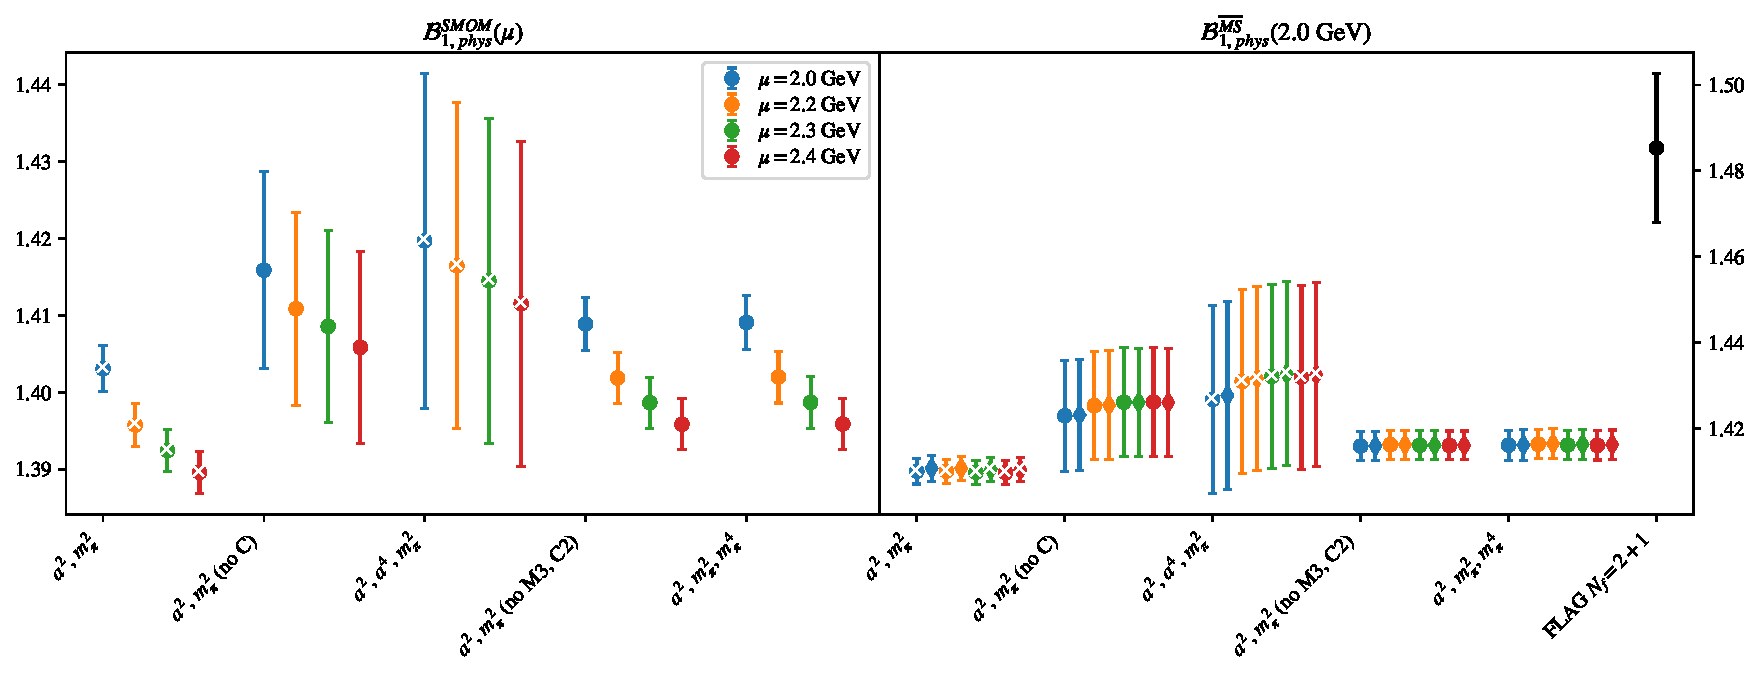
\includegraphics[page=1, width=1.1\textwidth]{VVpAA/SUSY/fit_summary.pdf}
\caption{$B_{1}$\\(left) $B_{phys}$ in RI/SMOM scheme from fit variations (fits with $p$-value $<0.05$ marked with ``$\times$"). \\(right) $B_{phys}$ in $\overline{MS}$ computed using $B^{\overline{MS}} = R^{\overline{MS}\leftarrow SMOM}(2.0)\sigma_{npt}(2.0,\mu) B^{SMOM}(\mu)$.}
\end{figure}
\clearpage
\begin{figure}
\centering
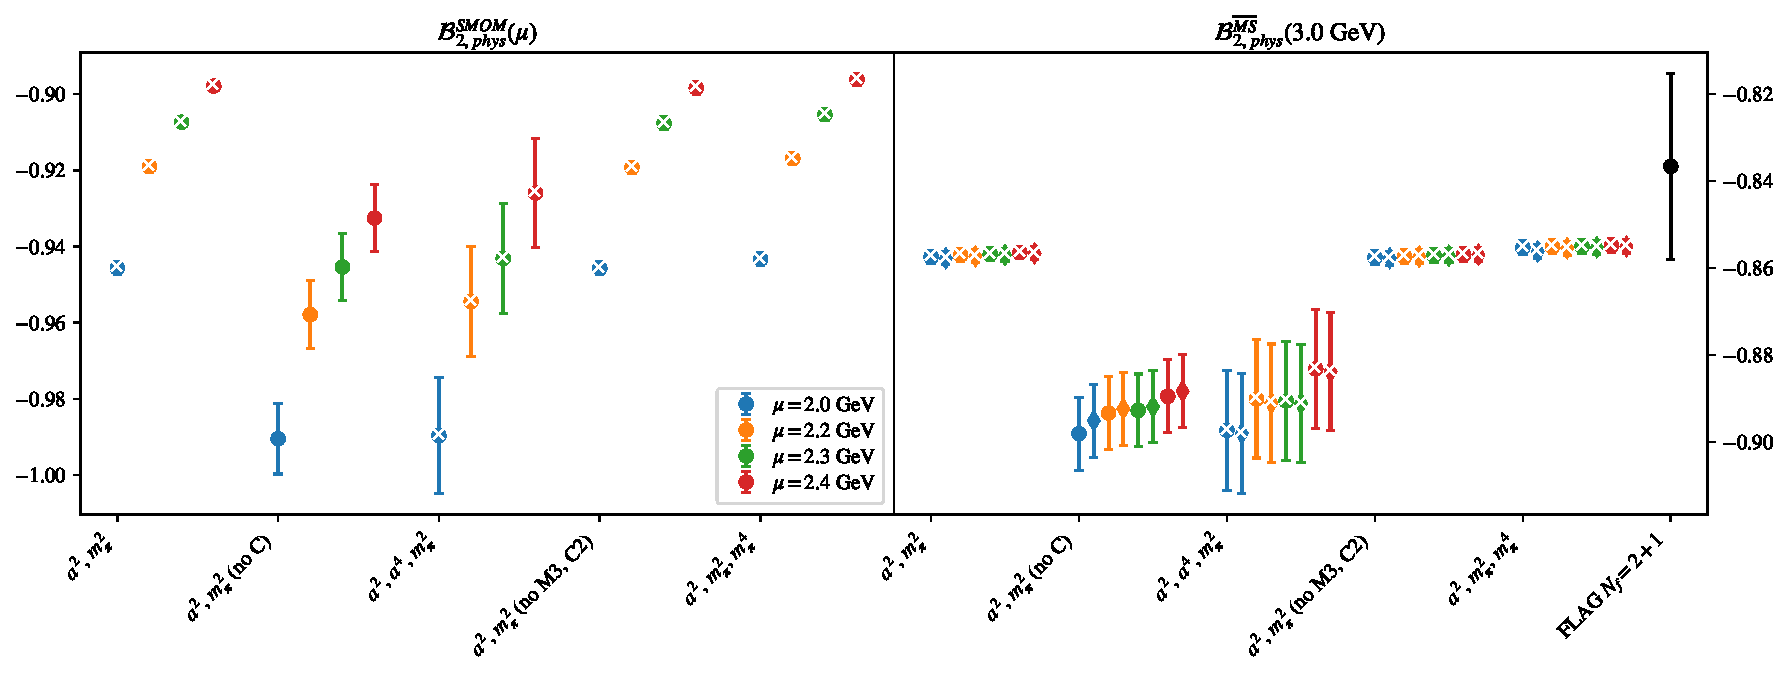
\includegraphics[page=1, width=1.1\textwidth]{VVmAA/SUSY/fit_summary.pdf}
\caption{$B_{2}$\\(left) $B_{phys}$ in RI/SMOM scheme from fit variations (fits with $p$-value $<0.05$ marked with ``$\times$"). \\(right) $B_{phys}$ in $\overline{MS}$ computed using $B^{\overline{MS}} = R^{\overline{MS}\leftarrow SMOM}(3.0)\sigma_{npt}(3.0,\mu) B^{SMOM}(\mu)$.}
\end{figure}
\clearpage
\begin{figure}
\centering
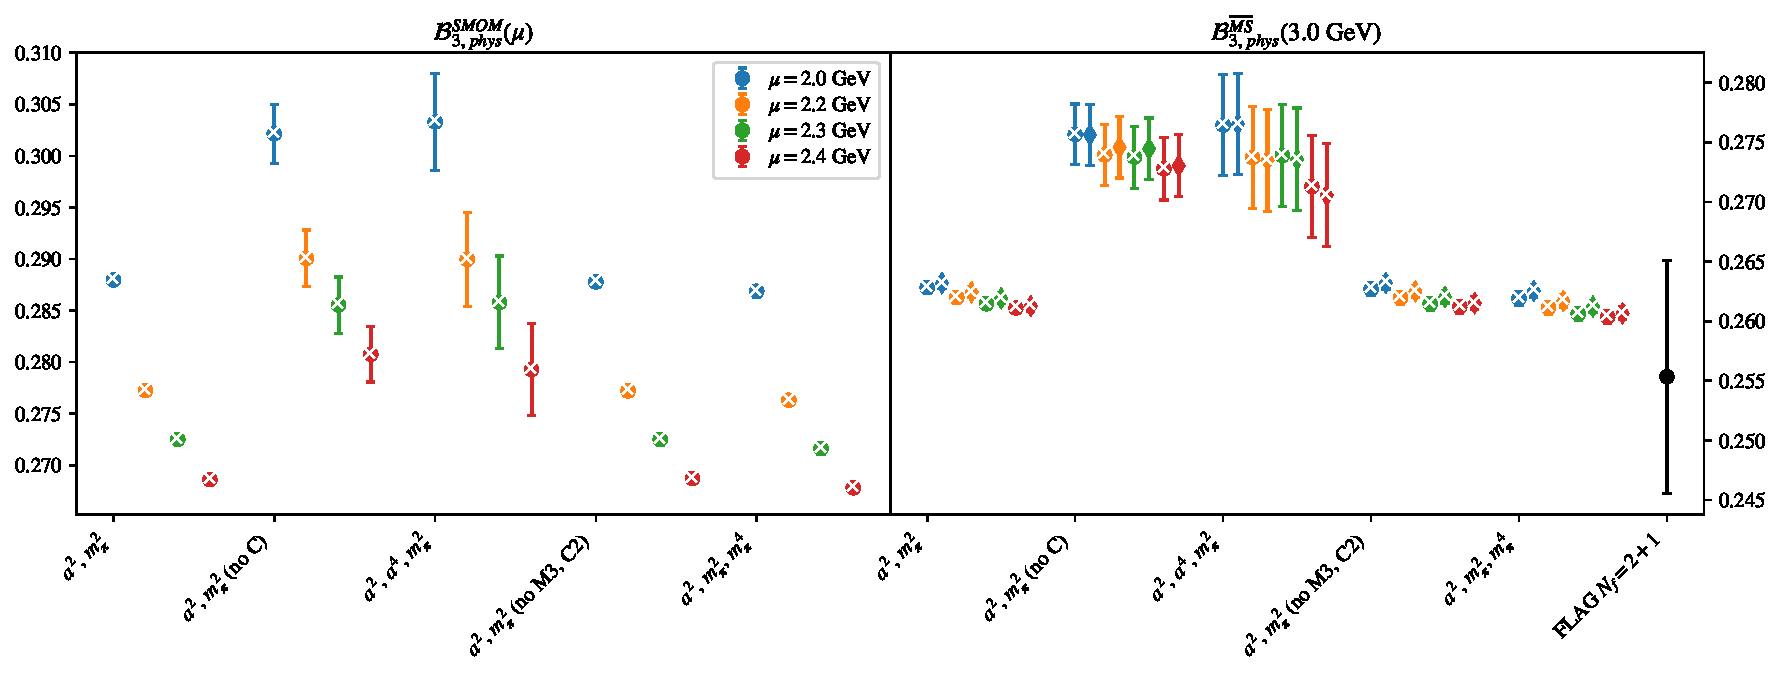
\includegraphics[page=1, width=1.1\textwidth]{SSmPP/SUSY/fit_summary.pdf}
\caption{$B_{3}$\\(left) $B_{phys}$ in RI/SMOM scheme from fit variations (fits with $p$-value $<0.05$ marked with ``$\times$"). \\(right) $B_{phys}$ in $\overline{MS}$ computed using $B^{\overline{MS}} = R^{\overline{MS}\leftarrow SMOM}(3.0)\sigma_{npt}(3.0,\mu) B^{SMOM}(\mu)$.}
\end{figure}
\clearpage
\begin{figure}
\centering
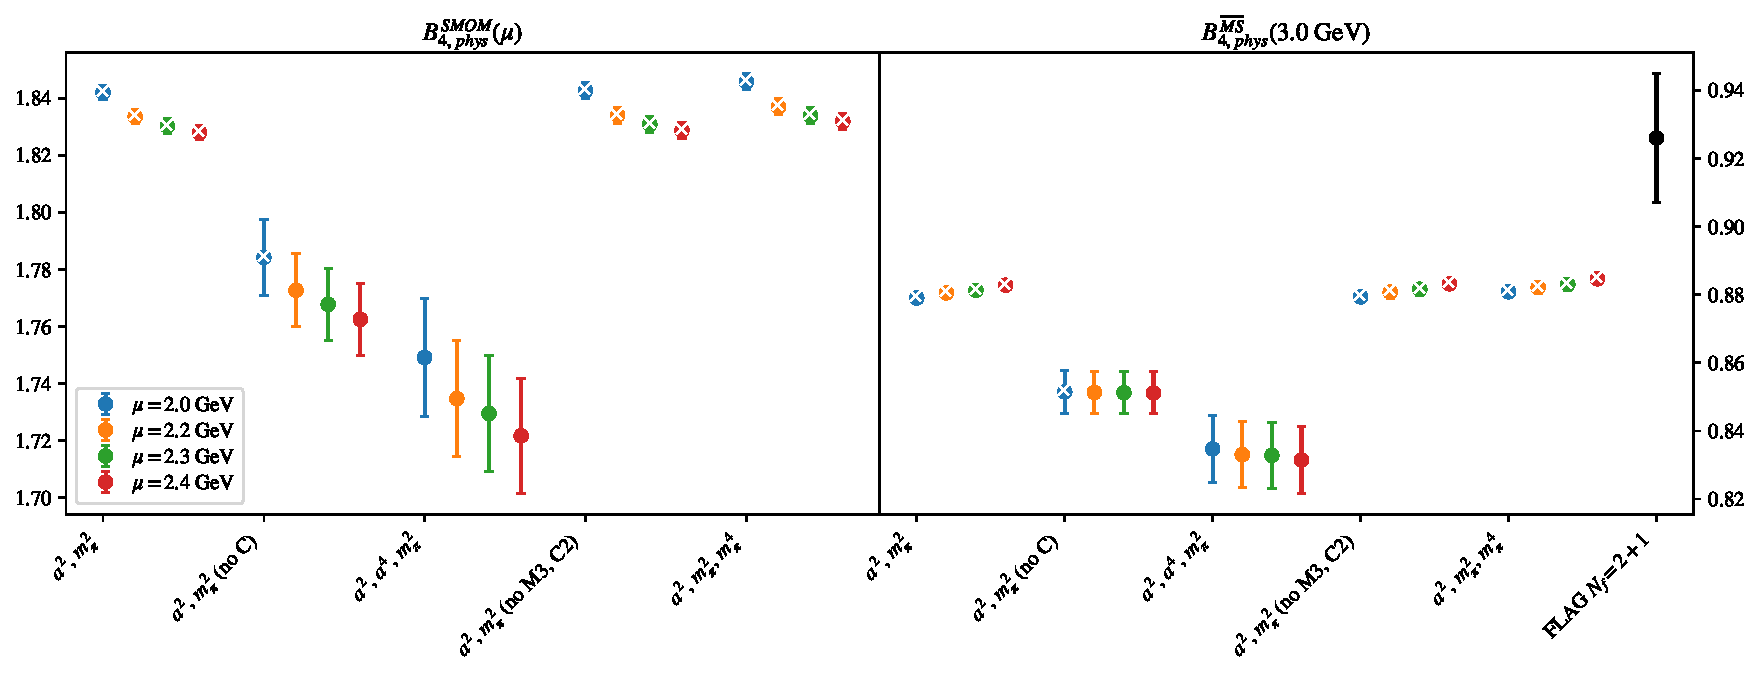
\includegraphics[page=1, width=1.1\textwidth]{SSpPP/SUSY/fit_summary.pdf}
\caption{$B_{4}$\\(left) $B_{phys}$ in RI/SMOM scheme from fit variations (fits with $p$-value $<0.05$ marked with ``$\times$"). \\(right) $B_{phys}$ in $\overline{MS}$ computed using $B^{\overline{MS}} = R^{\overline{MS}\leftarrow SMOM}(3.0)\sigma_{npt}(3.0,\mu) B^{SMOM}(\mu)$.}
\end{figure}
\clearpage
\begin{figure}
\centering
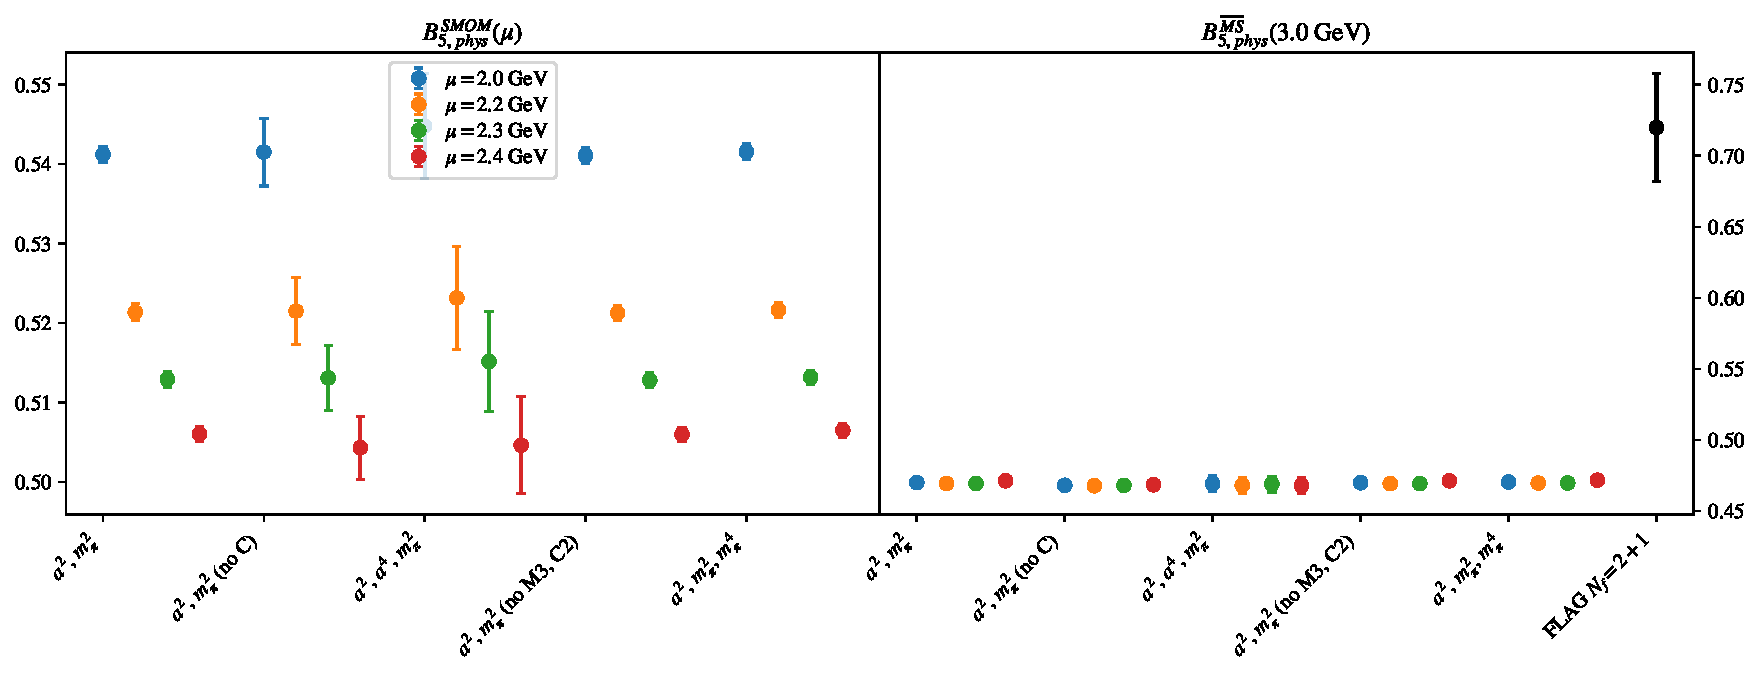
\includegraphics[page=1, width=1.1\textwidth]{TT/SUSY/fit_summary.pdf}
\caption{$B_{5}$\\(left) $B_{phys}$ in RI/SMOM scheme from fit variations (fits with $p$-value $<0.05$ marked with ``$\times$"). \\(right) $B_{phys}$ in $\overline{MS}$ computed using $B^{\overline{MS}} = R^{\overline{MS}\leftarrow SMOM}(3.0)\sigma_{npt}(3.0,\mu) B^{SMOM}(\mu)$.}
\end{figure}
\clearpage
\section{$B_1$}
\begin{table}[h!]
\begin{center}
\begin{tabular}{|c|c|c|c|c|c|}
\hline
$\mu$ (GeV) & $a^2$, $m_\pi^2$& $a^2$, $m_\pi^2$ (no C)& $a^2$, $a^4$, $m_\pi^2$& $a^2$, $m_\pi^2$ (no M3, C2)& $a^2$, $m_\pi^2$, $m_\pi^4$\\
\hline
2.0& \hyperlink{VVpAA/SUSY/a2m2_20.pdf.1}{\textbf{0.5264(10)}: 1.858 (0.098)} & \hyperlink{VVpAA/SUSY/a2m2noC_20.pdf.1}{\textbf{0.5310(47)}: 0.876 (0.417)} & \hyperlink{VVpAA/SUSY/a2a4m2_20.pdf.1}{\textbf{0.5327(81)}: 2.173 (0.069)} & \hyperlink{VVpAA/SUSY/a2m2mcut_20.pdf.1}{\textbf{0.5283(12)}: 0.248 (0.863)} & \hyperlink{VVpAA/SUSY/a2m2m4_20.pdf.1}{\textbf{0.5284(12)}: 0.661 (0.619)}\\
2.2& \hyperlink{VVpAA/SUSY/a2m2_22.pdf.1}{\textbf{0.5236(10)}: 2.214 (0.05)} & \hyperlink{VVpAA/SUSY/a2m2noC_22.pdf.1}{\textbf{0.5291(46)}: 1.143 (0.319)} & \hyperlink{VVpAA/SUSY/a2a4m2_22.pdf.1}{\textbf{0.5314(79)}: 2.525 (0.039)} & \hyperlink{VVpAA/SUSY/a2m2mcut_22.pdf.1}{\textbf{0.5257(12)}: 0.36 (0.782)} & \hyperlink{VVpAA/SUSY/a2m2m4_22.pdf.1}{\textbf{0.5257(12)}: 0.923 (0.449)}\\
2.3& \hyperlink{VVpAA/SUSY/a2m2_23.pdf.1}{\textbf{0.5224(10)}: 2.304 (0.042)} & \hyperlink{VVpAA/SUSY/a2m2noC_23.pdf.1}{\textbf{0.5282(46)}: 1.197 (0.302)} & \hyperlink{VVpAA/SUSY/a2a4m2_23.pdf.1}{\textbf{0.5306(78)}: 2.605 (0.034)} & \hyperlink{VVpAA/SUSY/a2m2mcut_23.pdf.1}{\textbf{0.5245(12)}: 0.411 (0.745)} & \hyperlink{VVpAA/SUSY/a2m2m4_23.pdf.1}{\textbf{0.5245(12)}: 0.993 (0.41)}\\
2.4& \hyperlink{VVpAA/SUSY/a2m2_24.pdf.1}{\textbf{0.5213(10)}: 2.348 (0.039)} & \hyperlink{VVpAA/SUSY/a2m2noC_24.pdf.1}{\textbf{0.5271(46)}: 1.223 (0.294)} & \hyperlink{VVpAA/SUSY/a2a4m2_24.pdf.1}{\textbf{0.5295(78)}: 2.663 (0.031)} & \hyperlink{VVpAA/SUSY/a2m2mcut_24.pdf.1}{\textbf{0.5234(12)}: 0.411 (0.745)} & \hyperlink{VVpAA/SUSY/a2m2m4_24.pdf.1}{\textbf{0.5235(12)}: 1.005 (0.403)}\\
\hline
\end{tabular}
\caption{Physical point value from chiral and continuum extrapolation at renormalisation scale $\mu$. Entries are \textbf{value(error)}: $\chi^2/\text{DOF}$ ($p$-value).}
\end{center}
\end{table}
\begin{table}[h!]
\begin{center}
\begin{tabular}{|c c|c|c|c|c|c|}
\hline
$\mu$ (GeV) &  & $a^2$, $m_\pi^2$& $a^2$, $m_\pi^2$ (no C)& $a^2$, $a^4$, $m_\pi^2$& $a^2$, $m_\pi^2$ (no M3, C2)& $a^2$, $m_\pi^2$, $m_\pi^4$\\
\hline
\multirow{2}{0.5in}{2.0} & $\alpha$ & 0.0937(71)& 0.047(53)& -0.017& 0.0815(83)& 0.0813(82)\\
 & $\beta$ & 0.00261(14)& 0.00223(27)& 0.00263(15)& 0.00189(28)& 0.00031(90)\\
\hline
\multirow{2}{0.5in}{2.2} & $\alpha$ & 0.0977(70)& 0.041(52)& -0.038& 0.0847(83)& 0.0846(82)\\
 & $\beta$ & 0.00261(14)& 0.00220(27)& 0.00264(14)& 0.00184(28)& 0.00020(89)\\
\hline
\multirow{2}{0.5in}{2.3} & $\alpha$ & 0.0992(70)& 0.039(52)& -0.045& 0.0859(83)& 0.0859(82)\\
 & $\beta$ & 0.00262(14)& 0.00220(27)& 0.00265(14)& 0.00184(28)& 0.00018(89)\\
\hline
\multirow{2}{0.5in}{2.4} & $\alpha$ & 0.0999(70)& 0.040(52)& -0.044& 0.0864(83)& 0.0864(82)\\
 & $\beta$ & 0.00263(14)& 0.00220(27)& 0.00266(14)& 0.00184(28)& 0.00017(89)\\
\hline
\end{tabular}
\caption{Fit values of coefficients in $B = B_{phys} + \mathbf{\alpha} a^2 + \mathbf{\beta}\left(\frac{m_\pi^2}{f_\pi^2}-\frac{m_{\pi,PDG}^2}{f_\pi^2}\right) + \ldots$.}
\end{center}
\end{table}
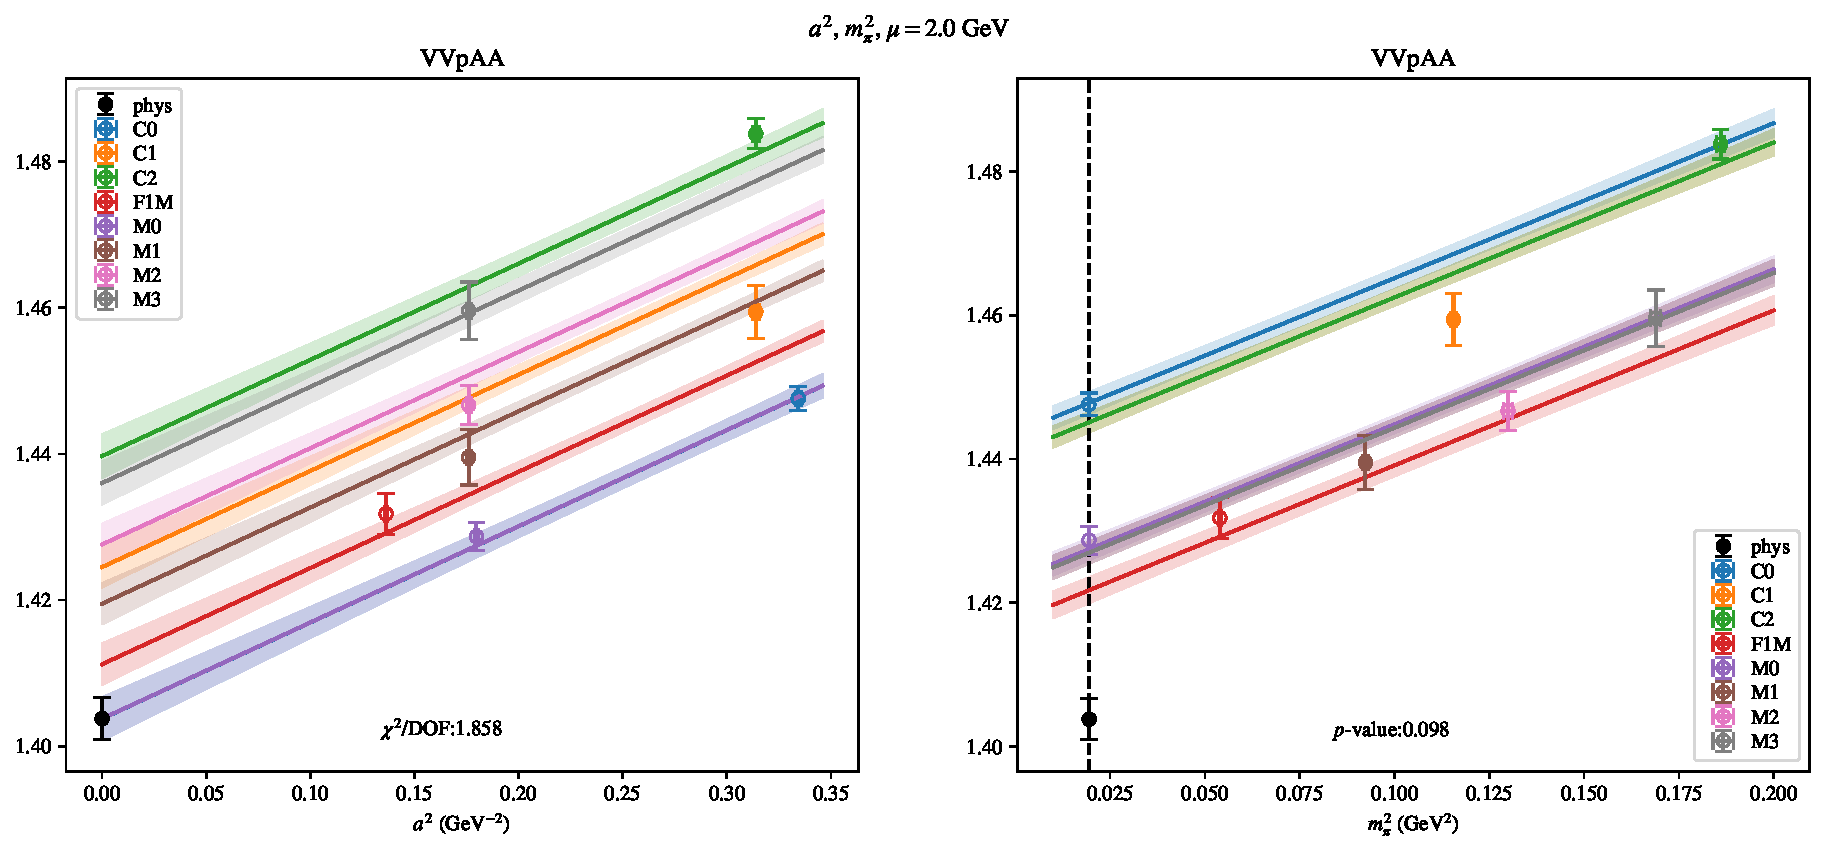
\includepdf[link, pages=-]{VVpAA/SUSY/a2m2_20.pdf}
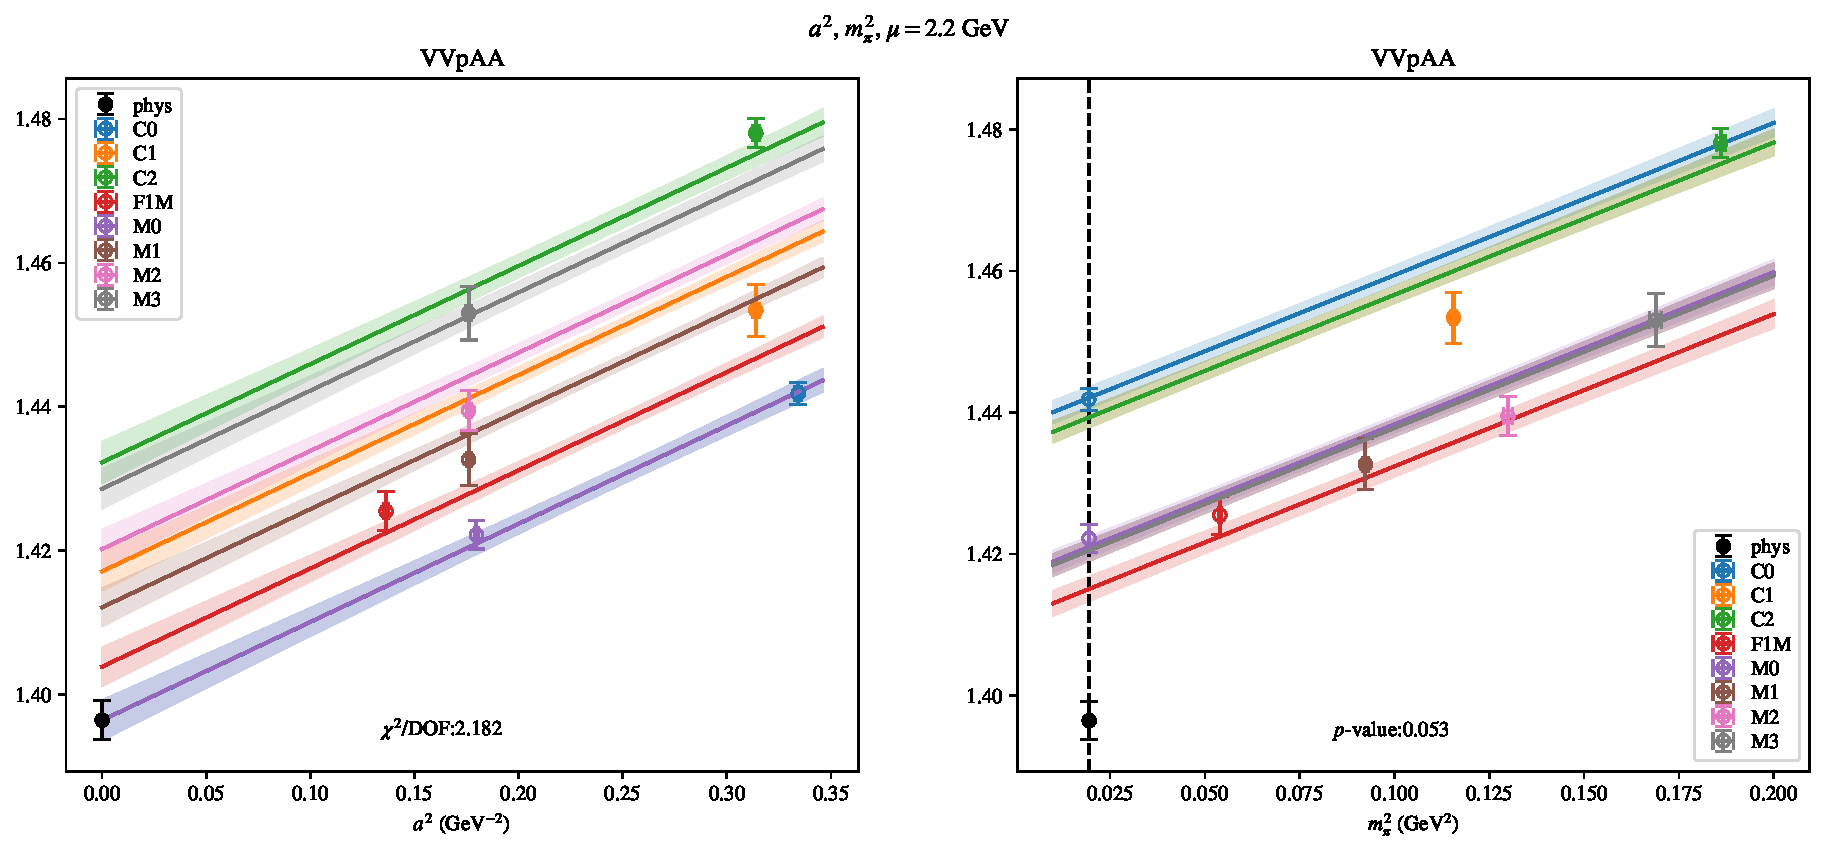
\includepdf[link, pages=-]{VVpAA/SUSY/a2m2_22.pdf}
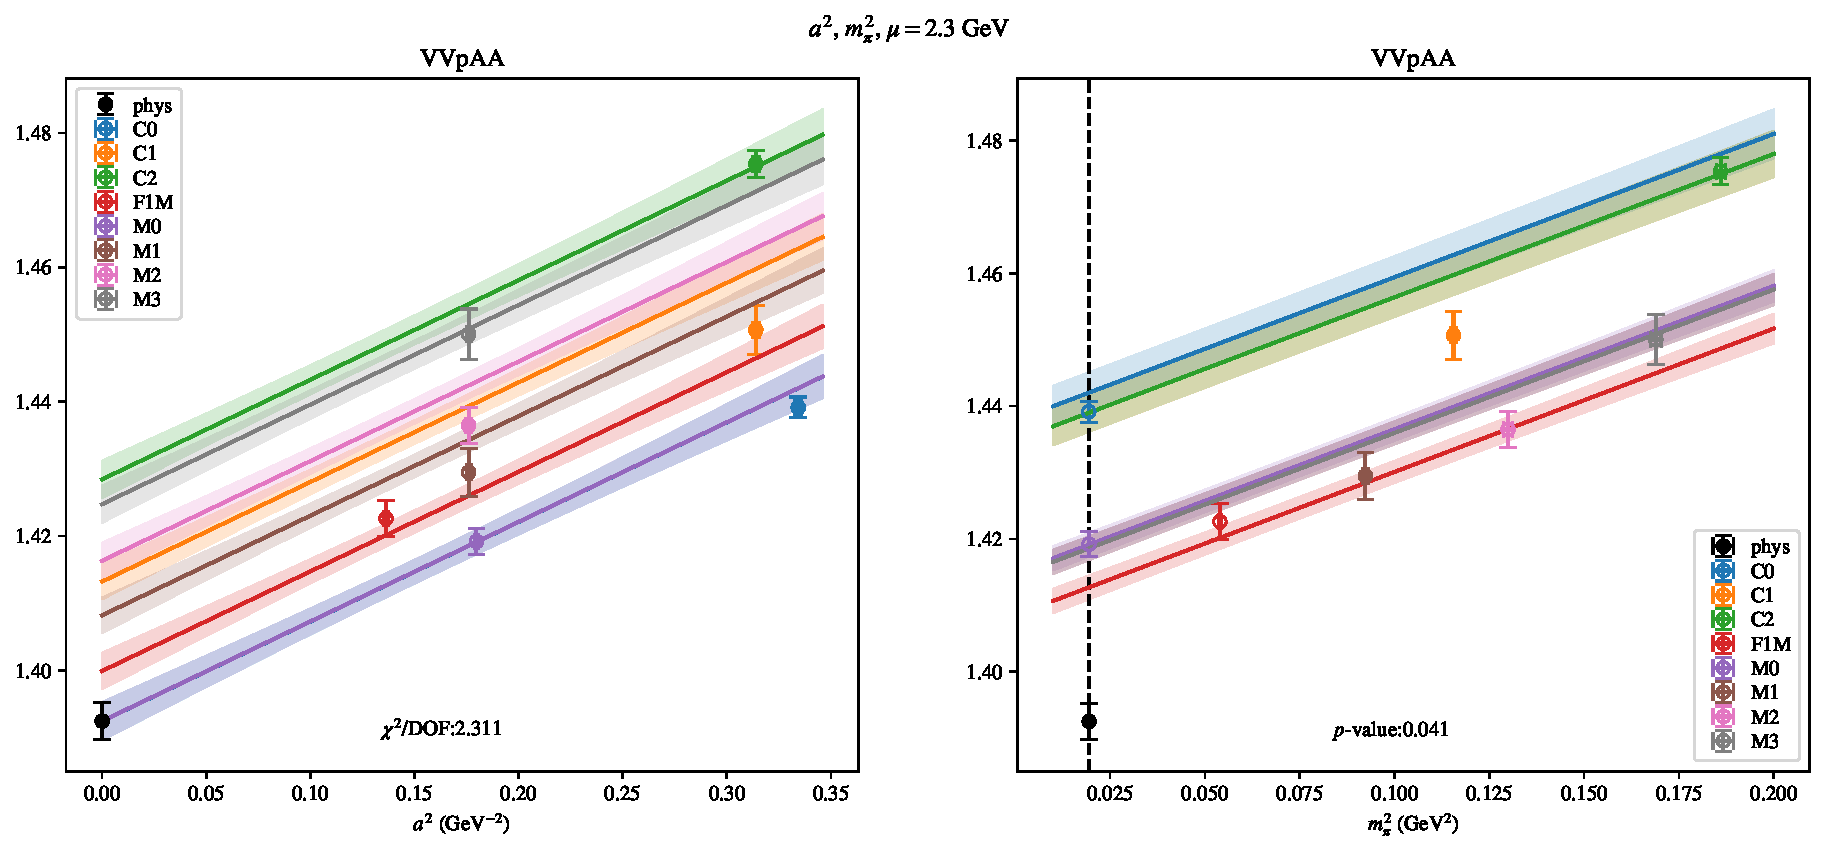
\includepdf[link, pages=-]{VVpAA/SUSY/a2m2_23.pdf}
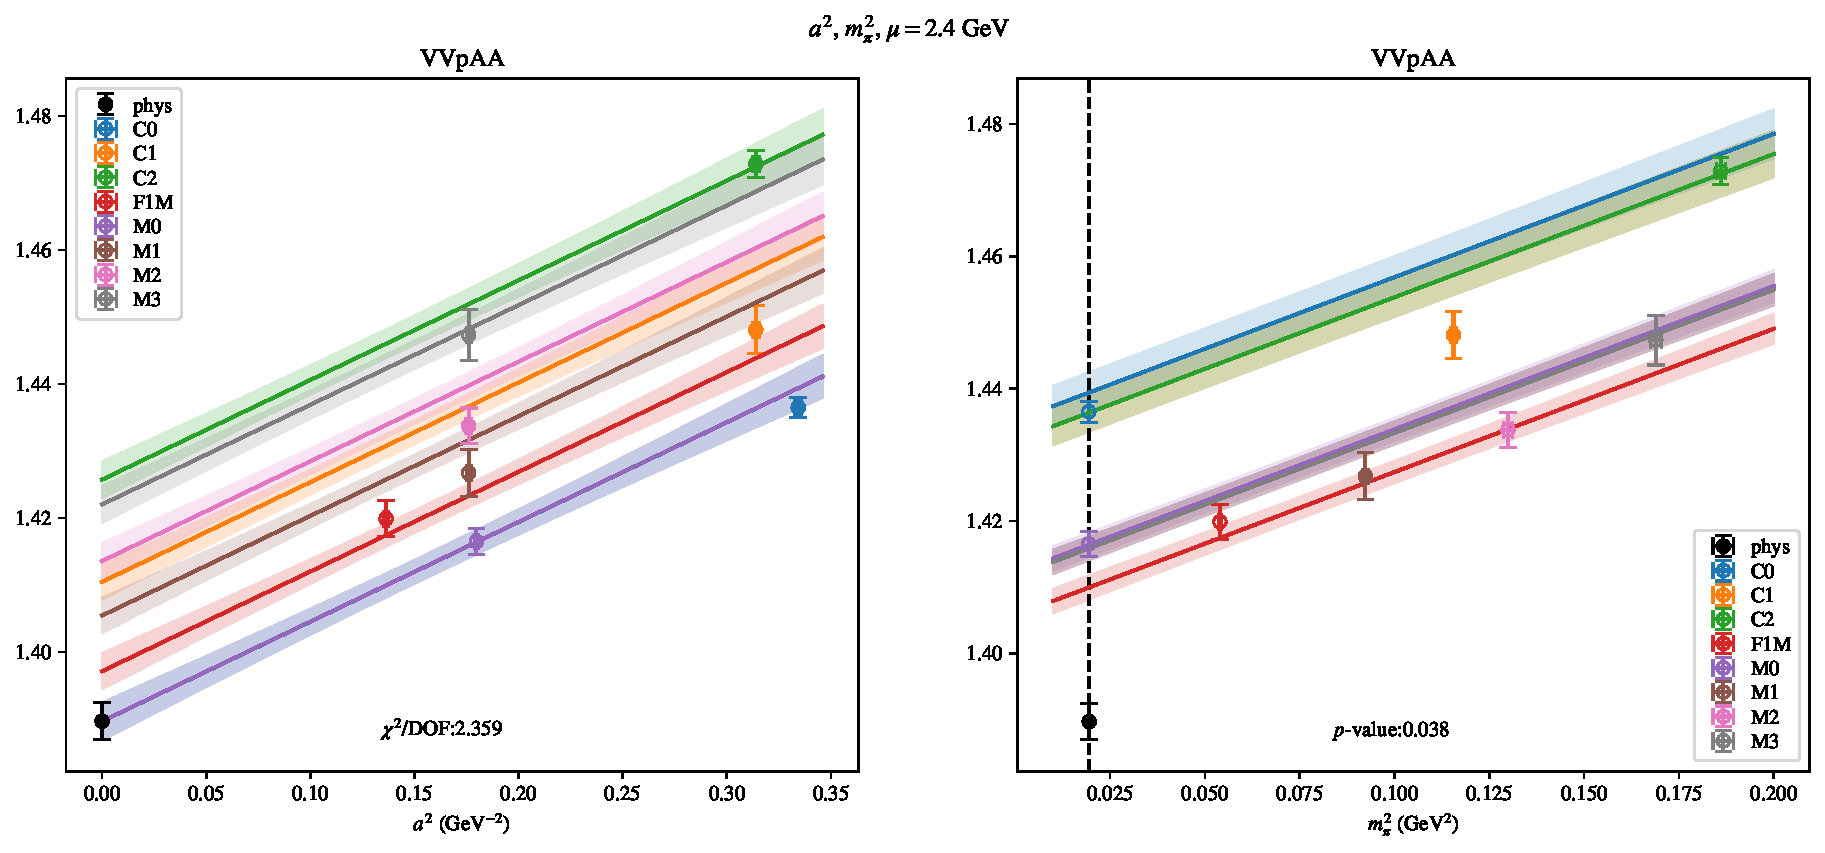
\includepdf[link, pages=-]{VVpAA/SUSY/a2m2_24.pdf}
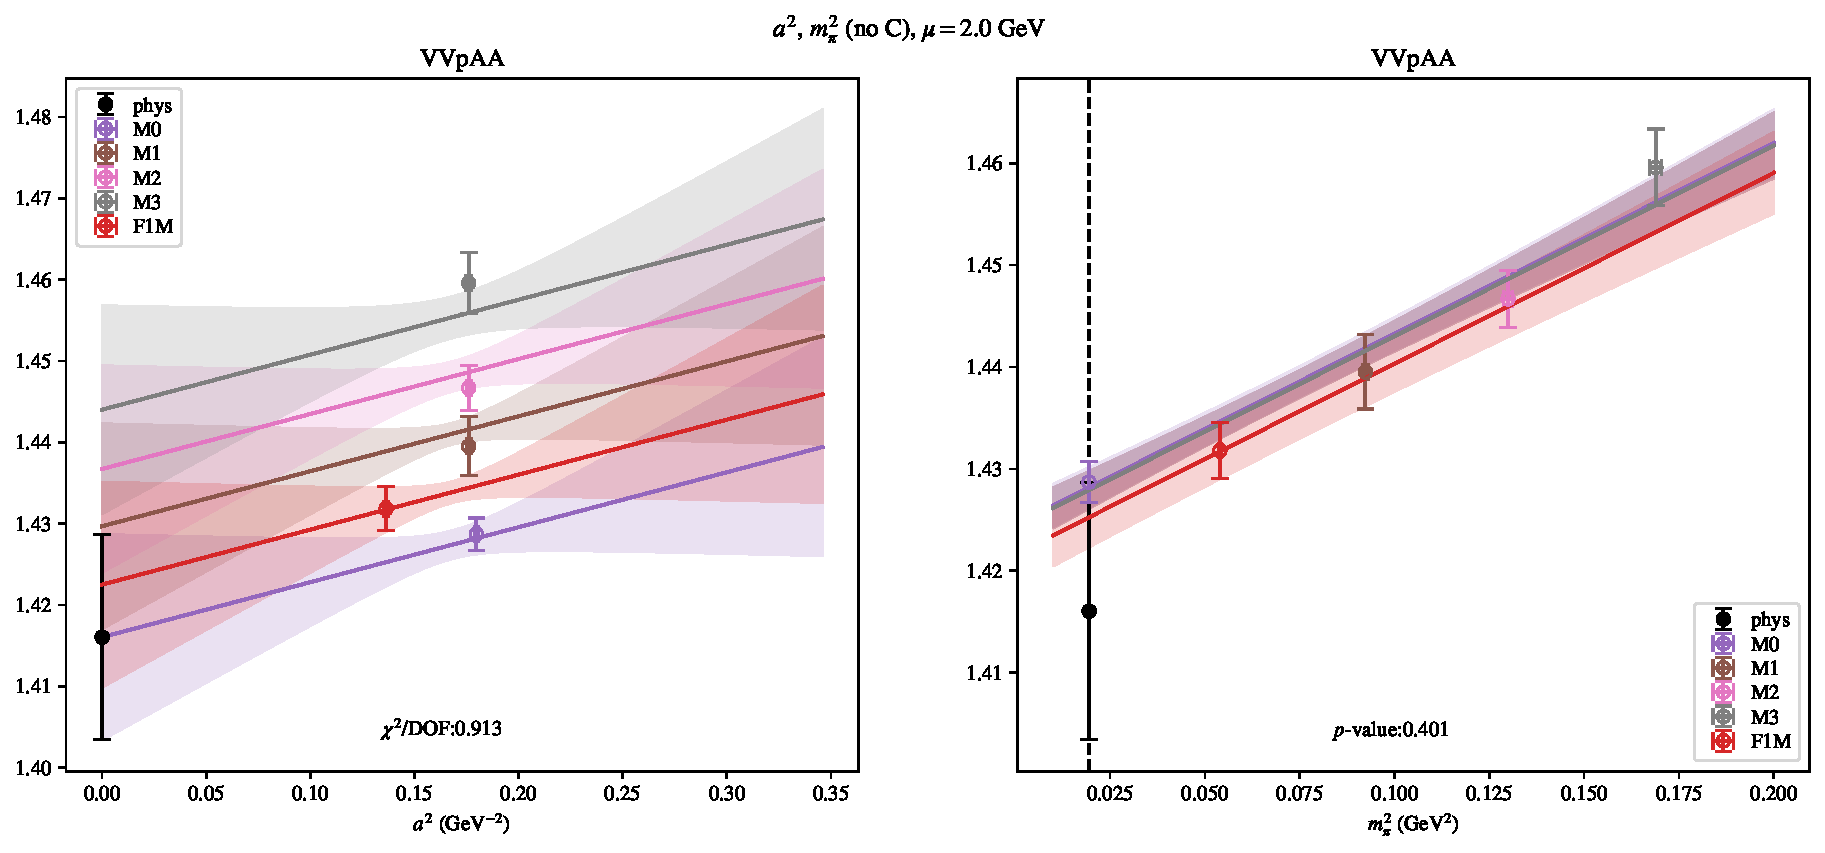
\includepdf[link, pages=-]{VVpAA/SUSY/a2m2noC_20.pdf}
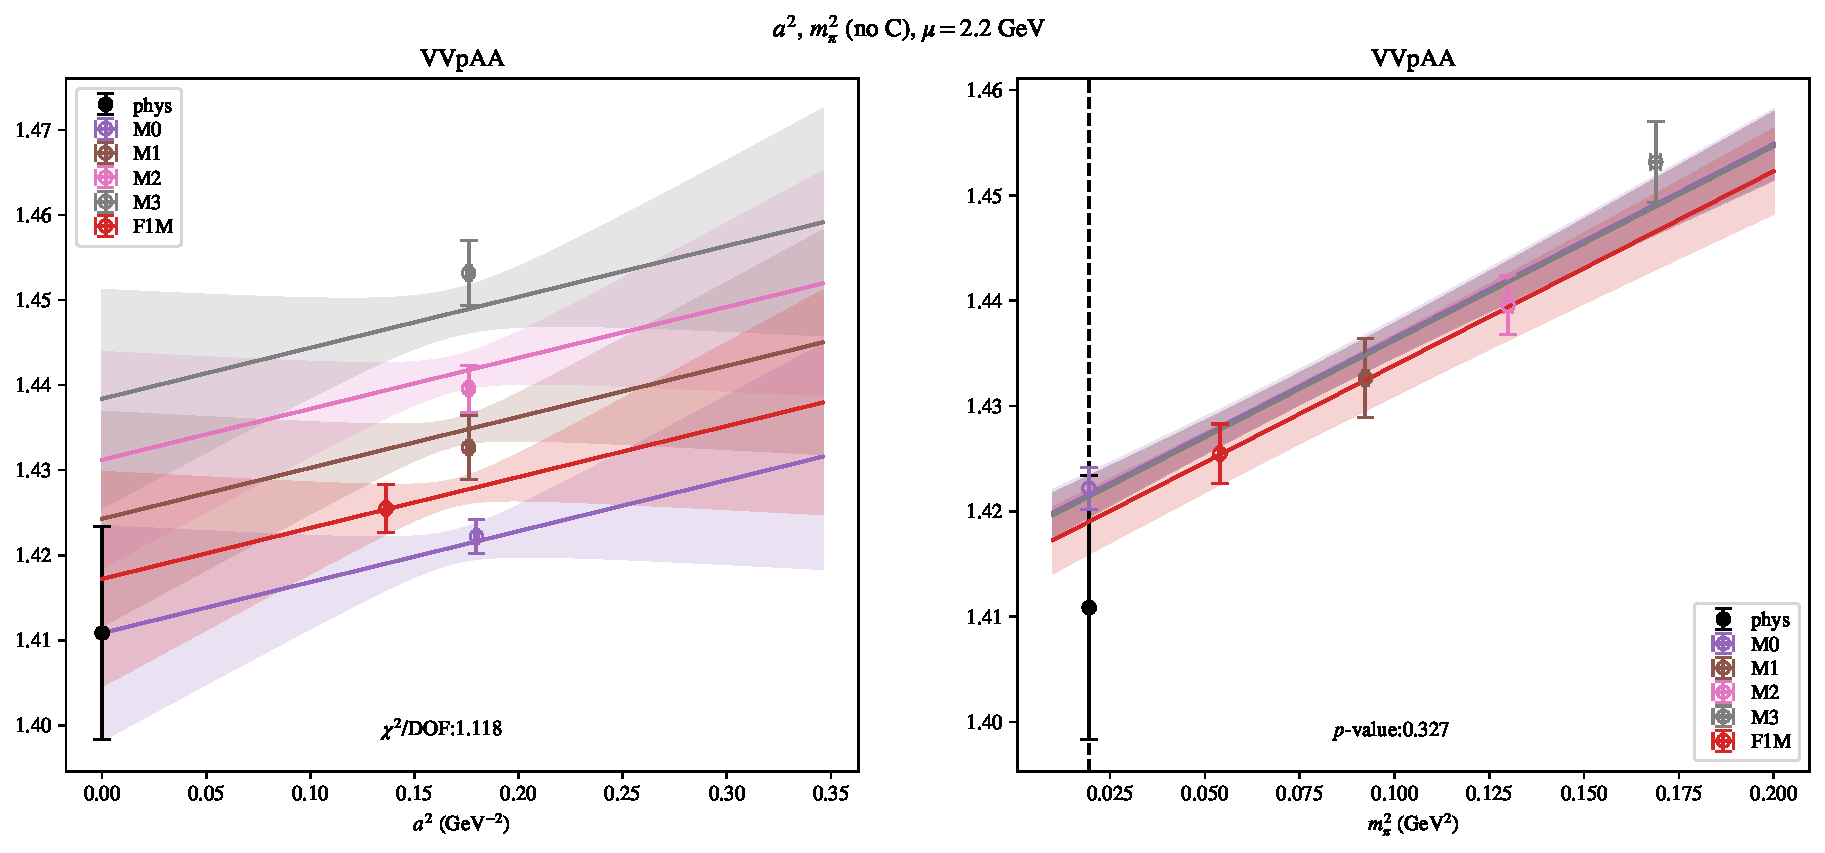
\includepdf[link, pages=-]{VVpAA/SUSY/a2m2noC_22.pdf}
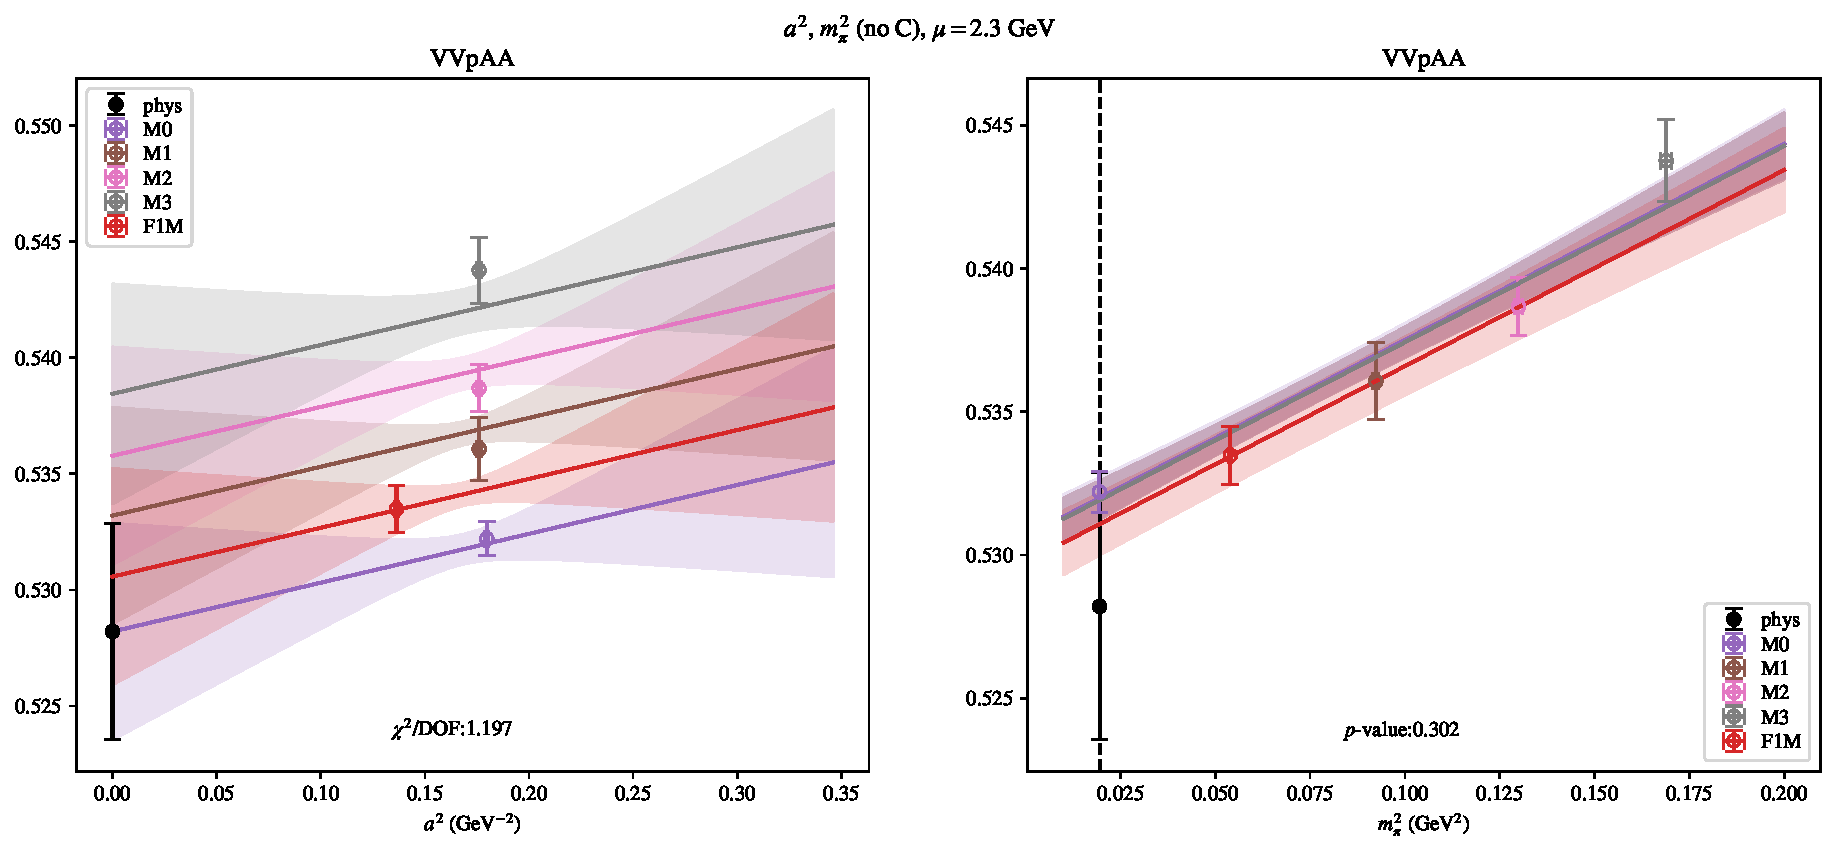
\includepdf[link, pages=-]{VVpAA/SUSY/a2m2noC_23.pdf}
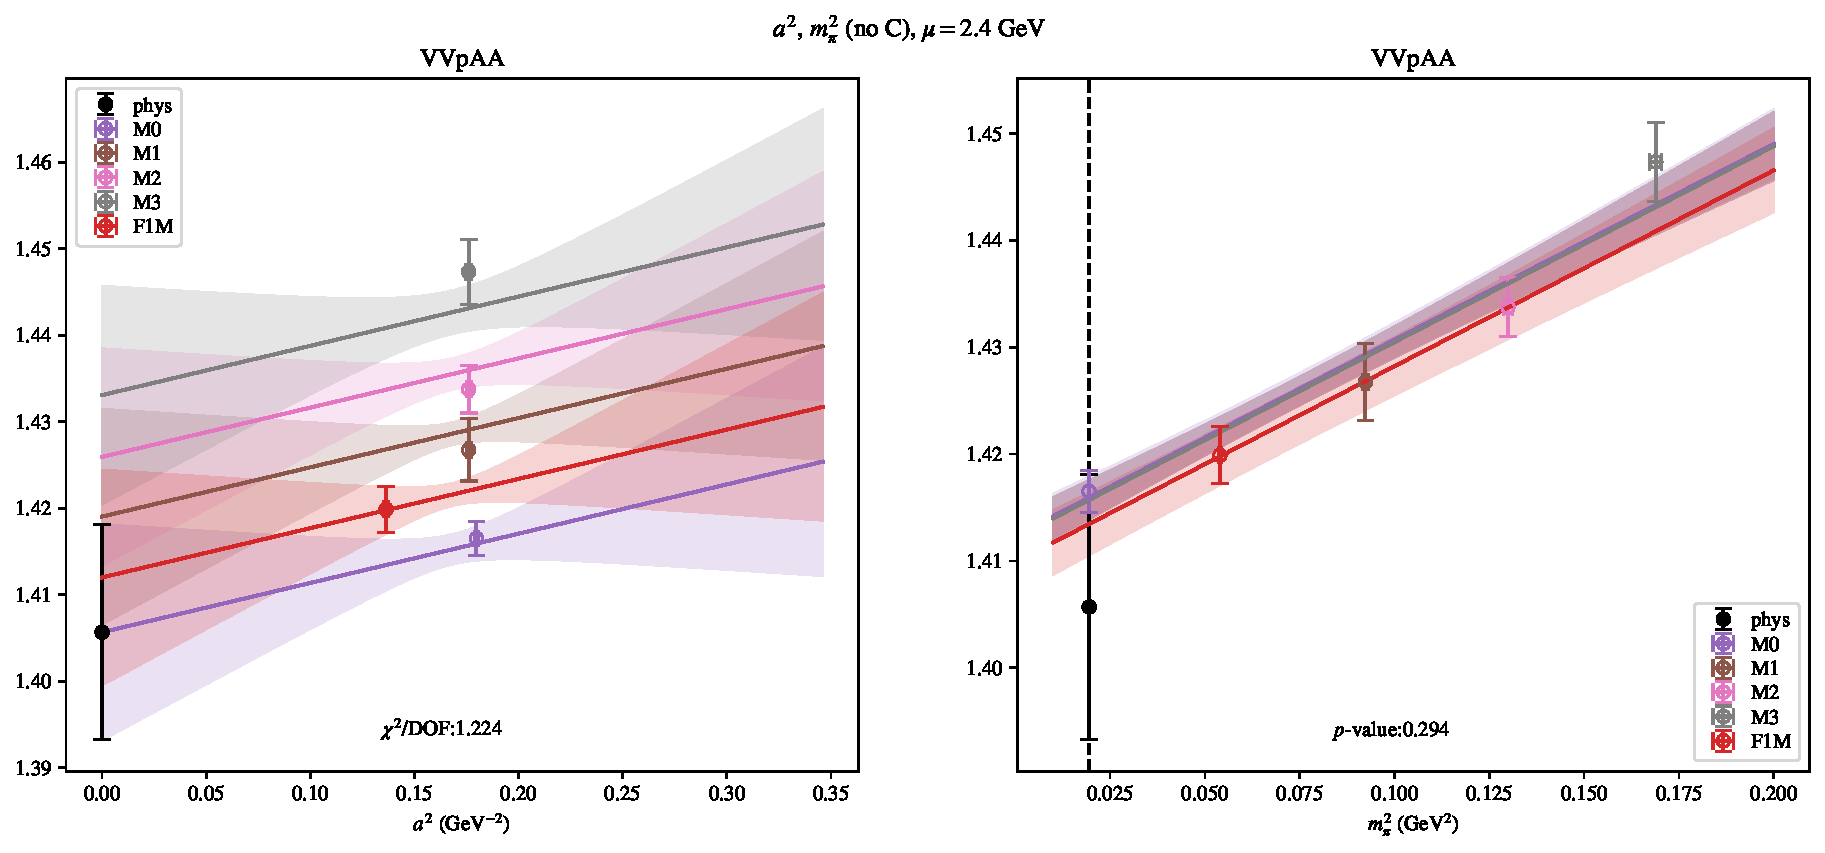
\includepdf[link, pages=-]{VVpAA/SUSY/a2m2noC_24.pdf}
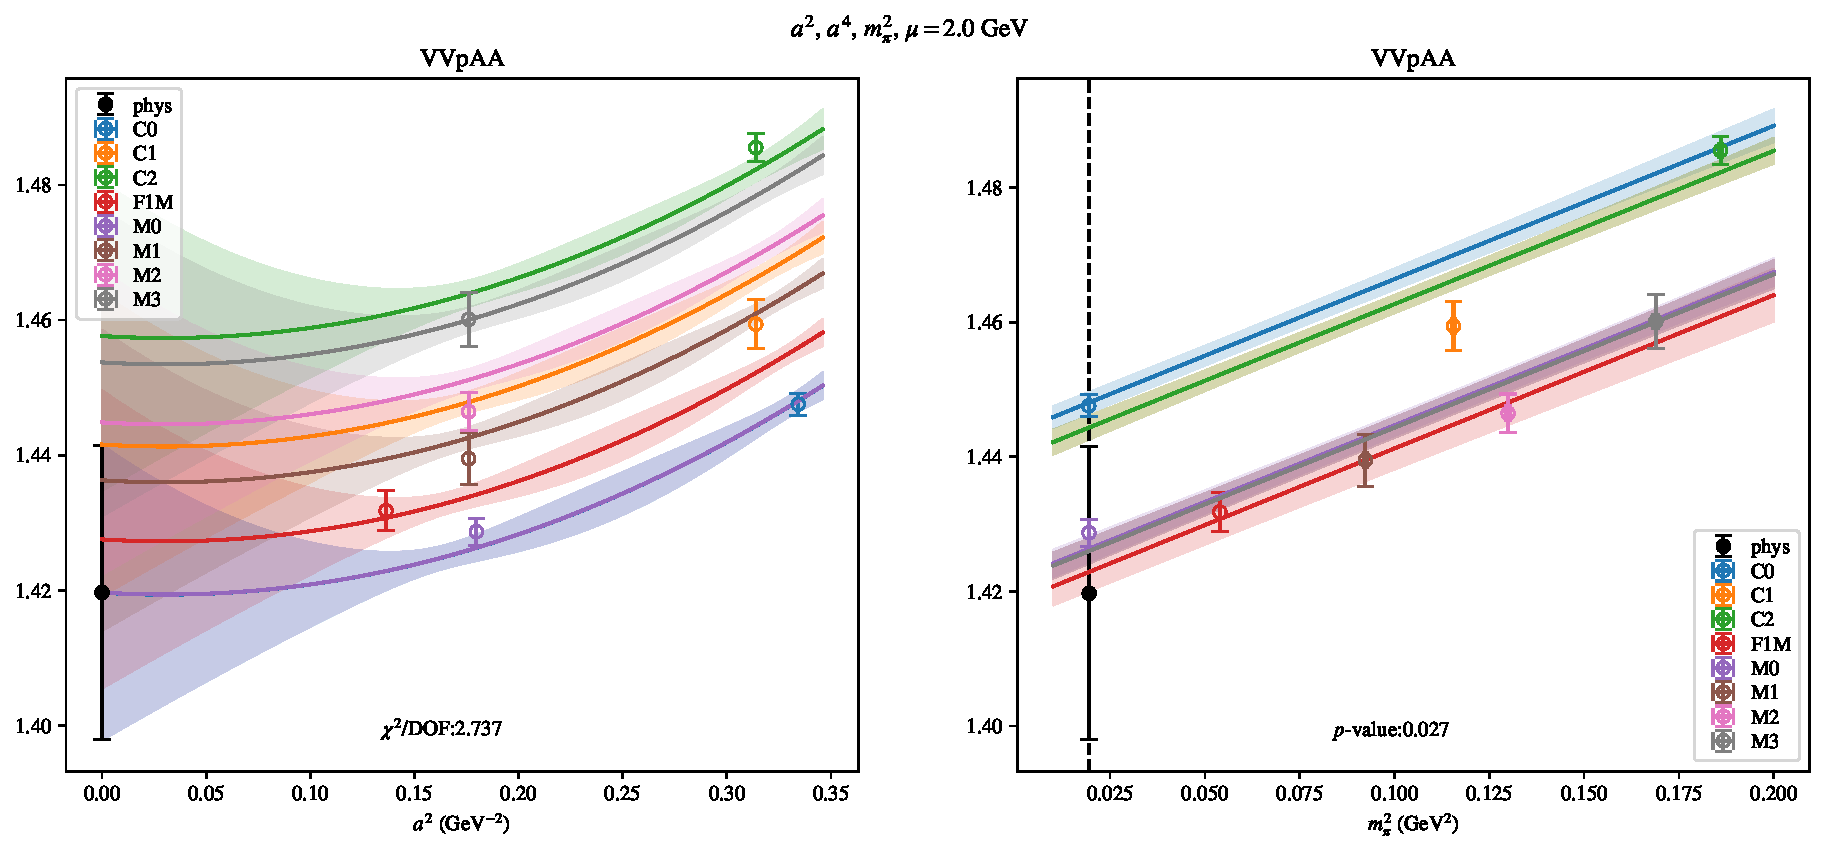
\includepdf[link, pages=-]{VVpAA/SUSY/a2a4m2_20.pdf}
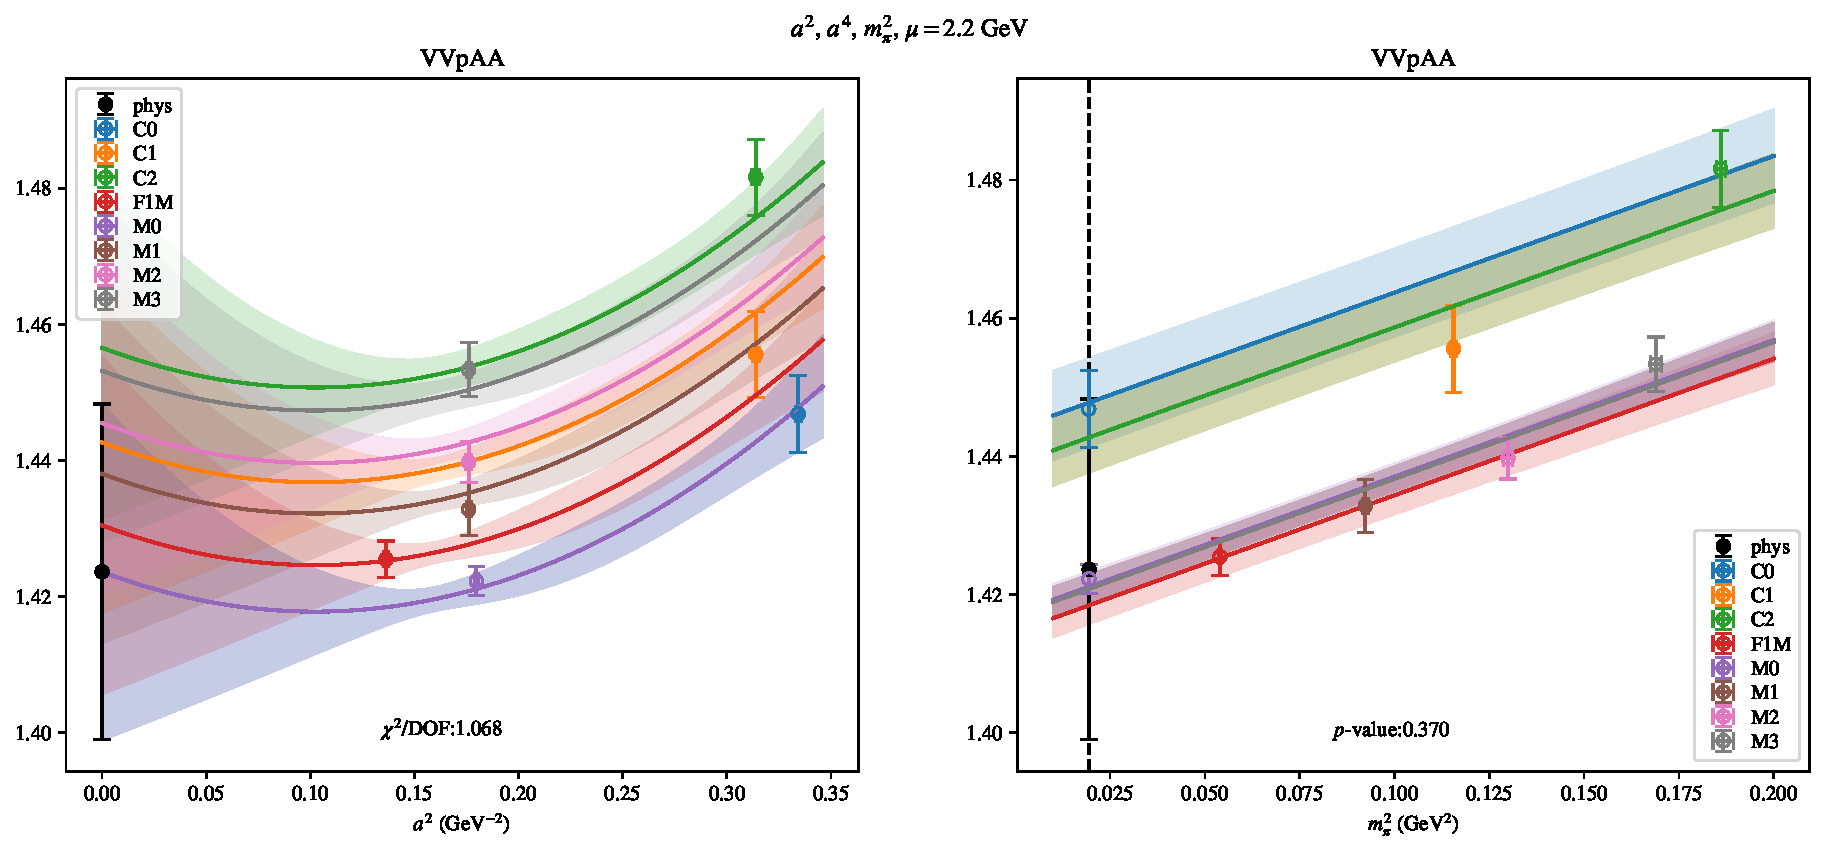
\includepdf[link, pages=-]{VVpAA/SUSY/a2a4m2_22.pdf}
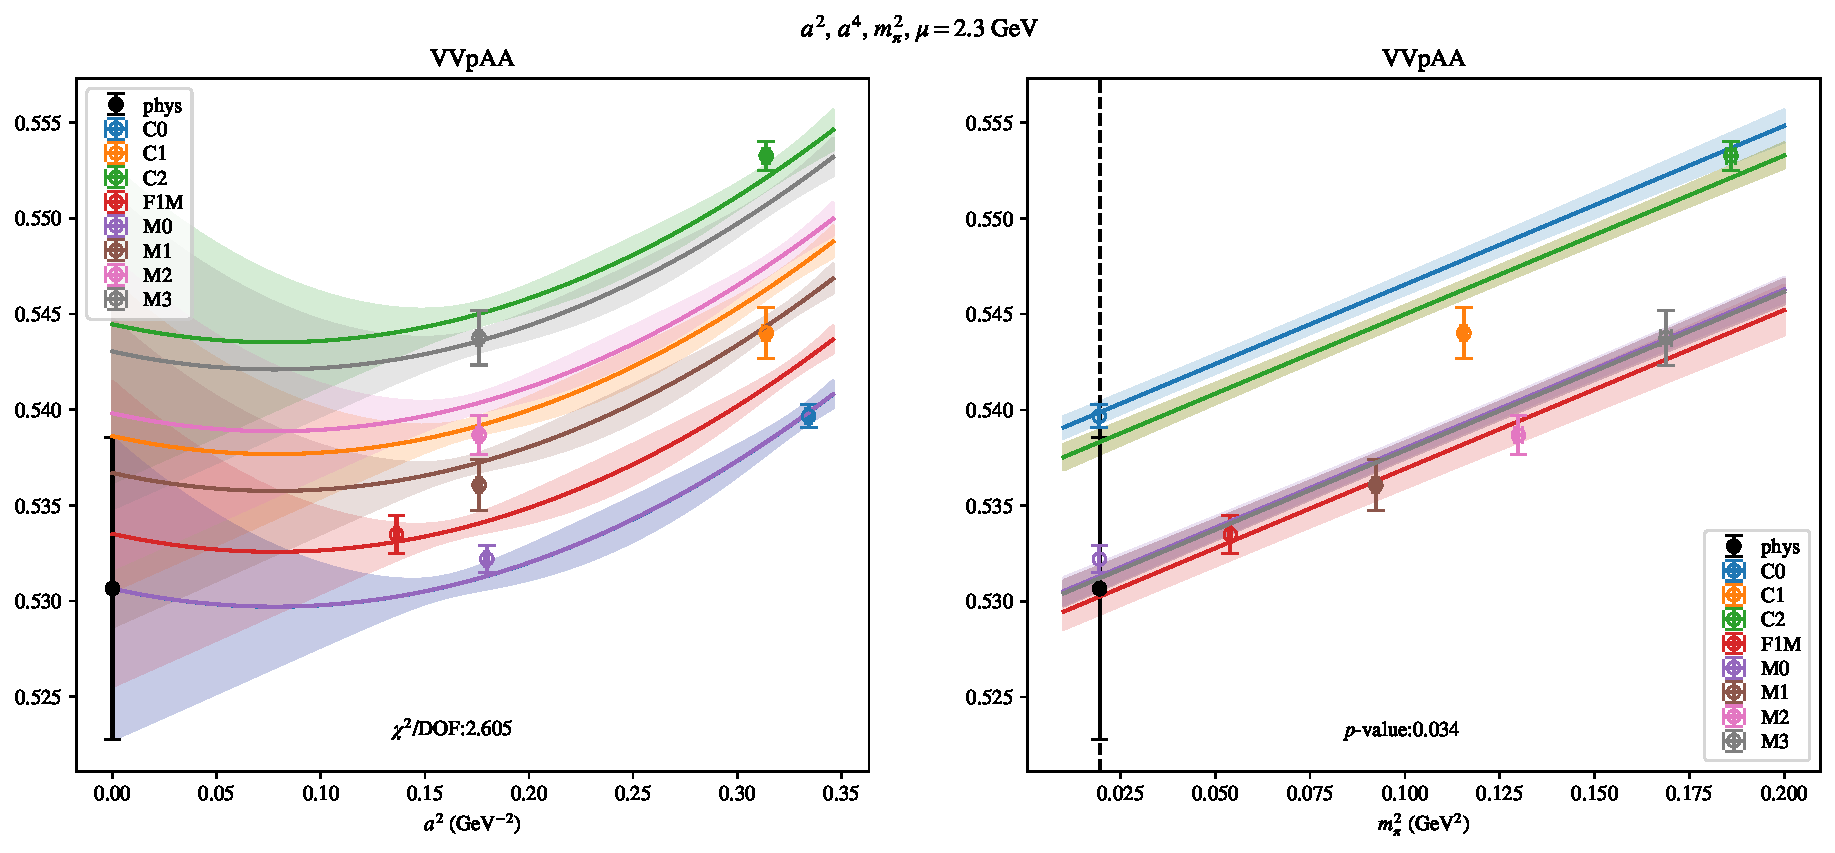
\includepdf[link, pages=-]{VVpAA/SUSY/a2a4m2_23.pdf}
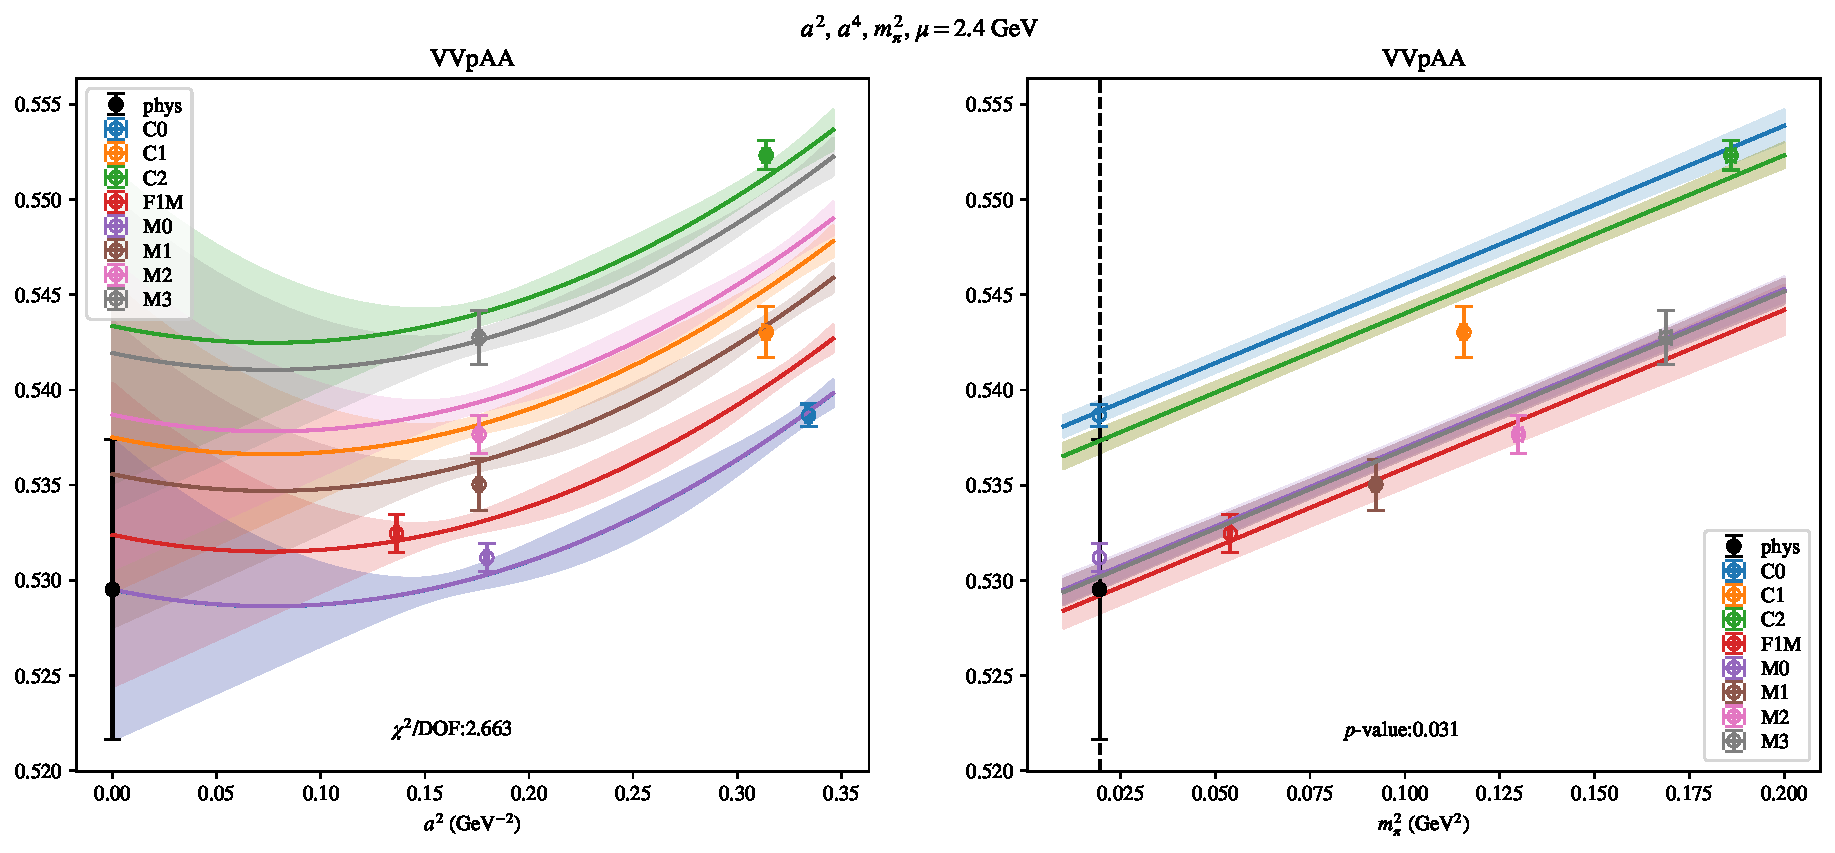
\includepdf[link, pages=-]{VVpAA/SUSY/a2a4m2_24.pdf}
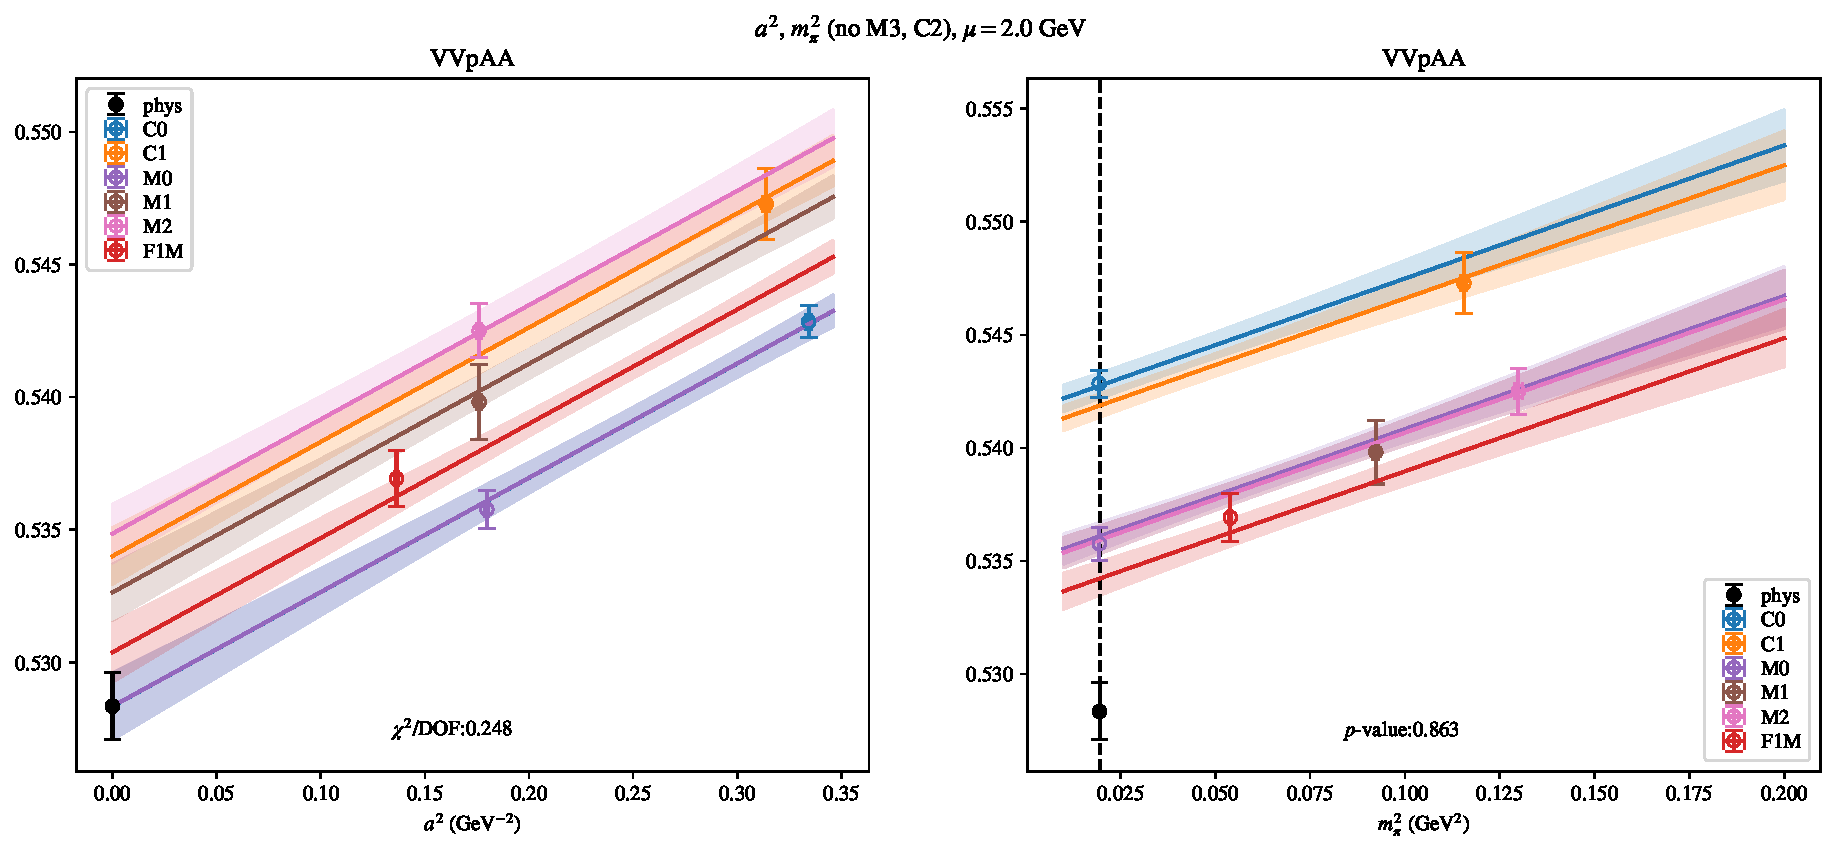
\includepdf[link, pages=-]{VVpAA/SUSY/a2m2mcut_20.pdf}
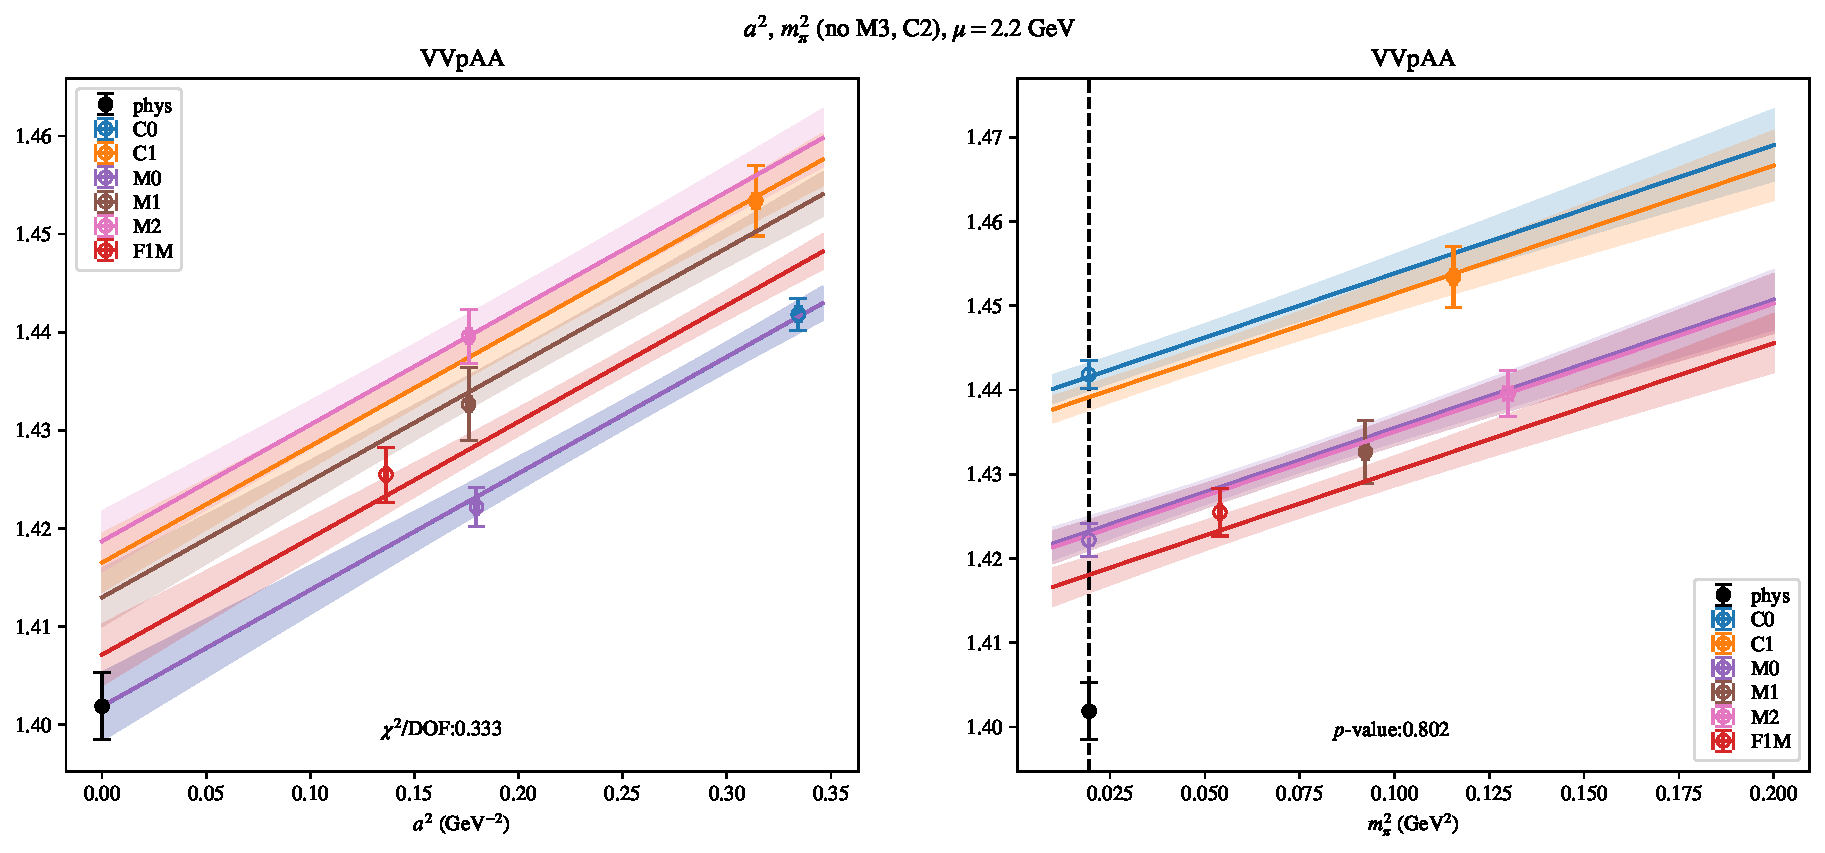
\includepdf[link, pages=-]{VVpAA/SUSY/a2m2mcut_22.pdf}
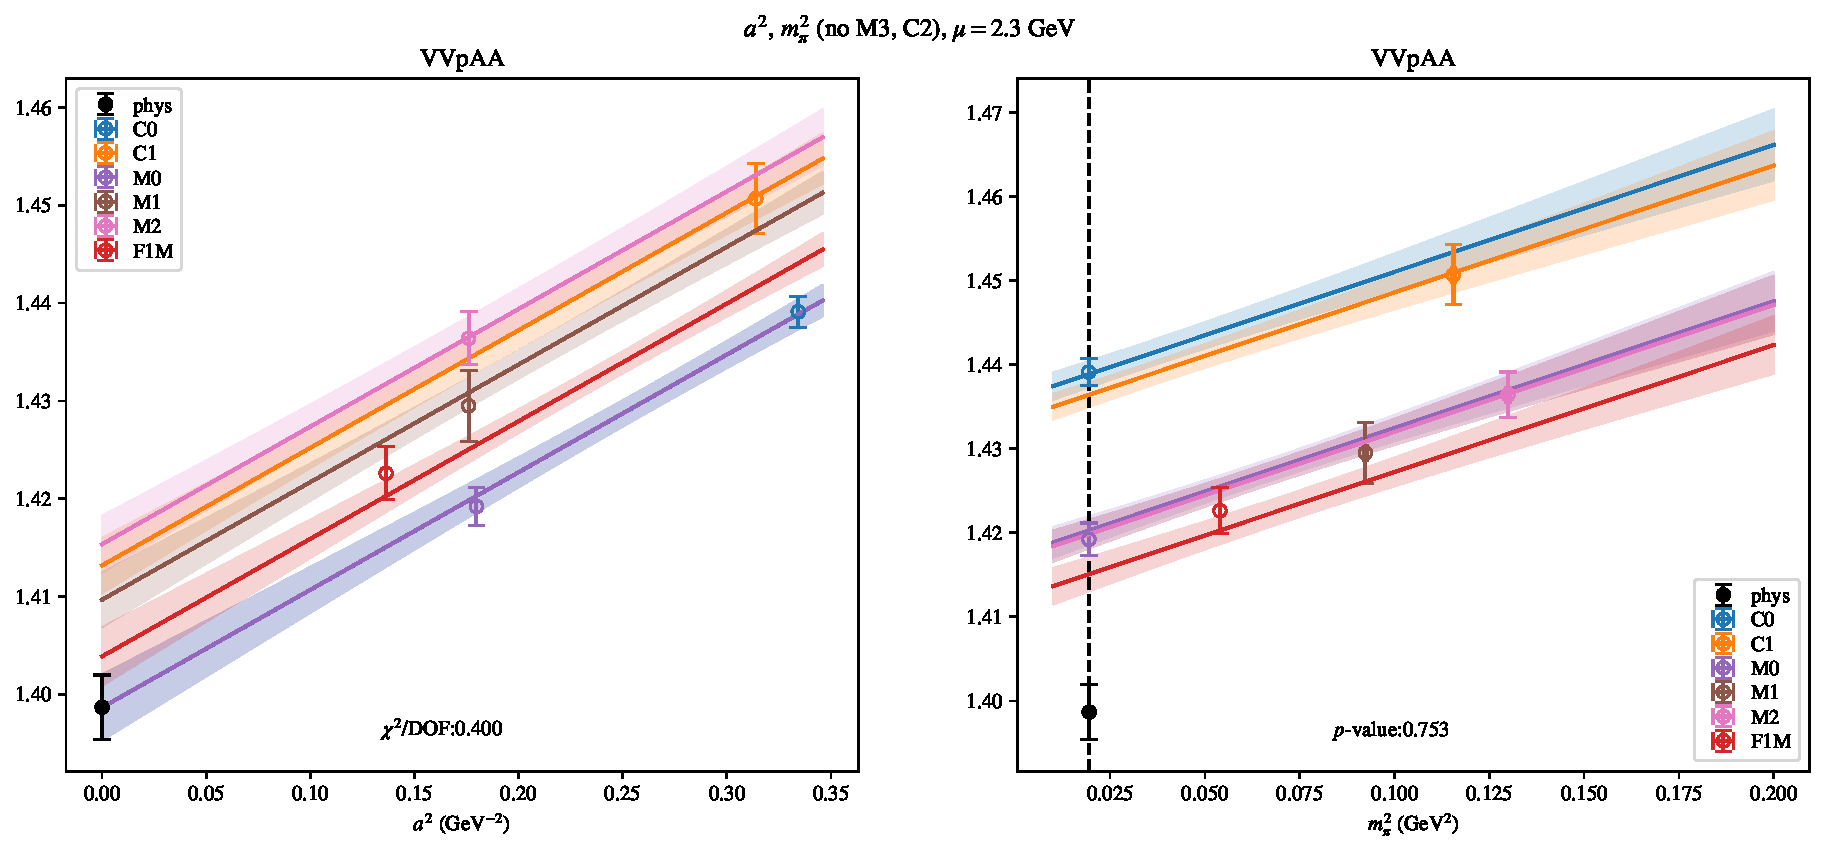
\includepdf[link, pages=-]{VVpAA/SUSY/a2m2mcut_23.pdf}
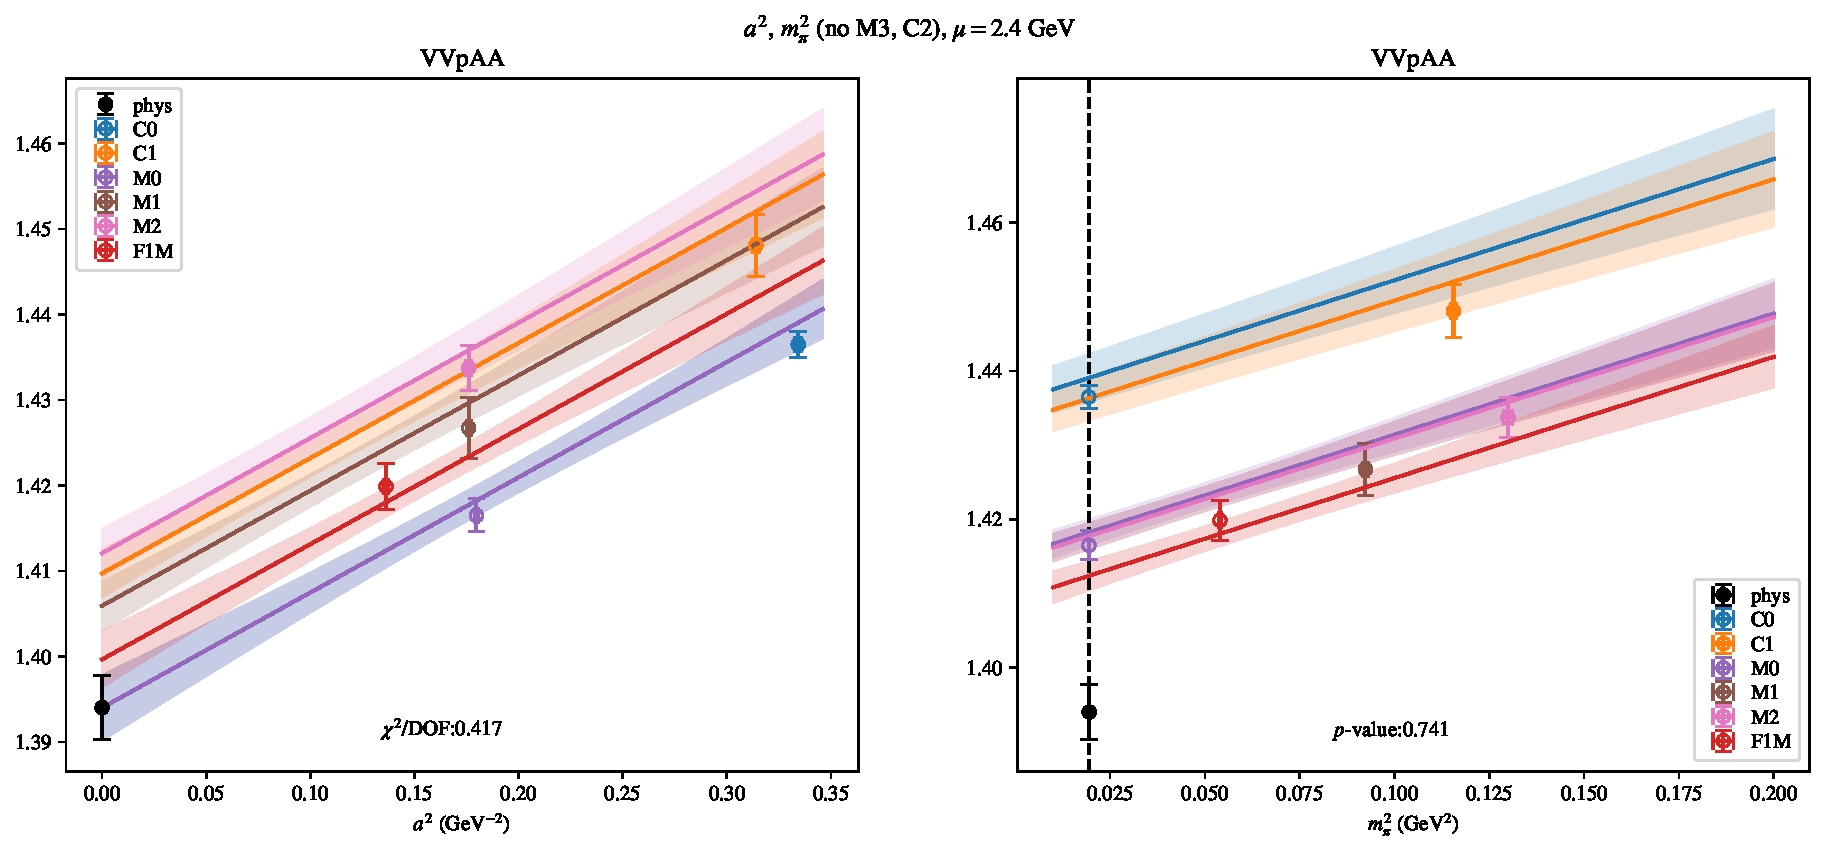
\includepdf[link, pages=-]{VVpAA/SUSY/a2m2mcut_24.pdf}
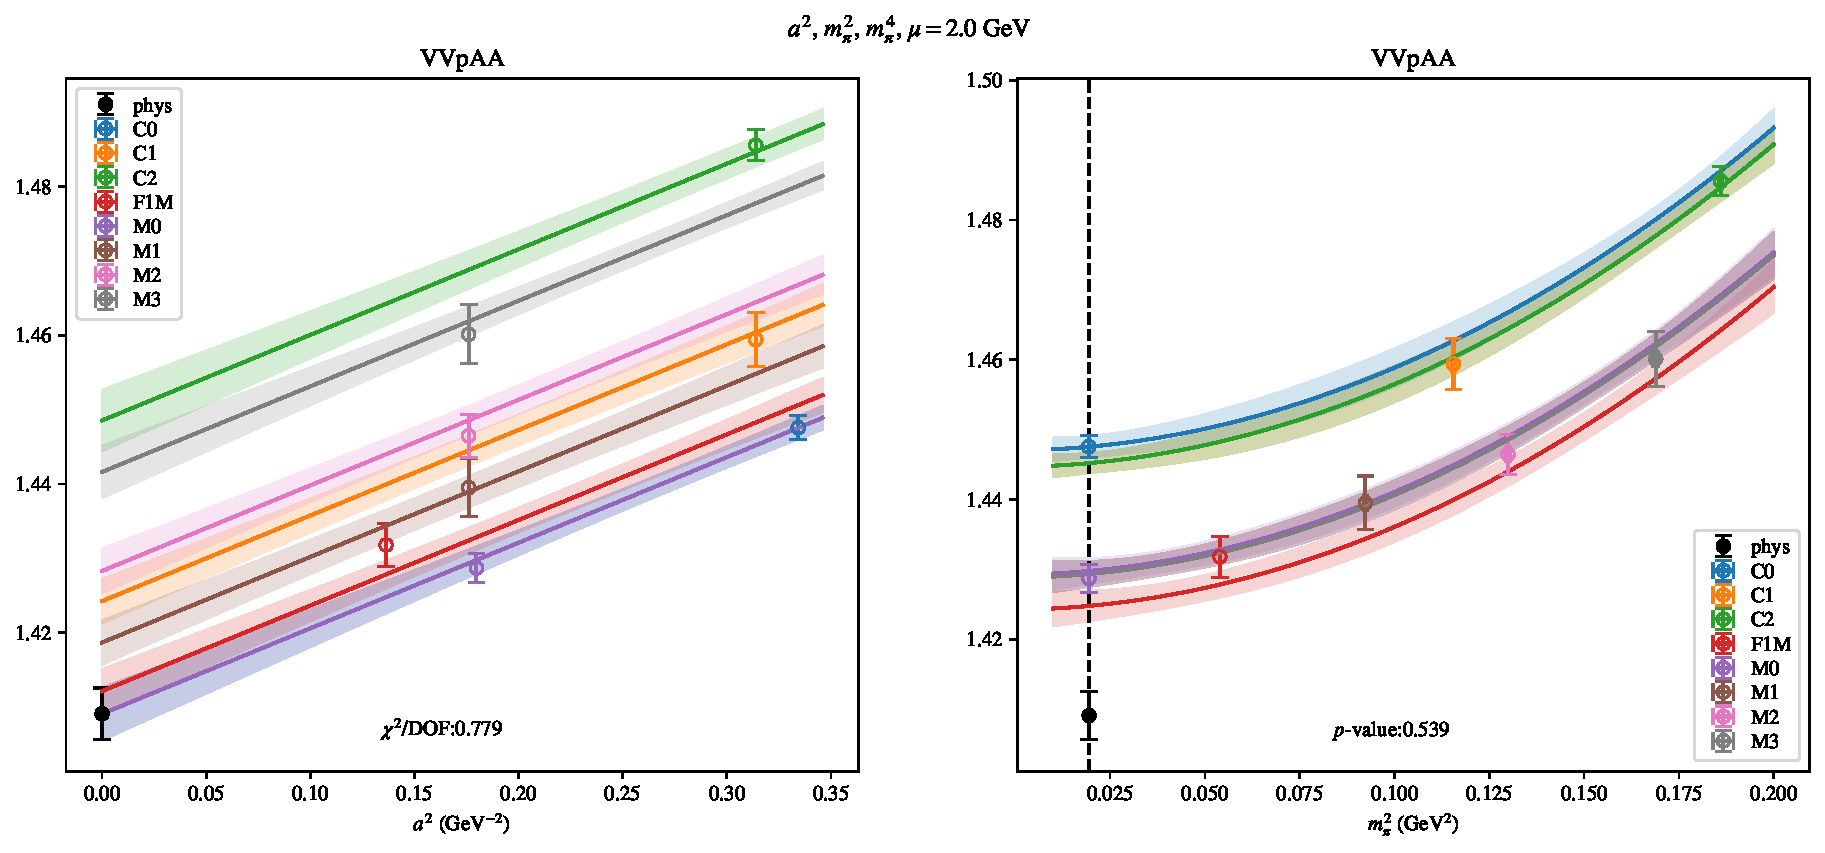
\includepdf[link, pages=-]{VVpAA/SUSY/a2m2m4_20.pdf}
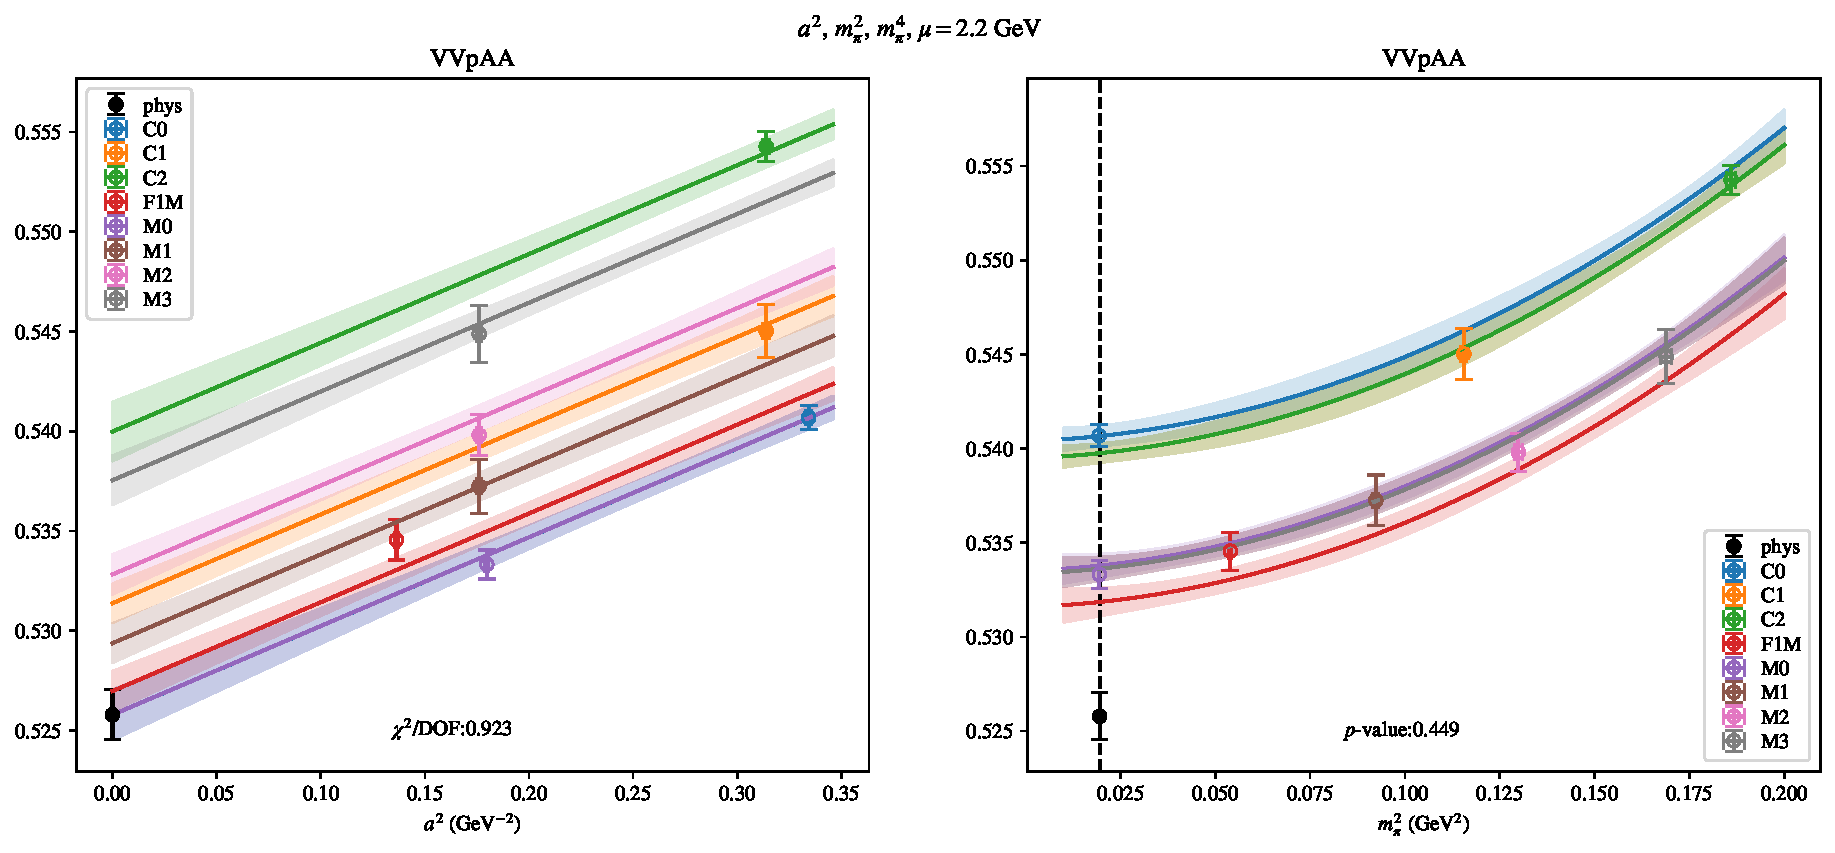
\includepdf[link, pages=-]{VVpAA/SUSY/a2m2m4_22.pdf}
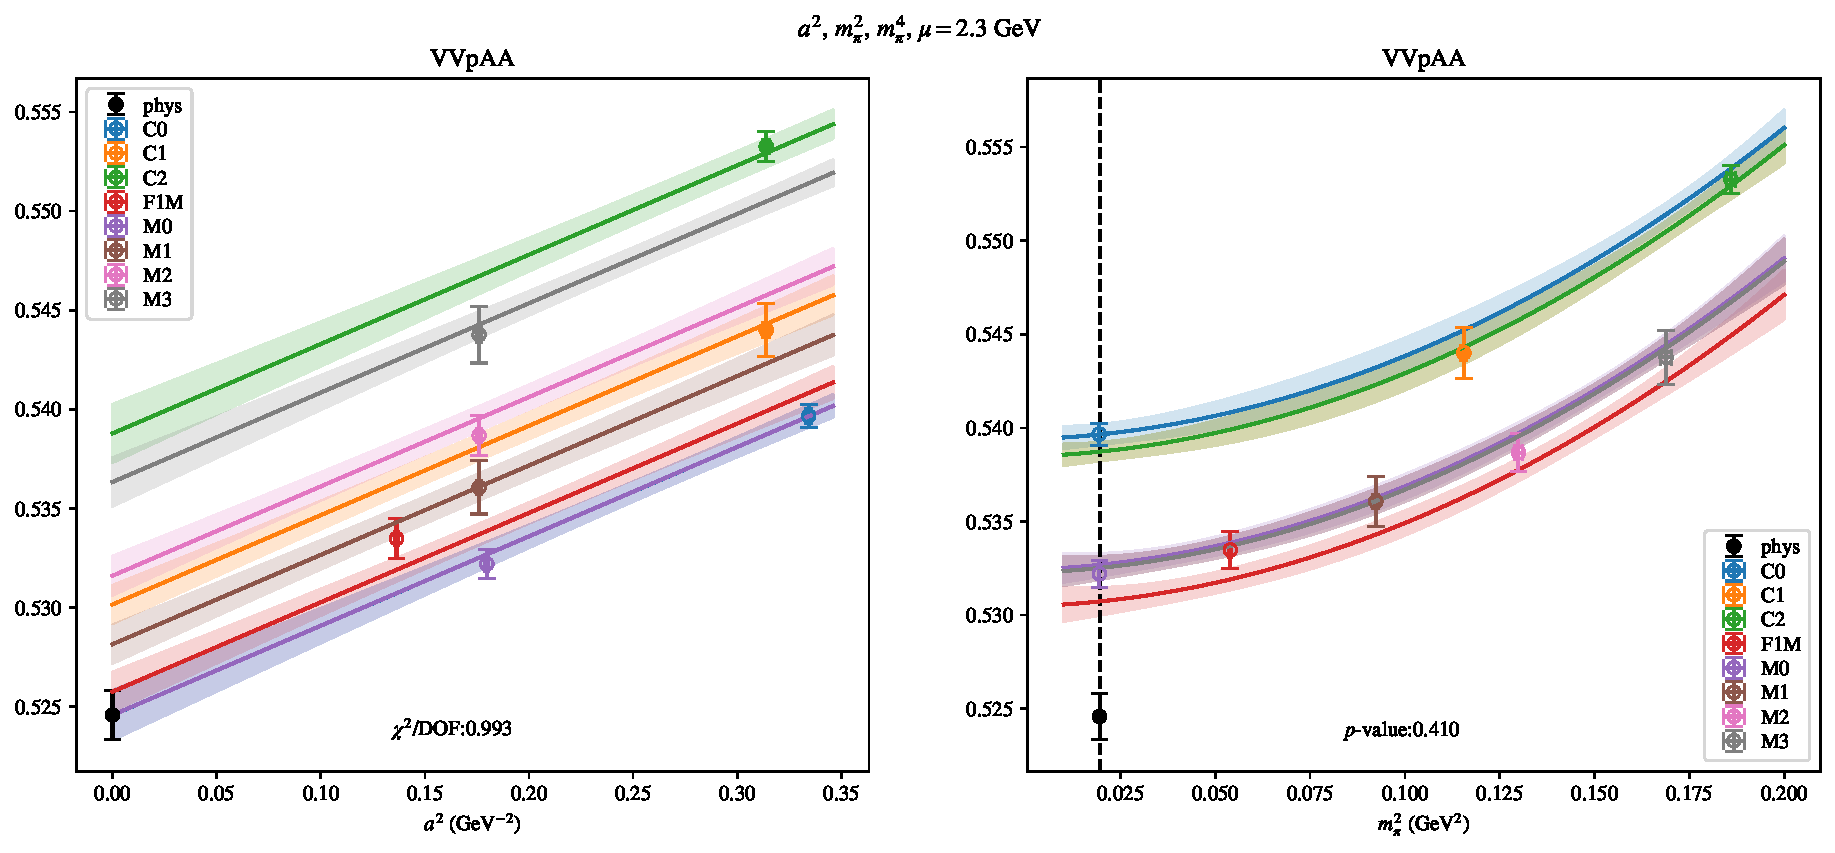
\includepdf[link, pages=-]{VVpAA/SUSY/a2m2m4_23.pdf}
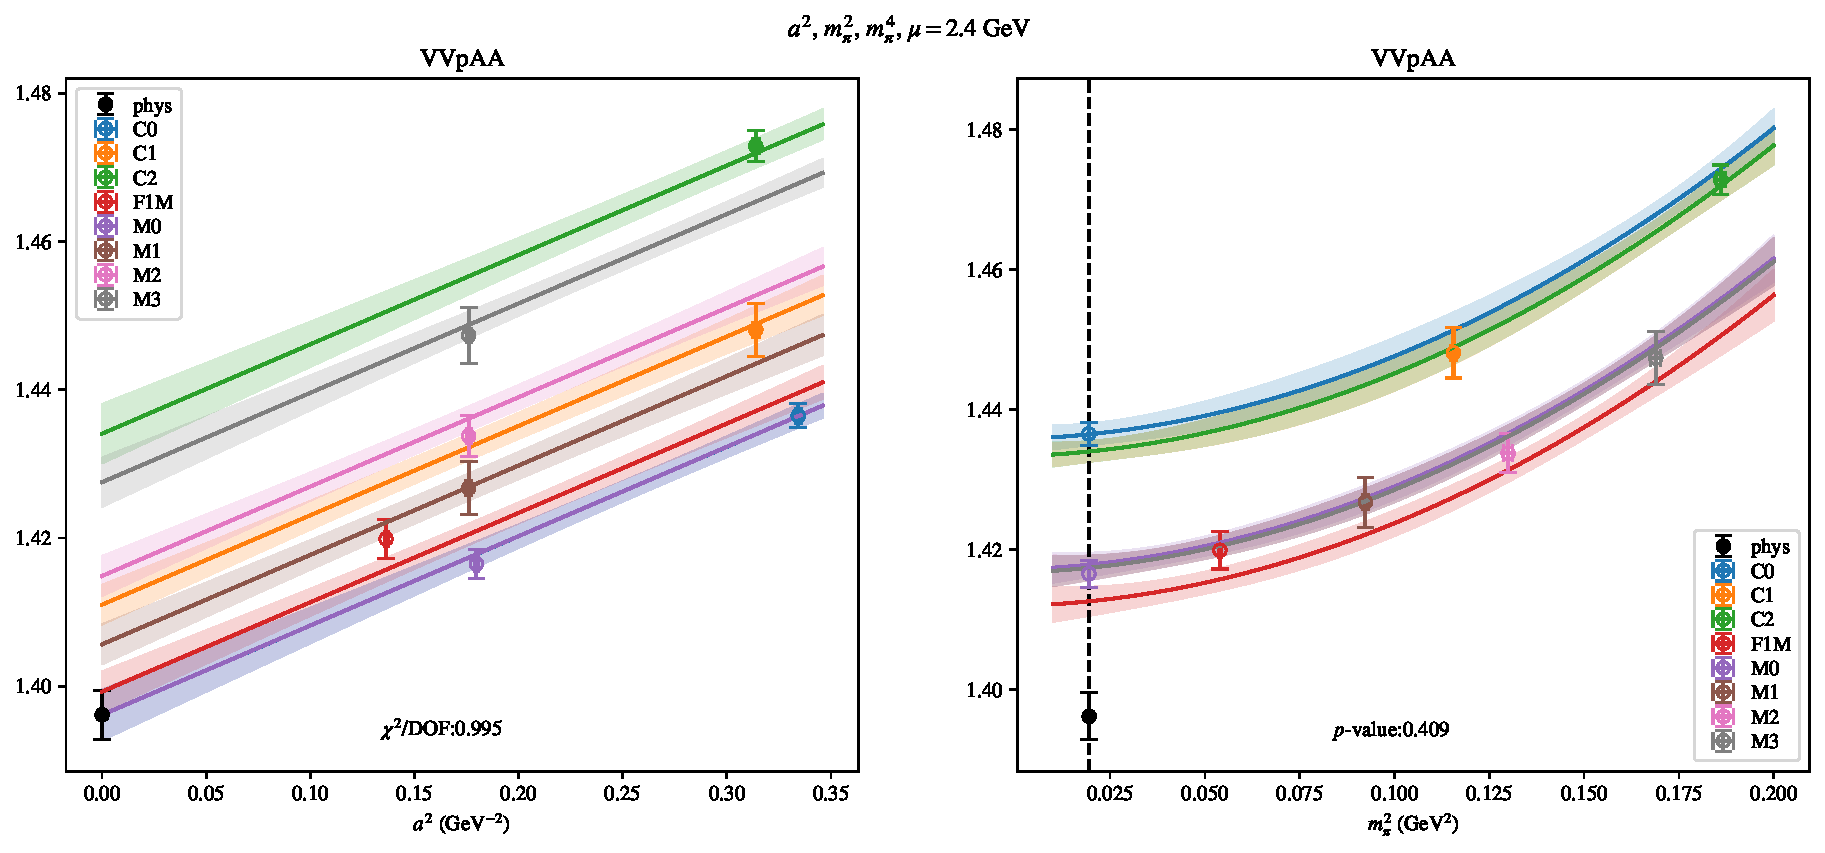
\includepdf[link, pages=-]{VVpAA/SUSY/a2m2m4_24.pdf}
\clearpage
\section{$B_2$}
\begin{table}[h!]
\begin{center}
\begin{tabular}{|c|c|c|c|c|c|}
\hline
$\mu$ (GeV) & $a^2$, $m_\pi^2$& $a^2$, $m_\pi^2$ (no C)& $a^2$, $a^4$, $m_\pi^2$& $a^2$, $m_\pi^2$ (no M3, C2)& $a^2$, $m_\pi^2$, $m_\pi^4$\\
\hline
2.0& \hyperlink{VVmAA/SUSY/a2m2_20.pdf.1}{\textbf{-0.5678(94)}: 5.086 (0.0)} & \hyperlink{VVmAA/SUSY/a2m2noC_20.pdf.1}{\textbf{-0.591(54)}: 1.037 (0.354)} & \hyperlink{VVmAA/SUSY/a2a4m2_20.pdf.1}{\textbf{-0.597(88)}: 3.569 (0.006)} & \hyperlink{VVmAA/SUSY/a2m2mcut_20.pdf.1}{\textbf{-0.567(10)}: 7.156 (0.0)} & \hyperlink{VVmAA/SUSY/a2m2m4_20.pdf.1}{\textbf{-0.566(10)}: 4.599 (0.001)}\\
2.2& \hyperlink{VVmAA/SUSY/a2m2_22.pdf.1}{\textbf{-0.5512(95)}: 5.639 (0.0)} & \hyperlink{VVmAA/SUSY/a2m2noC_22.pdf.1}{\textbf{-0.573(53)}: 1.473 (0.229)} & \hyperlink{VVmAA/SUSY/a2a4m2_22.pdf.1}{\textbf{-0.574(87)}: 5.295 (0.0)} & \hyperlink{VVmAA/SUSY/a2m2mcut_22.pdf.1}{\textbf{-0.551(10)}: 6.939 (0.0)} & \hyperlink{VVmAA/SUSY/a2m2m4_22.pdf.1}{\textbf{-0.550(10)}: 4.953 (0.001)}\\
2.3& \hyperlink{VVmAA/SUSY/a2m2_23.pdf.1}{\textbf{-0.5441(92)}: 5.563 (0.0)} & \hyperlink{VVmAA/SUSY/a2m2noC_23.pdf.1}{\textbf{-0.566(52)}: 1.564 (0.209)} & \hyperlink{VVmAA/SUSY/a2a4m2_23.pdf.1}{\textbf{-0.567(86)}: 5.126 (0.0)} & \hyperlink{VVmAA/SUSY/a2m2mcut_23.pdf.1}{\textbf{-0.5441(98)}: 7.012 (0.0)} & \hyperlink{VVmAA/SUSY/a2m2m4_23.pdf.1}{\textbf{-0.5430(98)}: 5.016 (0.0)}\\
2.4& \hyperlink{VVmAA/SUSY/a2m2_24.pdf.1}{\textbf{-0.5384(91)}: 5.522 (0.0)} & \hyperlink{VVmAA/SUSY/a2m2noC_24.pdf.1}{\textbf{-0.558(52)}: 1.48 (0.228)} & \hyperlink{VVmAA/SUSY/a2a4m2_24.pdf.1}{\textbf{-0.557(84)}: 5.677 (0.0)} & \hyperlink{VVmAA/SUSY/a2m2mcut_24.pdf.1}{\textbf{-0.5385(98)}: 7.032 (0.0)} & \hyperlink{VVmAA/SUSY/a2m2m4_24.pdf.1}{\textbf{-0.5373(97)}: 5.41 (0.0)}\\
\hline
\end{tabular}
\caption{Physical point value from chiral and continuum extrapolation at renormalisation scale $\mu$. Entries are \textbf{value(error)}: $\chi^2/\text{DOF}$ ($p$-value).}
\end{center}
\end{table}
\begin{table}[h!]
\begin{center}
\begin{tabular}{|c c|c|c|c|c|c|}
\hline
$\mu$ (GeV) &  & $a^2$, $m_\pi^2$& $a^2$, $m_\pi^2$ (no C)& $a^2$, $a^4$, $m_\pi^2$& $a^2$, $m_\pi^2$ (no M3, C2)& $a^2$, $m_\pi^2$, $m_\pi^4$\\
\hline
\multirow{2}{0.5in}{2.0} & $\alpha$ & 0.3462(68)& 0.099(54)& -0.1(13)& 0.3466(73)& 0.3539(73)\\
 & $\beta$ & 0.00789(18)& 0.00722(27)& 0.00765(18)& 0.00829(28)& 0.01015(72)\\
\hline
\multirow{2}{0.5in}{2.2} & $\alpha$ & 0.3852(74)& 0.146(55)& 0.004& 0.3844(77)& 0.3930(77)\\
 & $\beta$ & 0.00760(15)& 0.00685(24)& 0.00742(16)& 0.00811(28)& 0.01000(76)\\
\hline
\multirow{2}{0.5in}{2.3} & $\alpha$ & 0.4059(74)& 0.167(55)& 0.022& 0.4051(78)& 0.4134(78)\\
 & $\beta$ & 0.00756(15)& 0.00682(24)& 0.00738(16)& 0.00801(27)& 0.00982(75)\\
\hline
\multirow{2}{0.5in}{2.4} & $\alpha$ & 0.4220(74)& 0.205(55)& 0.10(13)& 0.4202(79)& 0.4289(79)\\
 & $\beta$ & 0.00757(14)& 0.00680(22)& 0.00743(15)& 0.00793(25)& 0.00949(71)\\
\hline
\end{tabular}
\caption{Fit values of coefficients in $B = B_{phys} + \mathbf{\alpha} a^2 + \mathbf{\beta}\left(\frac{m_\pi^2}{f_\pi^2}-\frac{m_{\pi,PDG}^2}{f_\pi^2}\right) + \ldots$.}
\end{center}
\end{table}
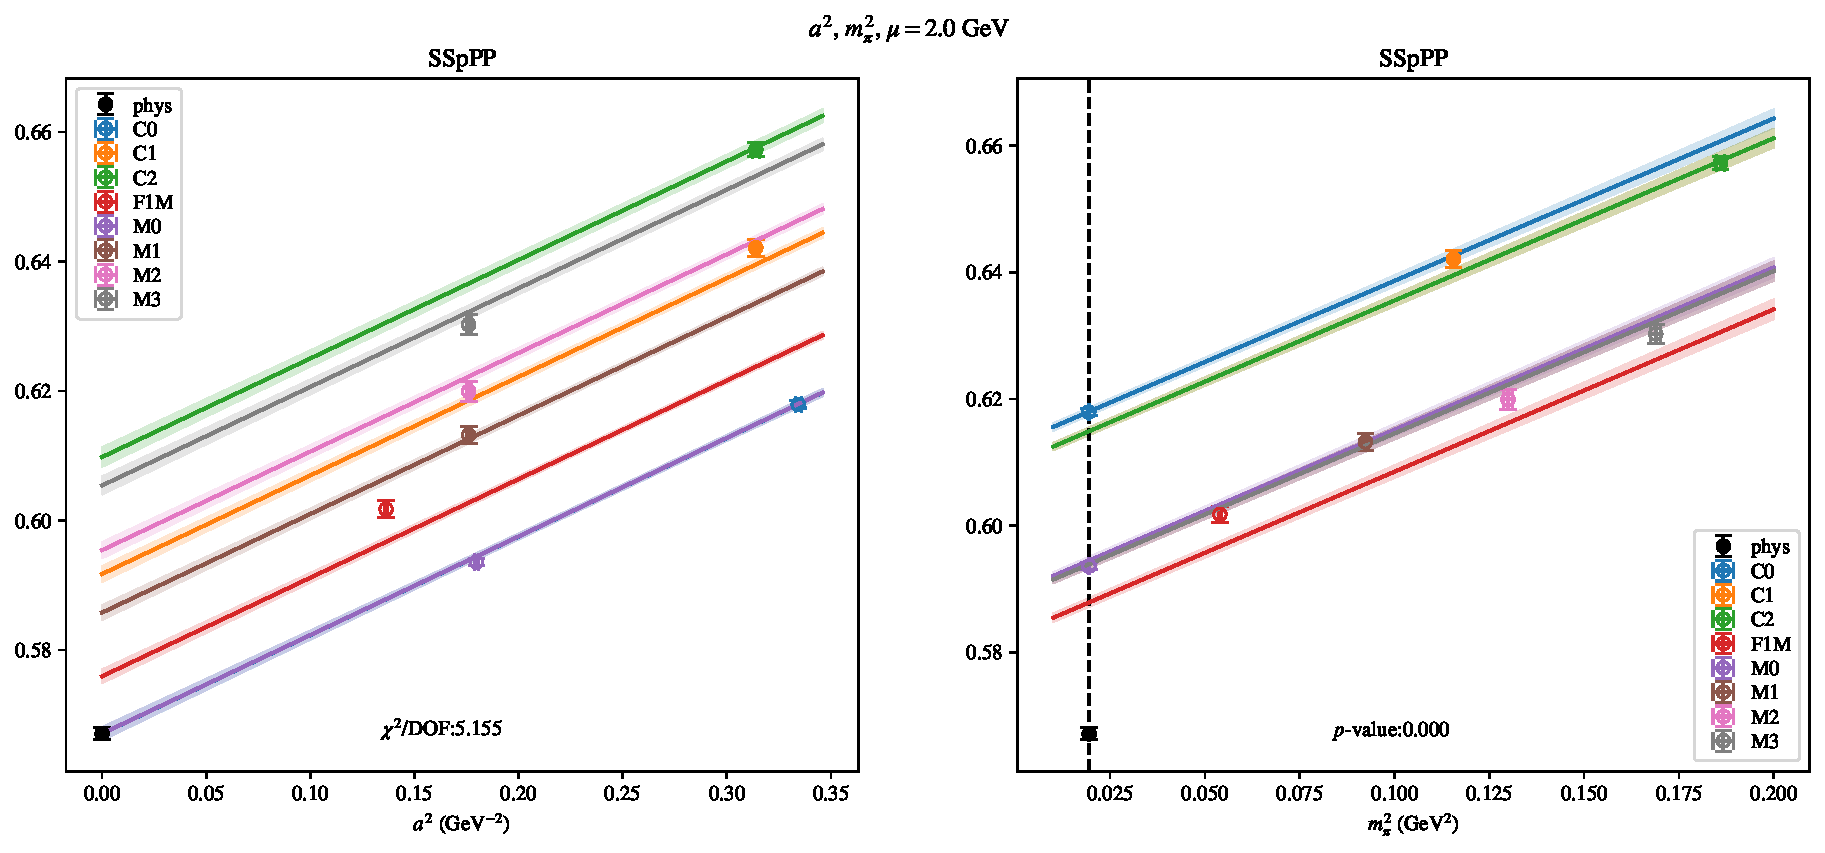
\includepdf[link, pages=-]{VVmAA/SUSY/a2m2_20.pdf}
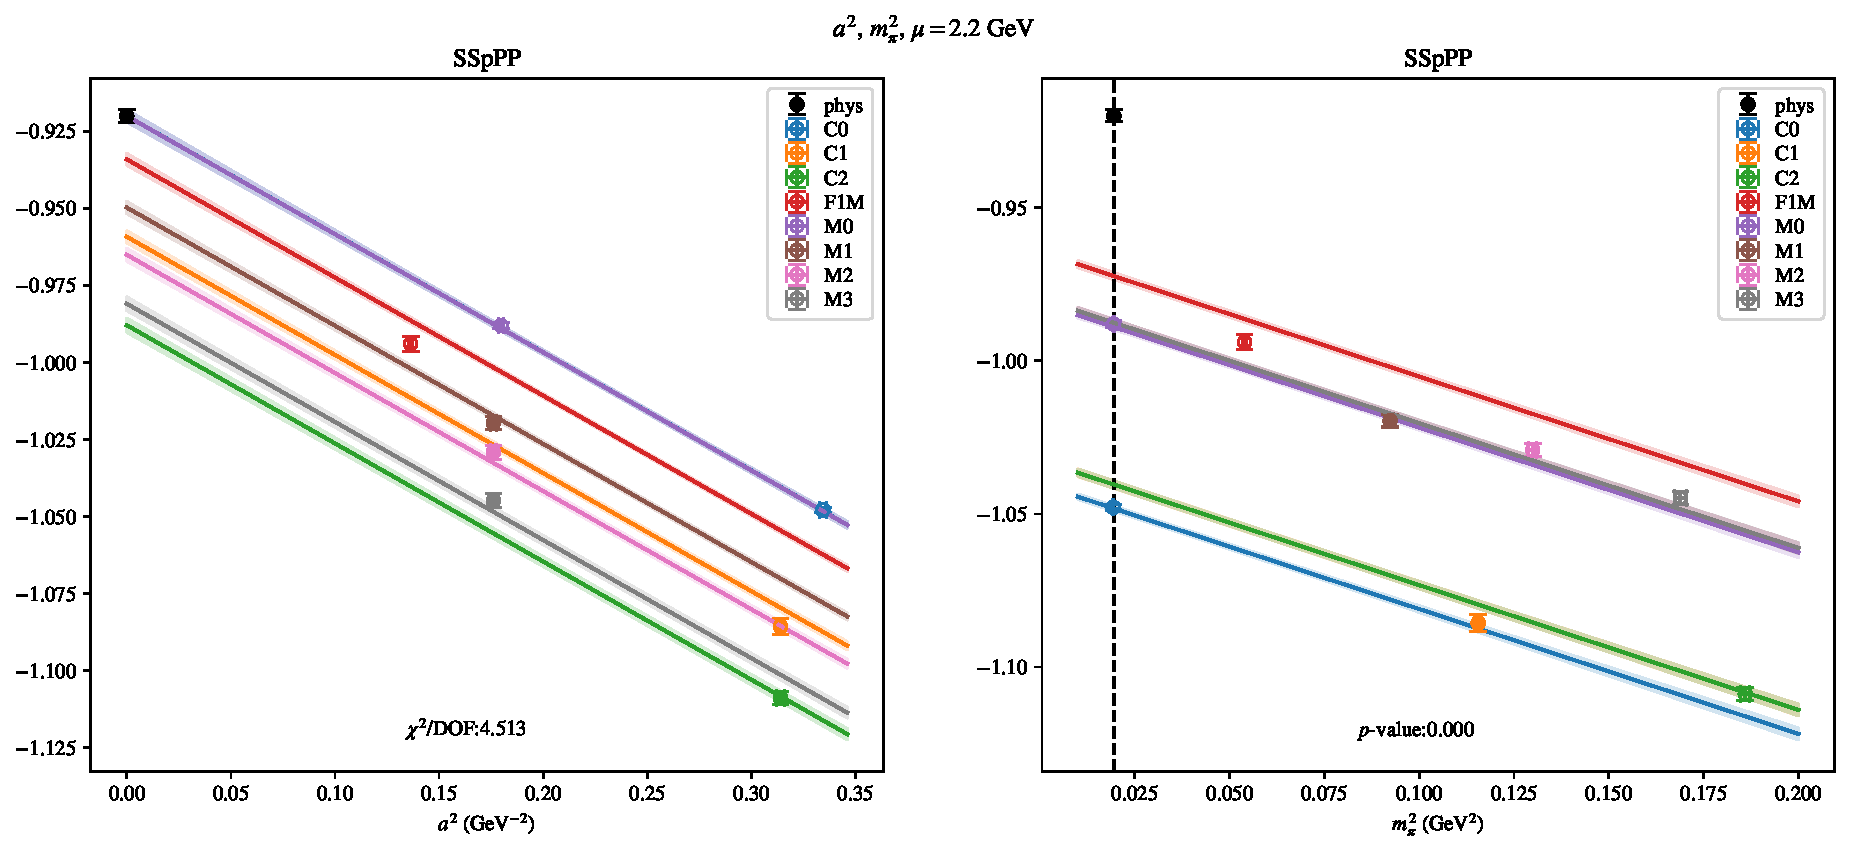
\includepdf[link, pages=-]{VVmAA/SUSY/a2m2_22.pdf}
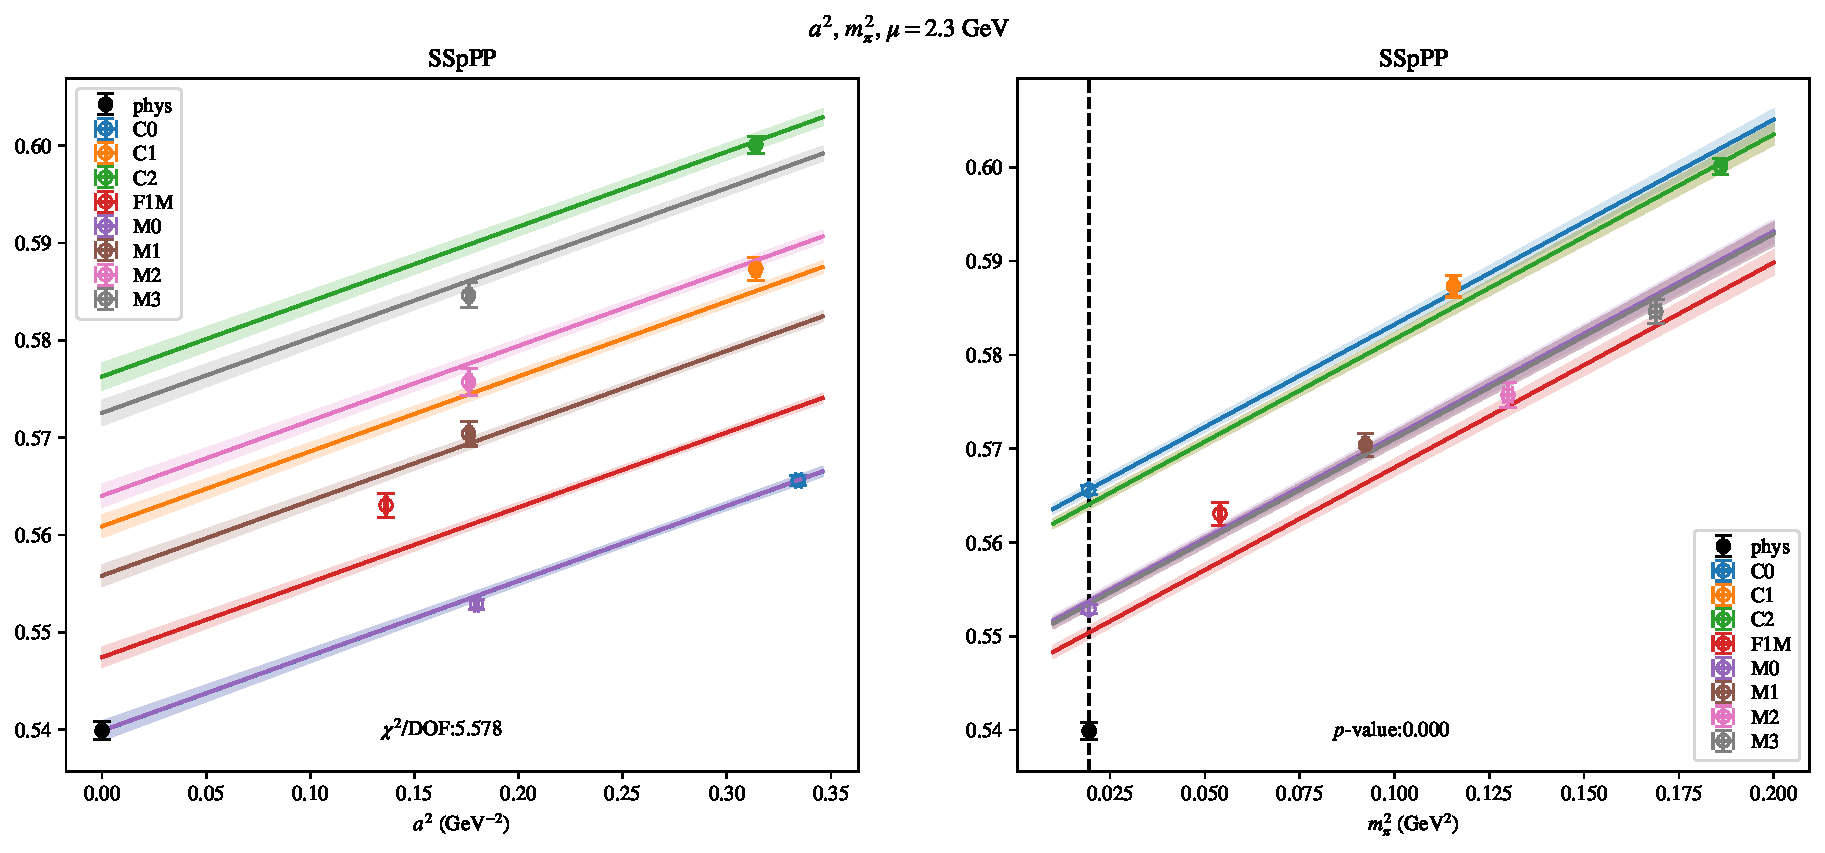
\includepdf[link, pages=-]{VVmAA/SUSY/a2m2_23.pdf}
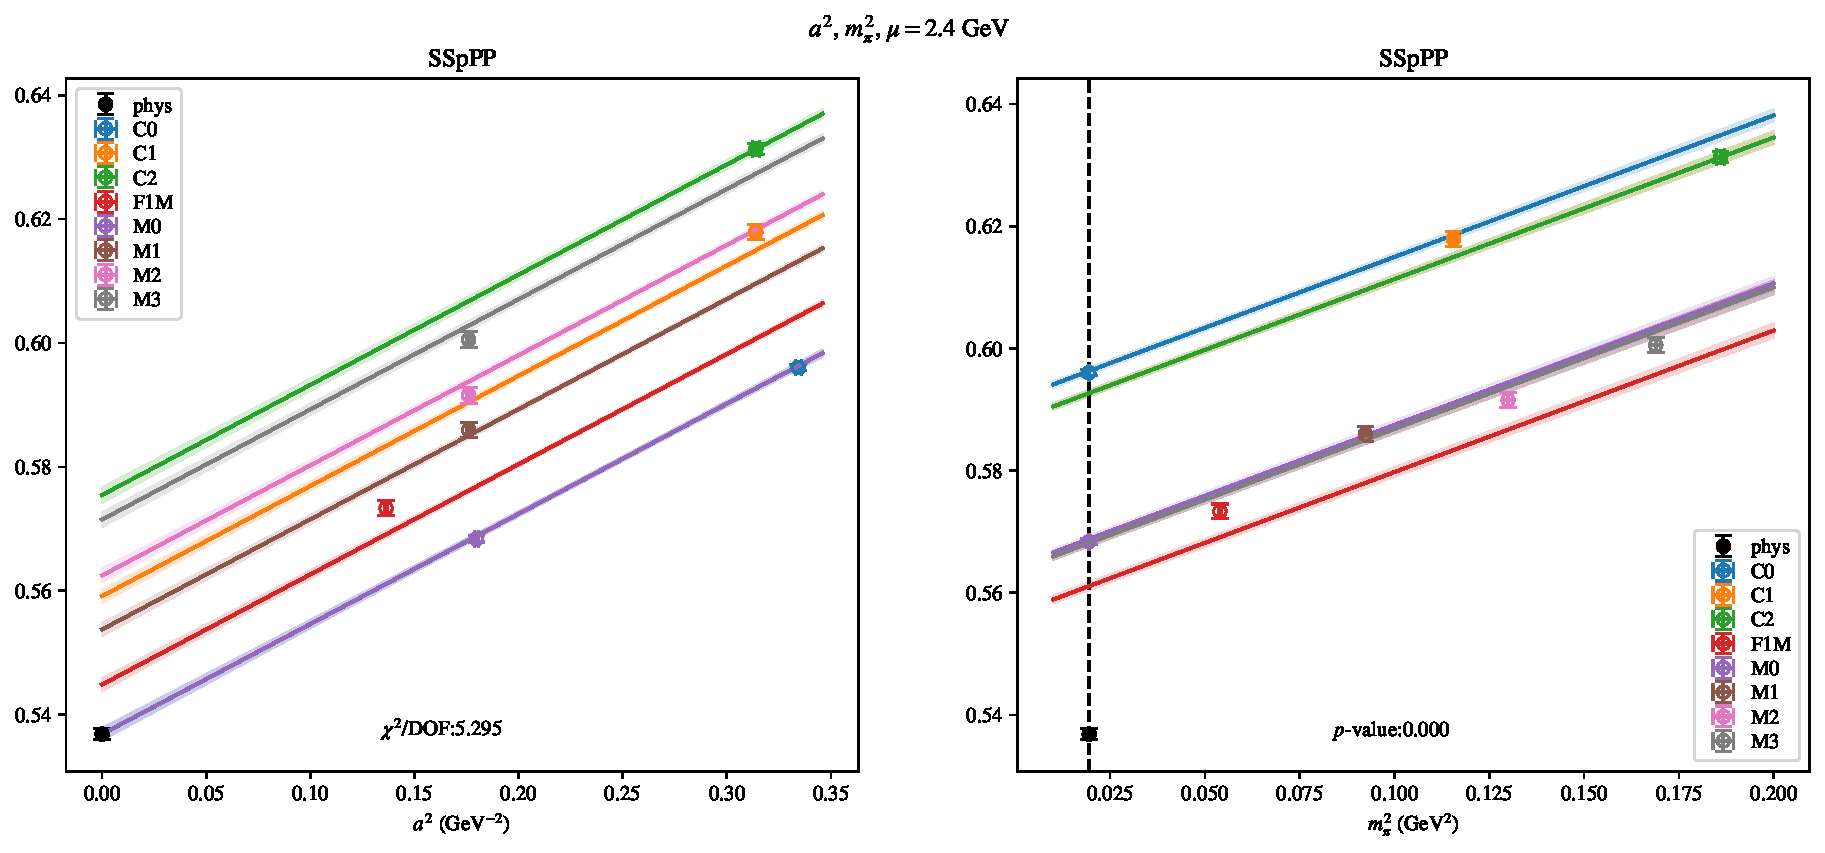
\includepdf[link, pages=-]{VVmAA/SUSY/a2m2_24.pdf}
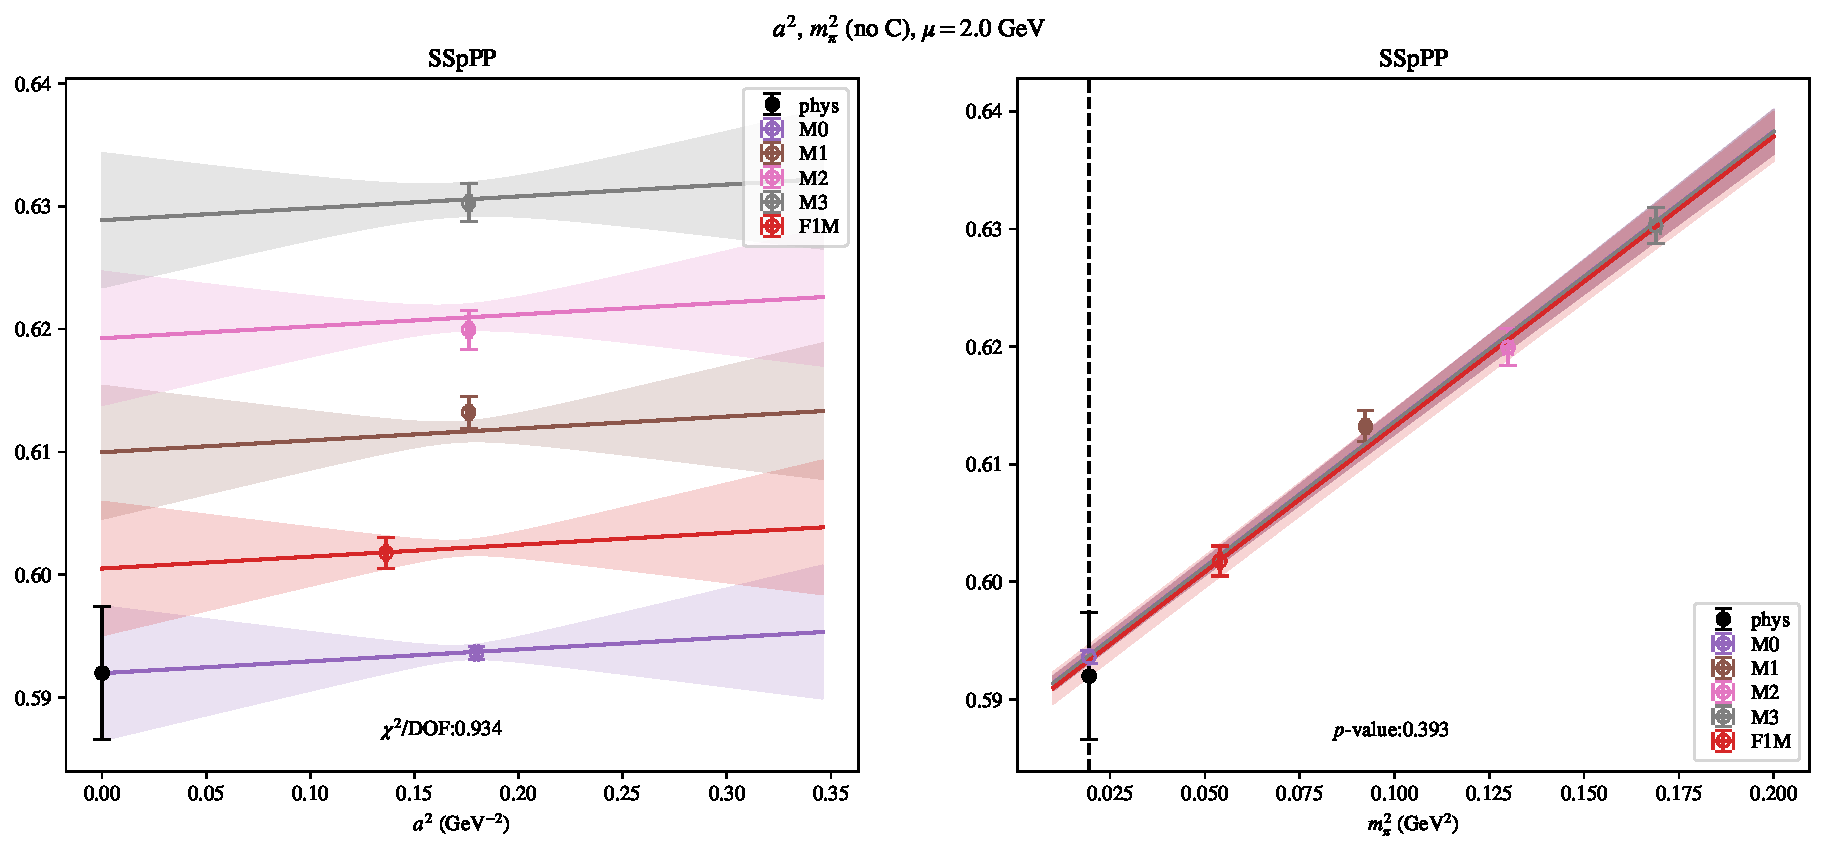
\includepdf[link, pages=-]{VVmAA/SUSY/a2m2noC_20.pdf}
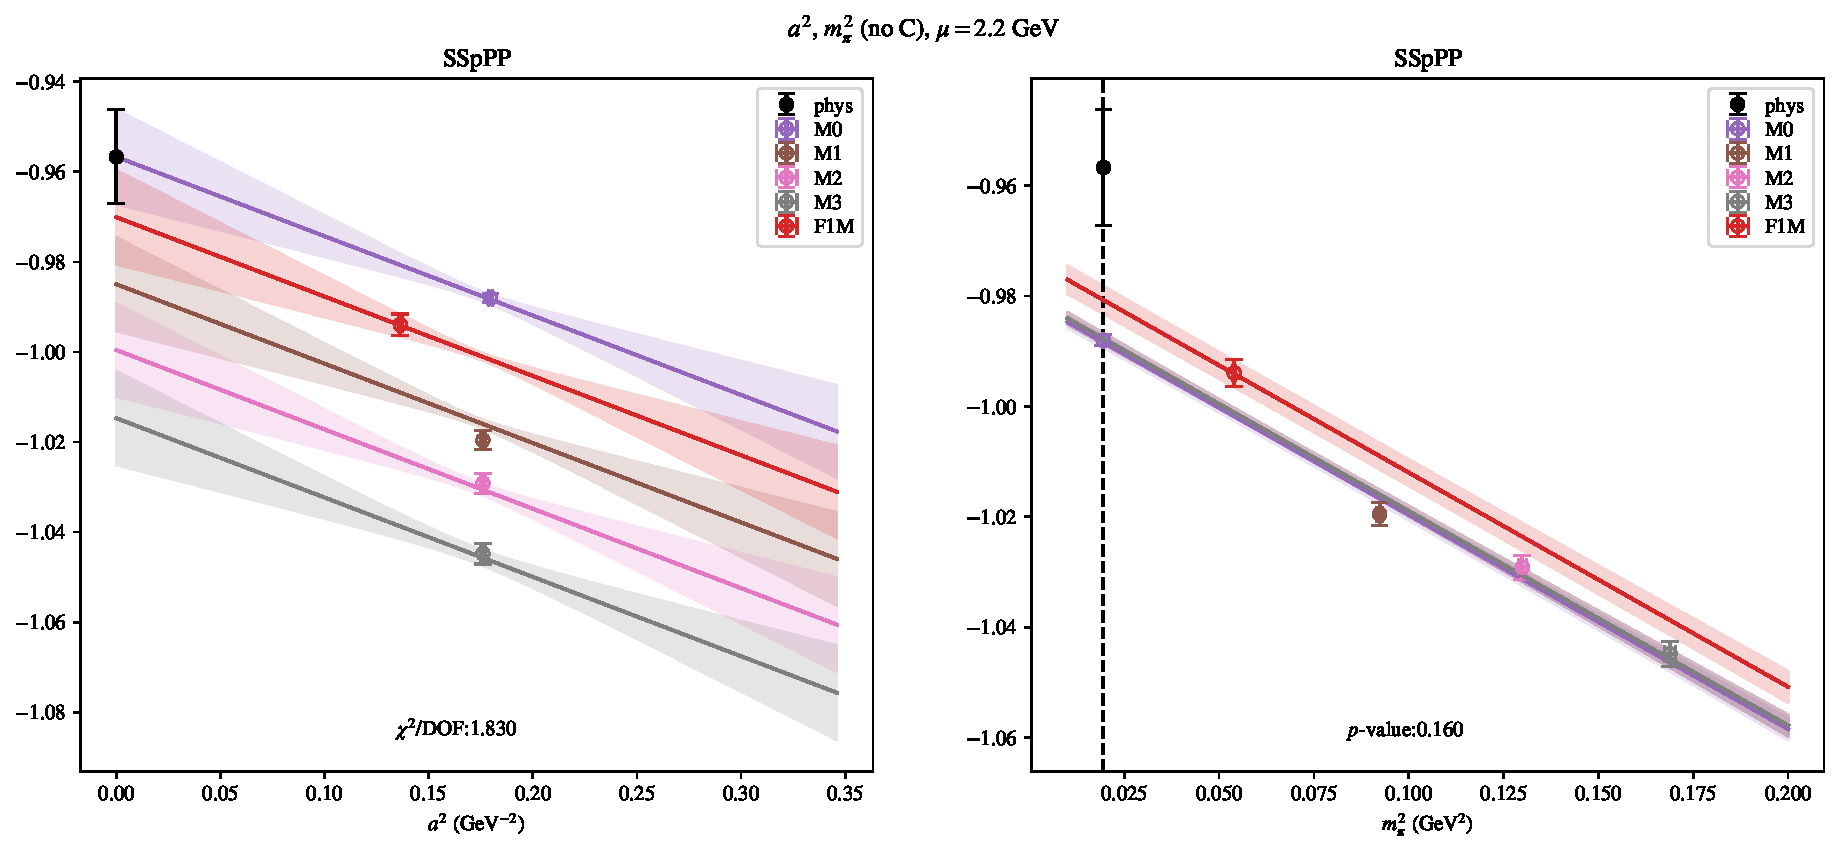
\includepdf[link, pages=-]{VVmAA/SUSY/a2m2noC_22.pdf}
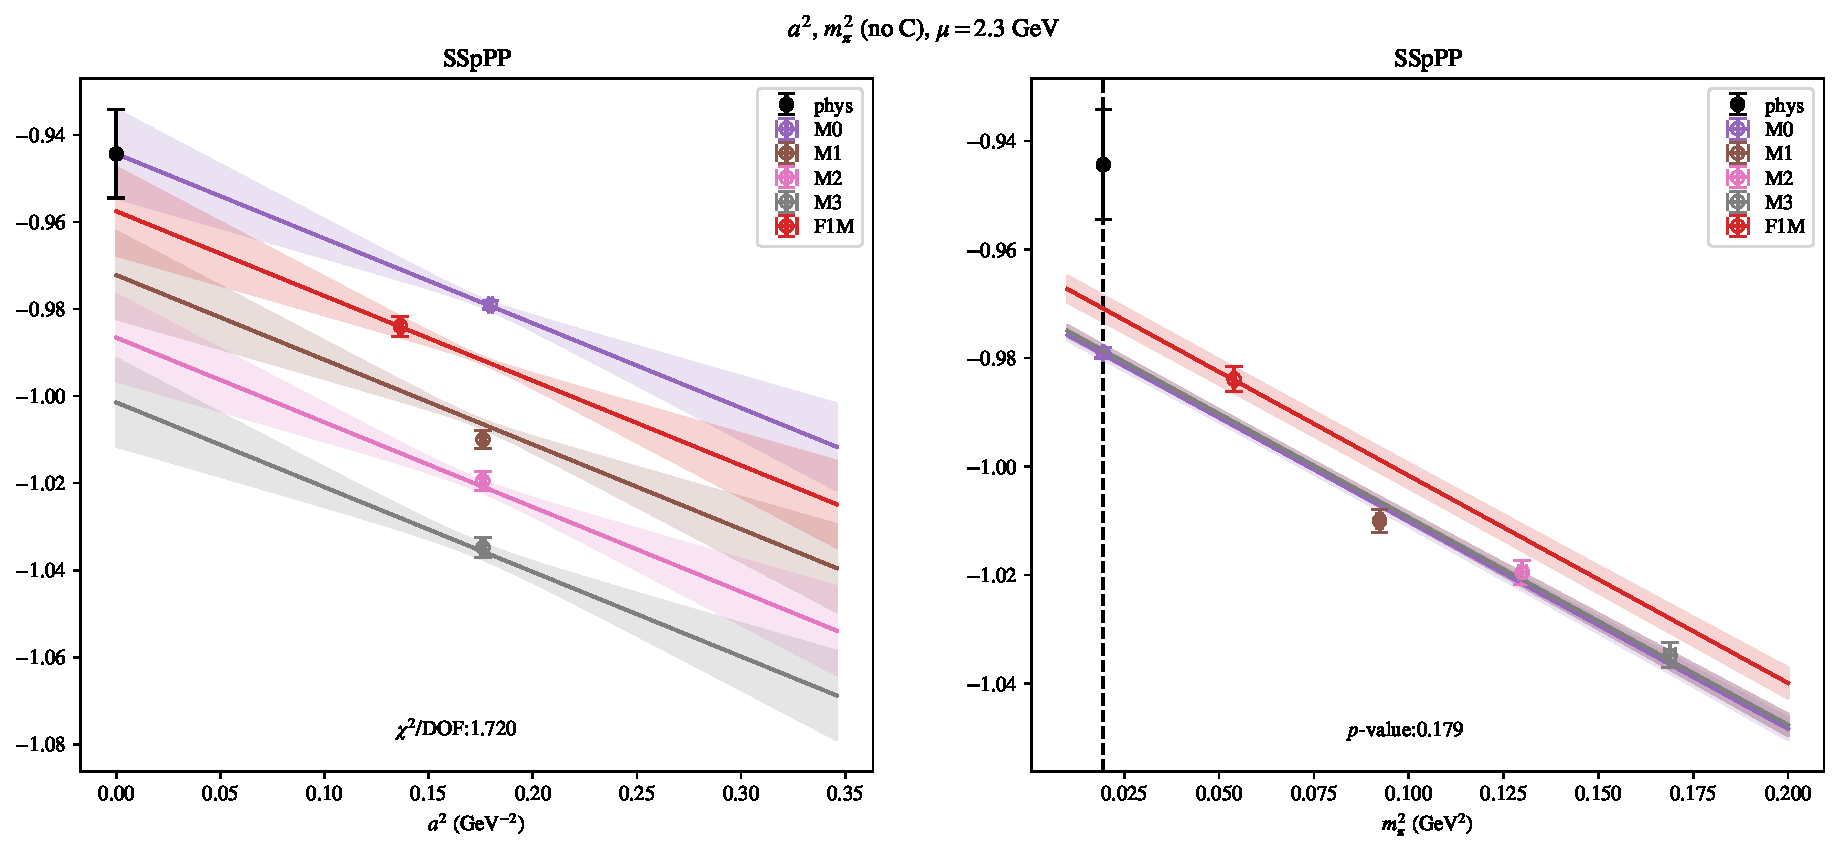
\includepdf[link, pages=-]{VVmAA/SUSY/a2m2noC_23.pdf}
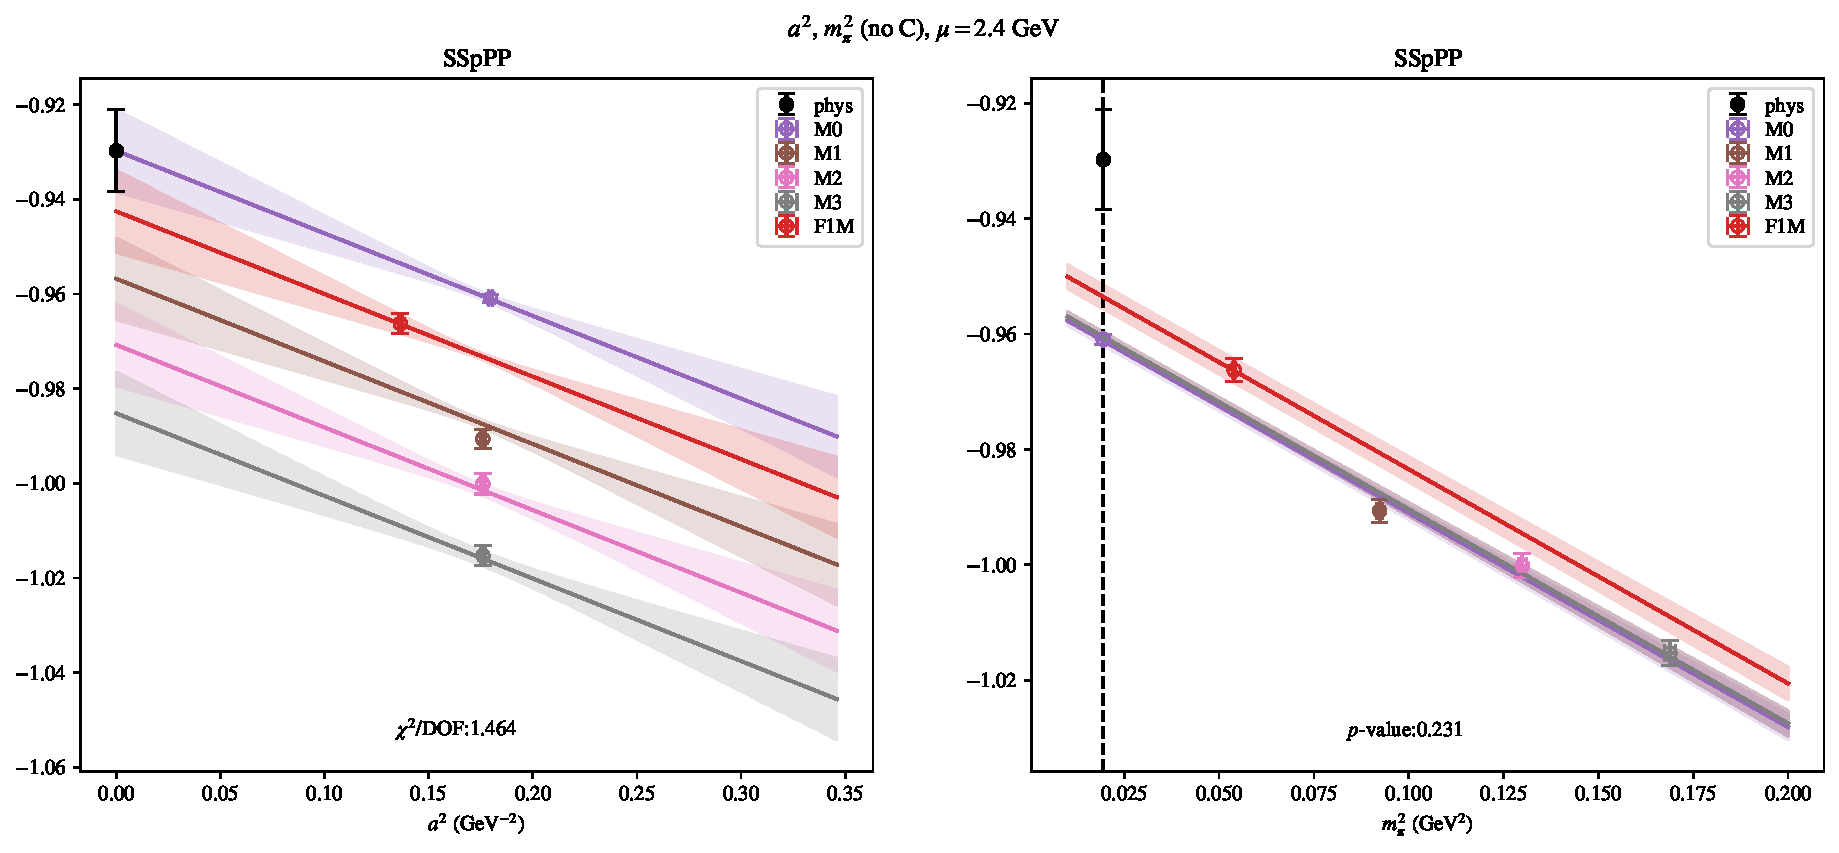
\includepdf[link, pages=-]{VVmAA/SUSY/a2m2noC_24.pdf}
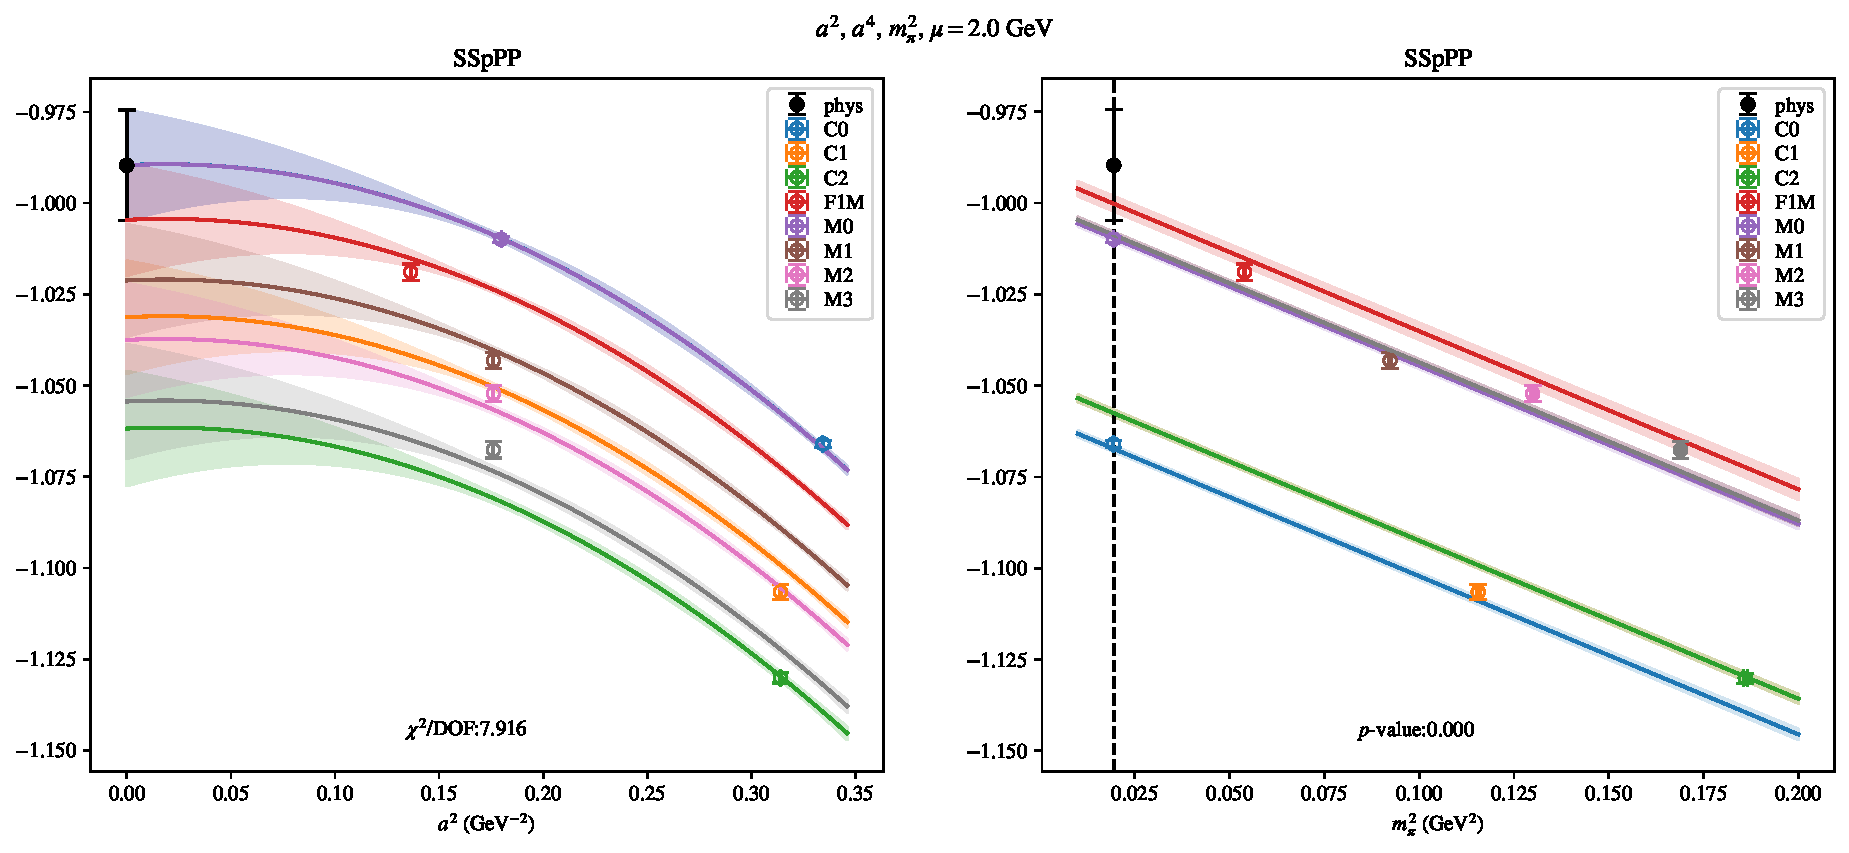
\includepdf[link, pages=-]{VVmAA/SUSY/a2a4m2_20.pdf}
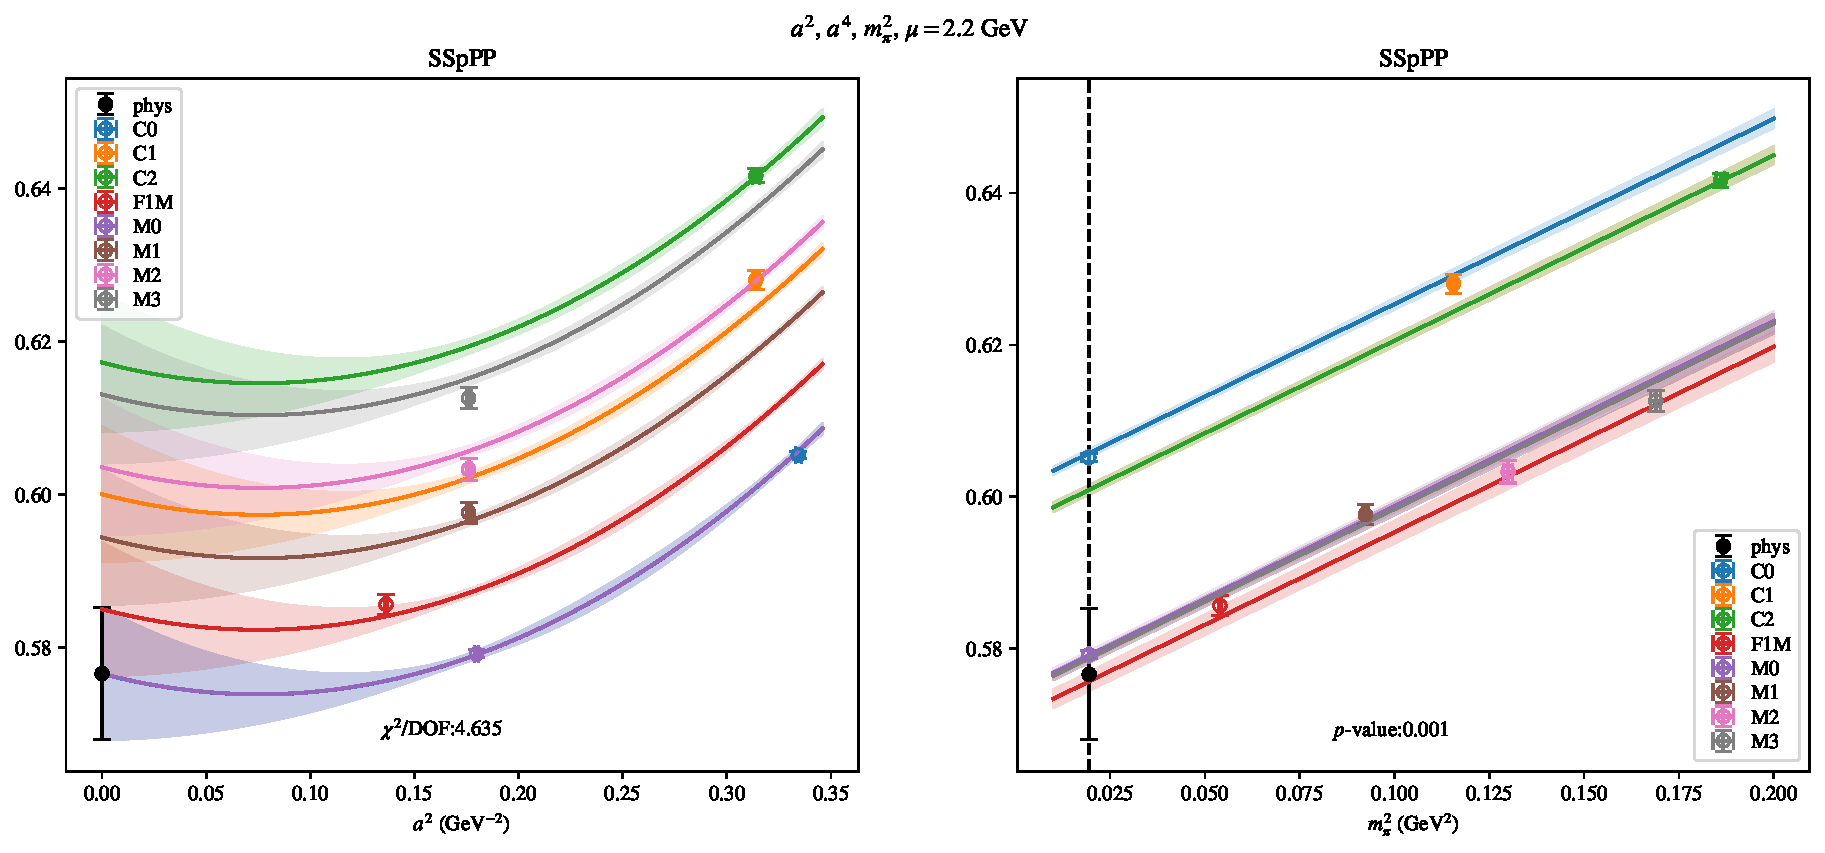
\includepdf[link, pages=-]{VVmAA/SUSY/a2a4m2_22.pdf}
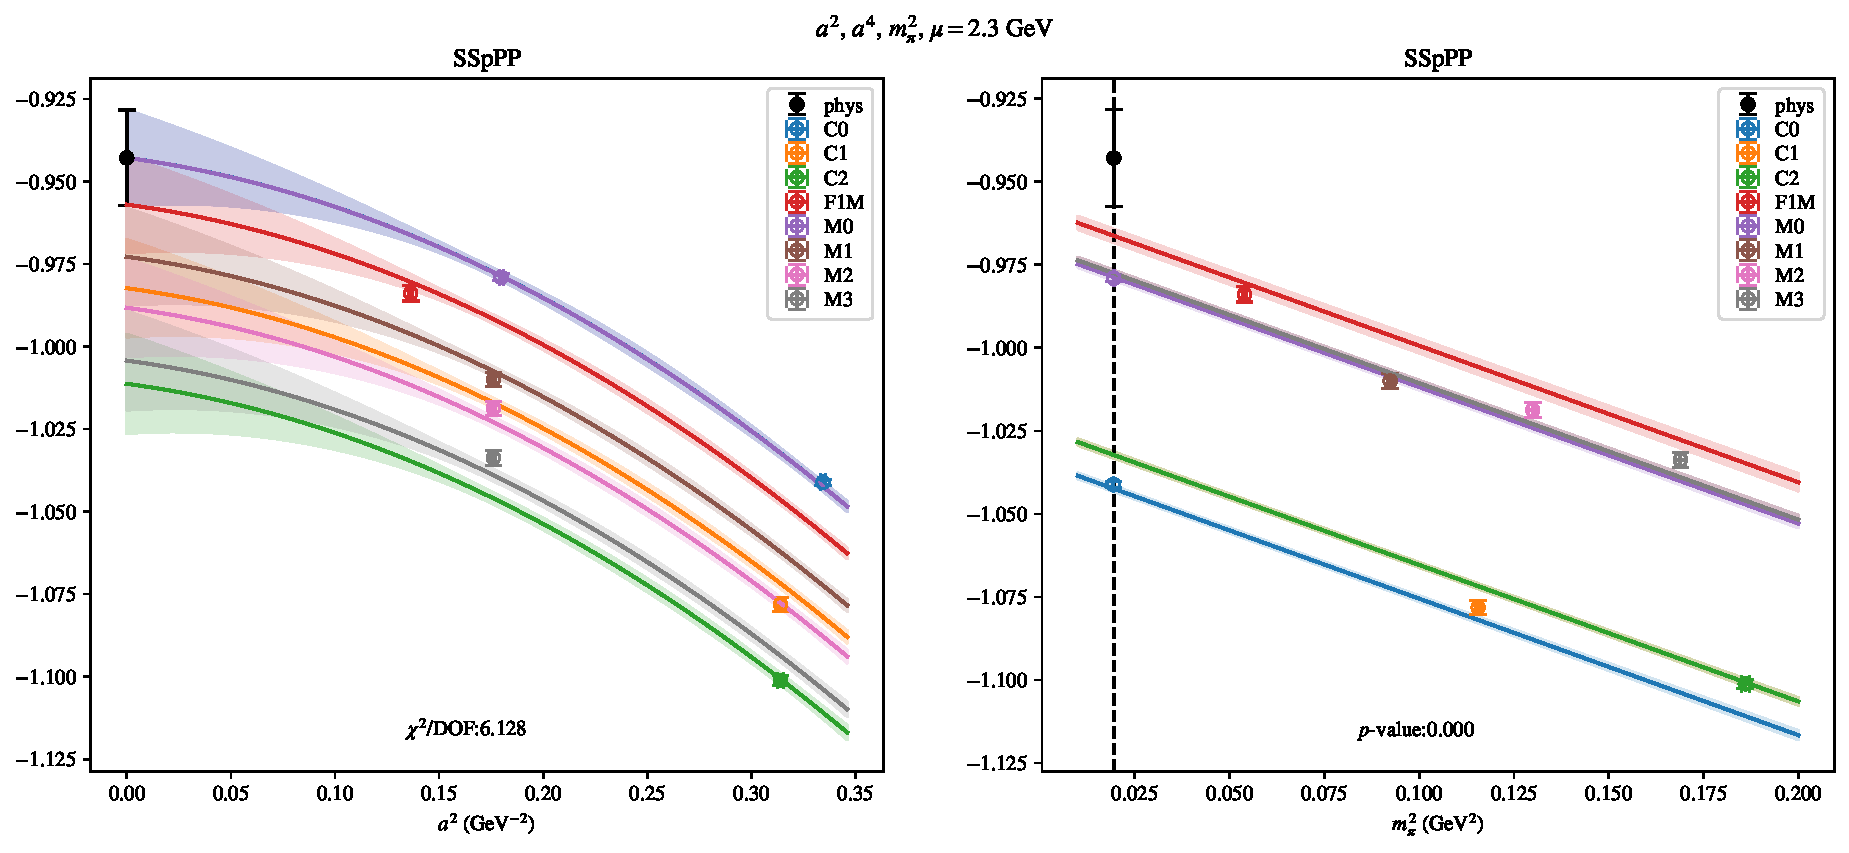
\includepdf[link, pages=-]{VVmAA/SUSY/a2a4m2_23.pdf}
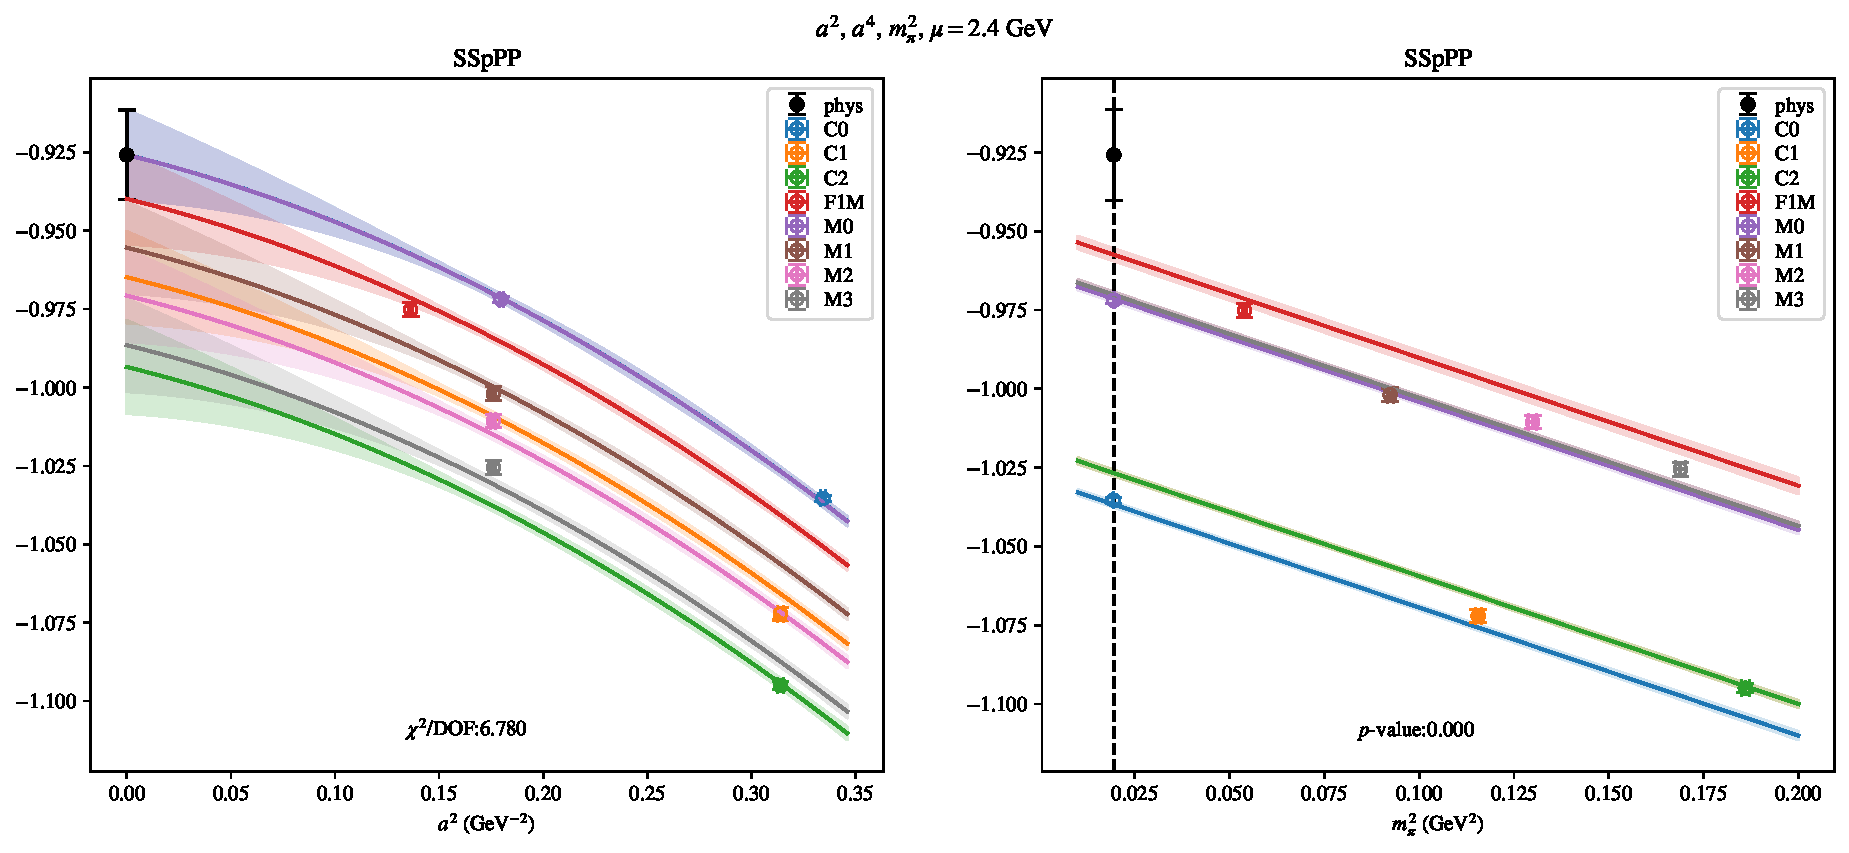
\includepdf[link, pages=-]{VVmAA/SUSY/a2a4m2_24.pdf}
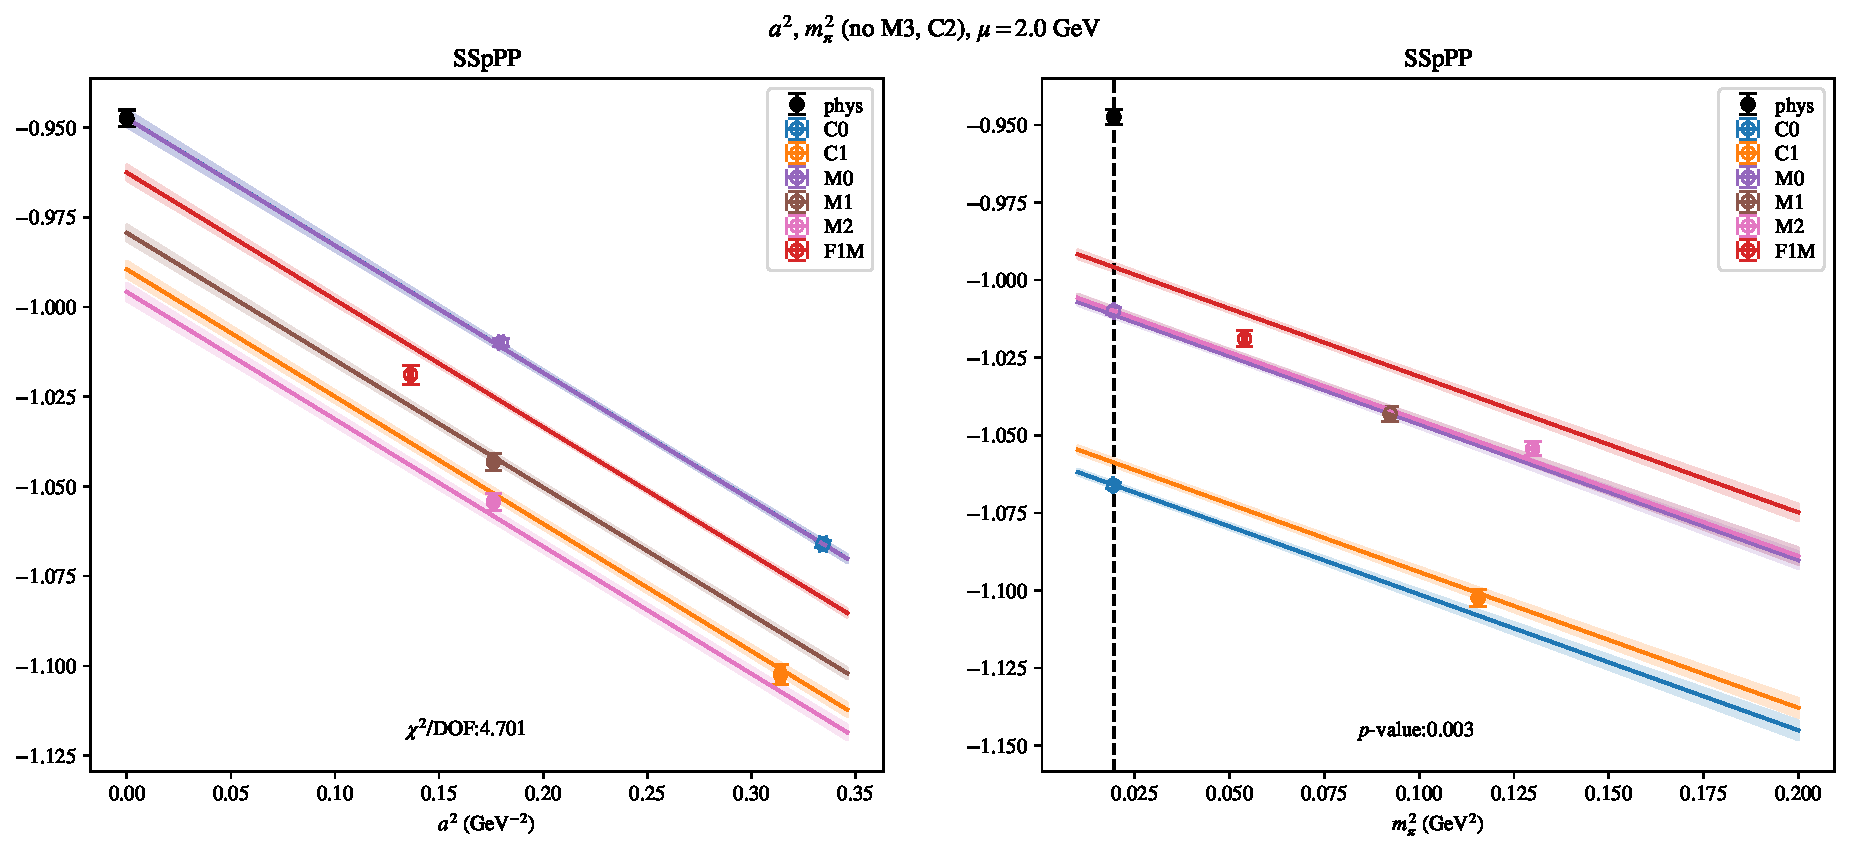
\includepdf[link, pages=-]{VVmAA/SUSY/a2m2mcut_20.pdf}
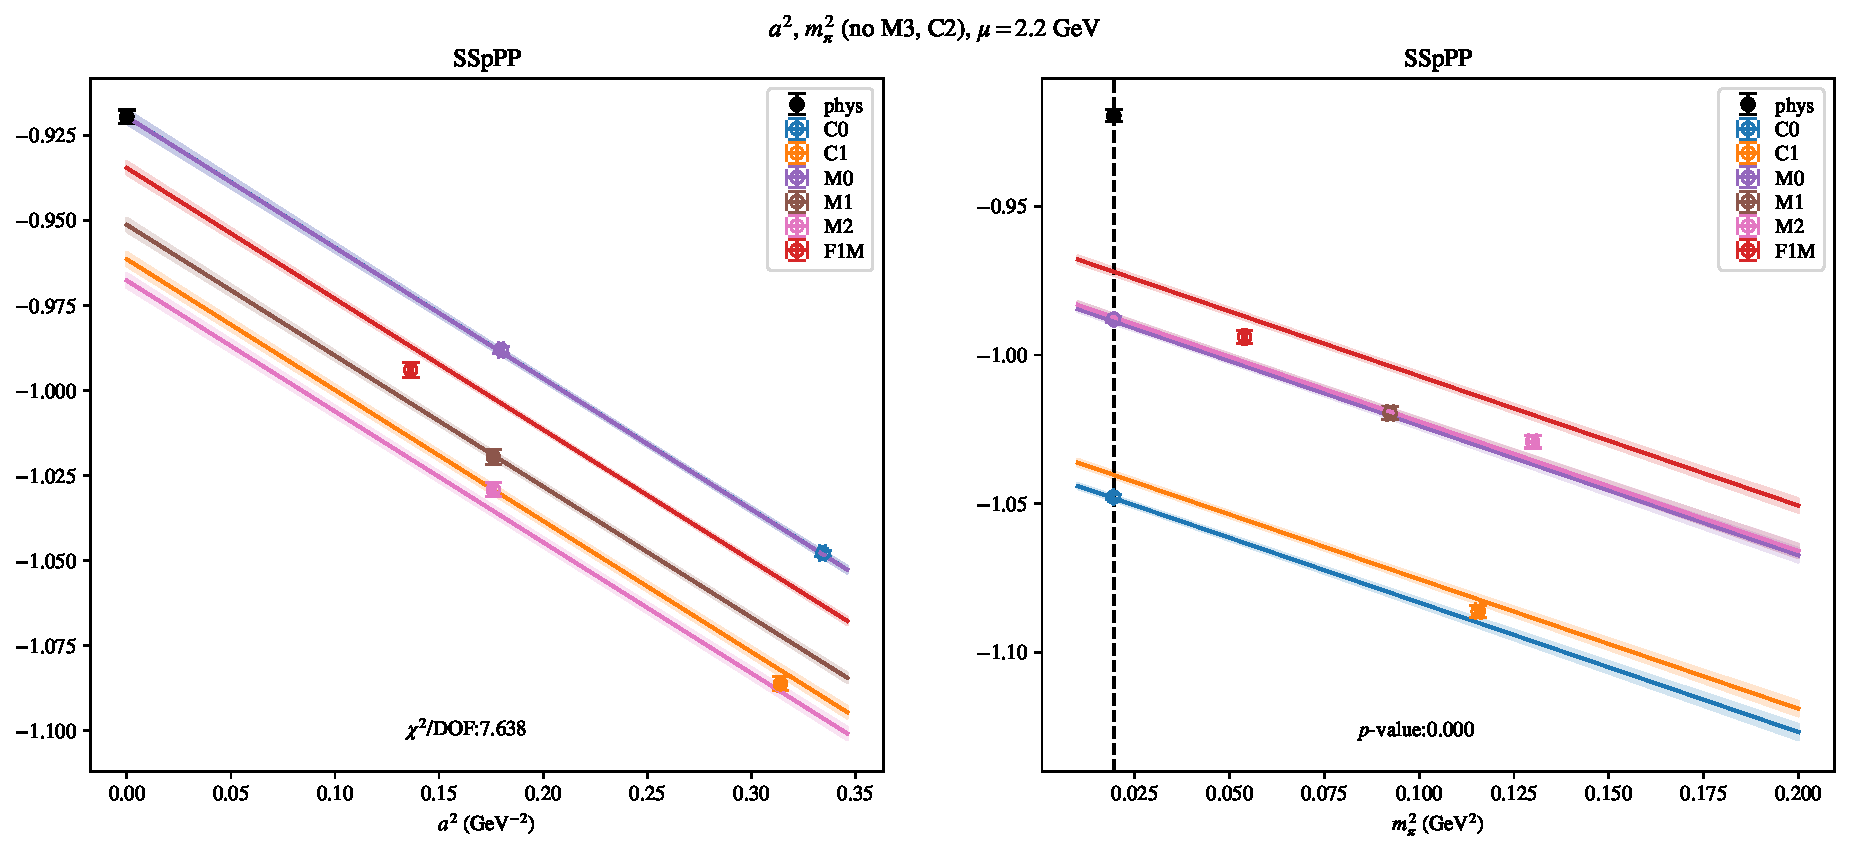
\includepdf[link, pages=-]{VVmAA/SUSY/a2m2mcut_22.pdf}
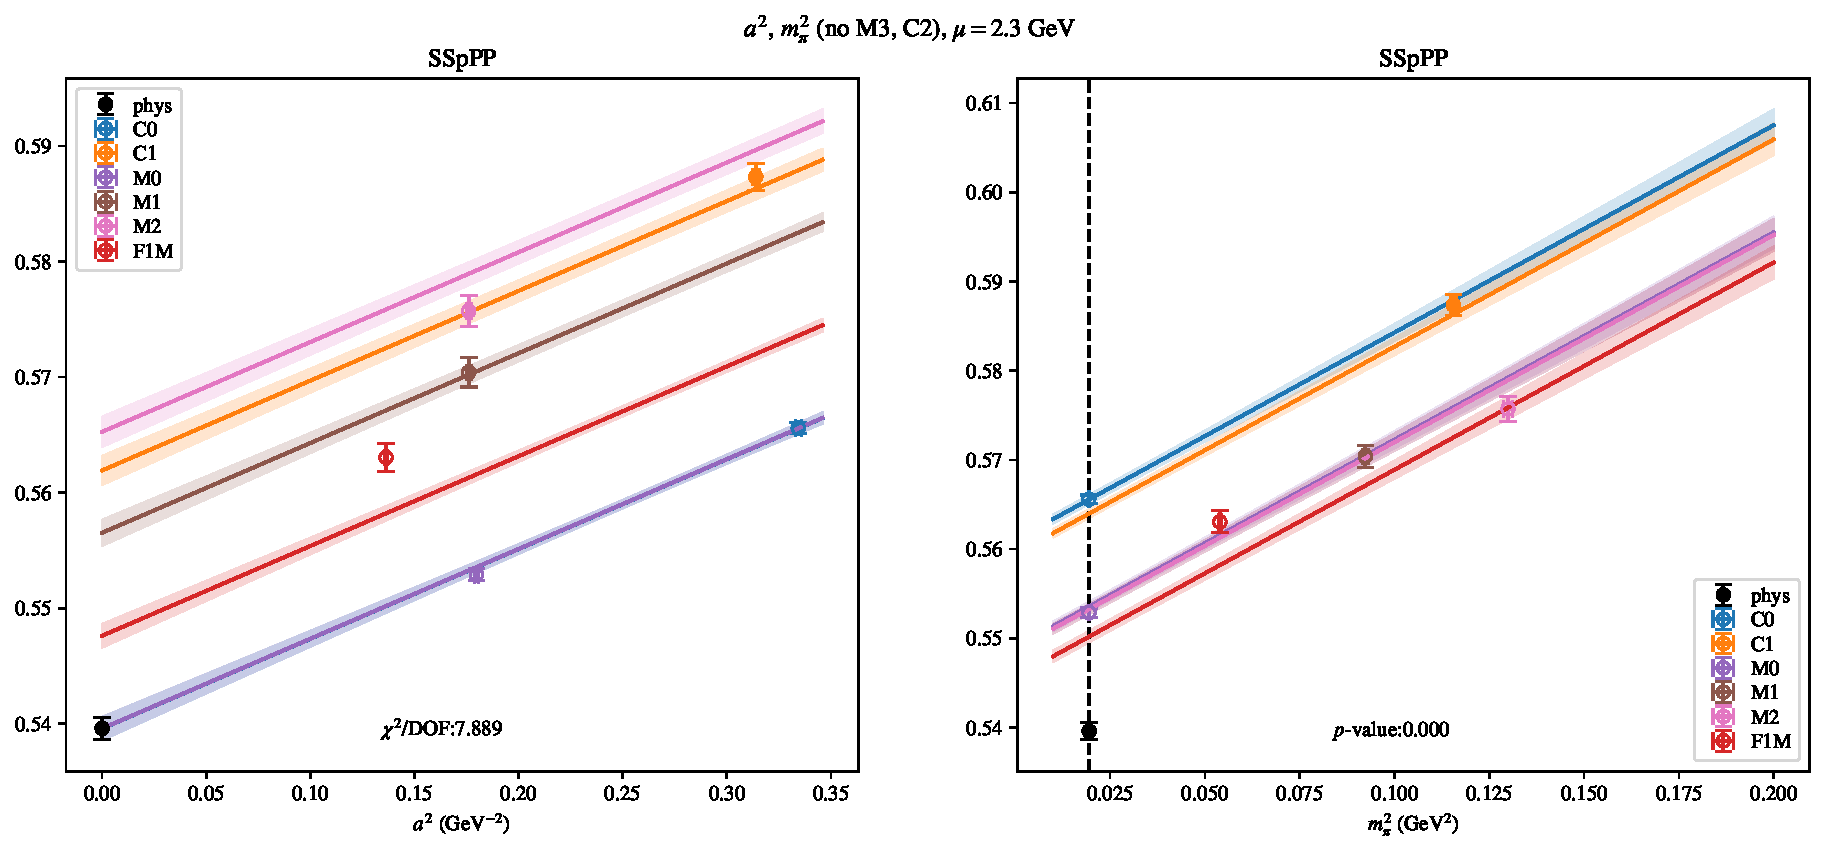
\includepdf[link, pages=-]{VVmAA/SUSY/a2m2mcut_23.pdf}
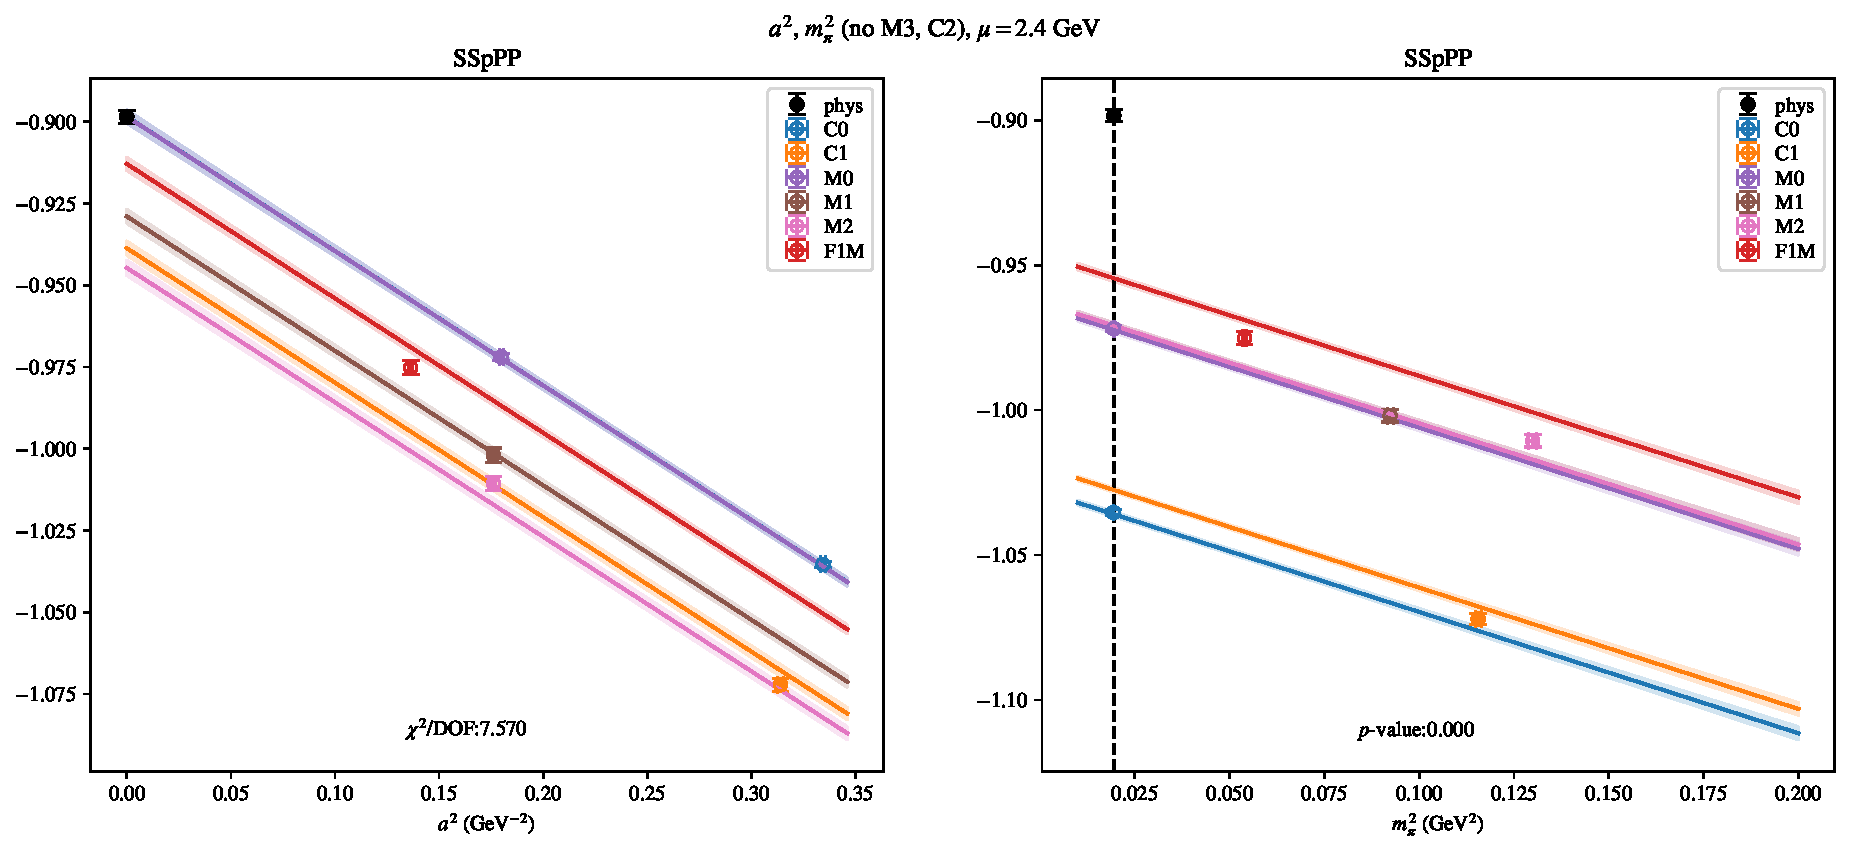
\includepdf[link, pages=-]{VVmAA/SUSY/a2m2mcut_24.pdf}
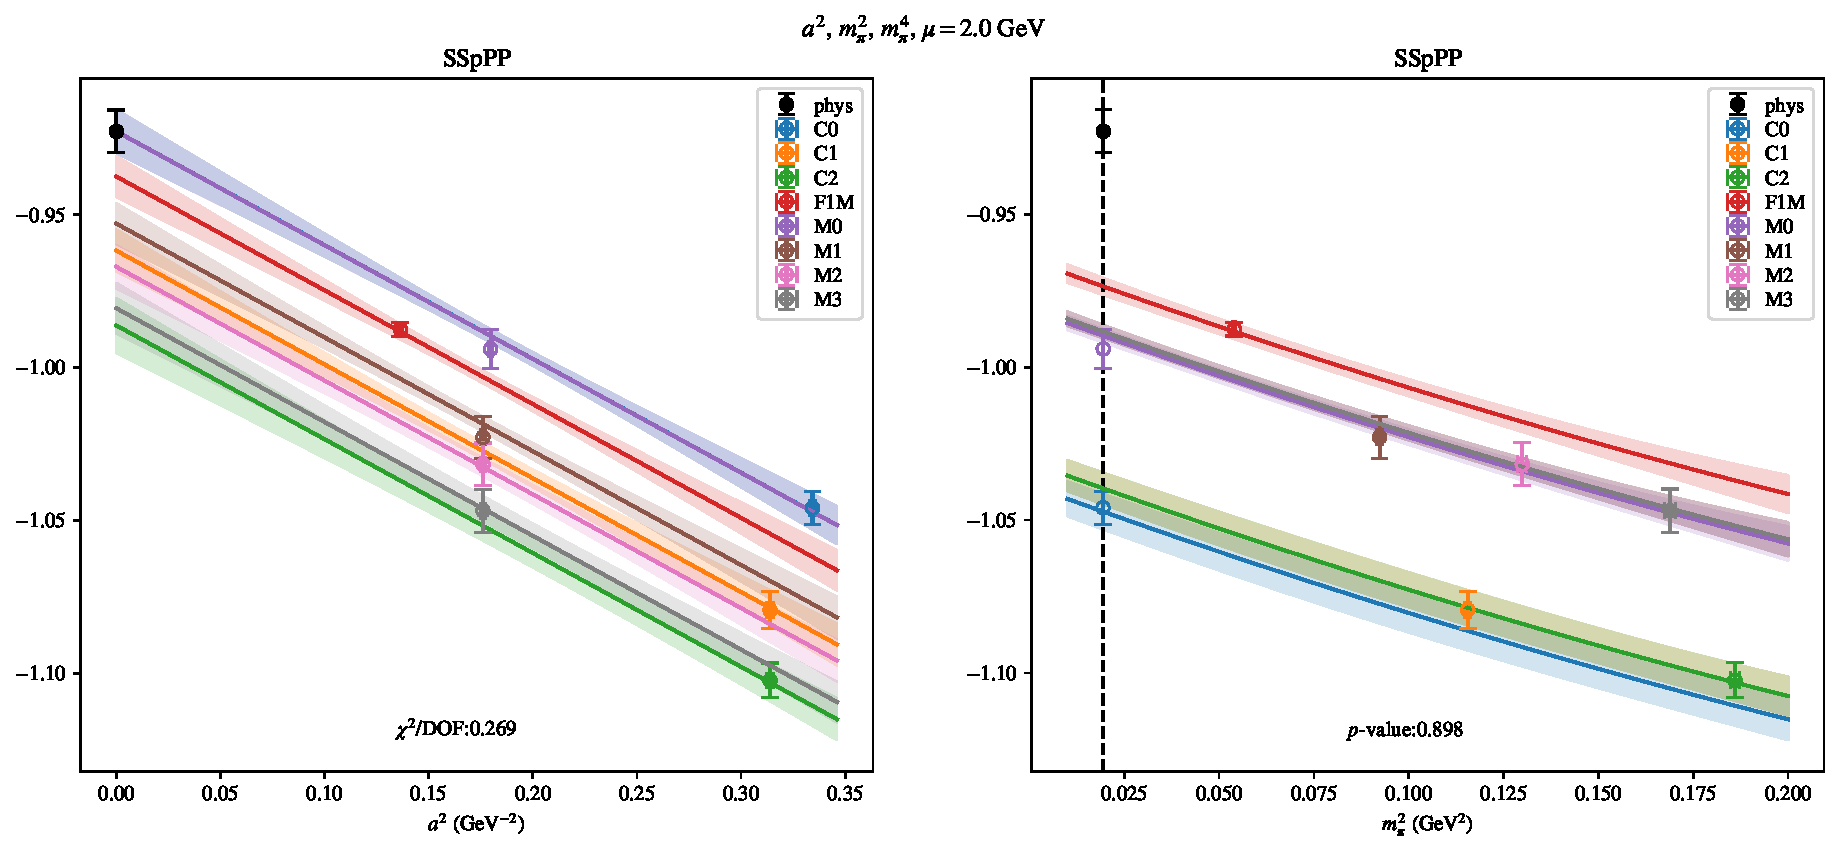
\includepdf[link, pages=-]{VVmAA/SUSY/a2m2m4_20.pdf}
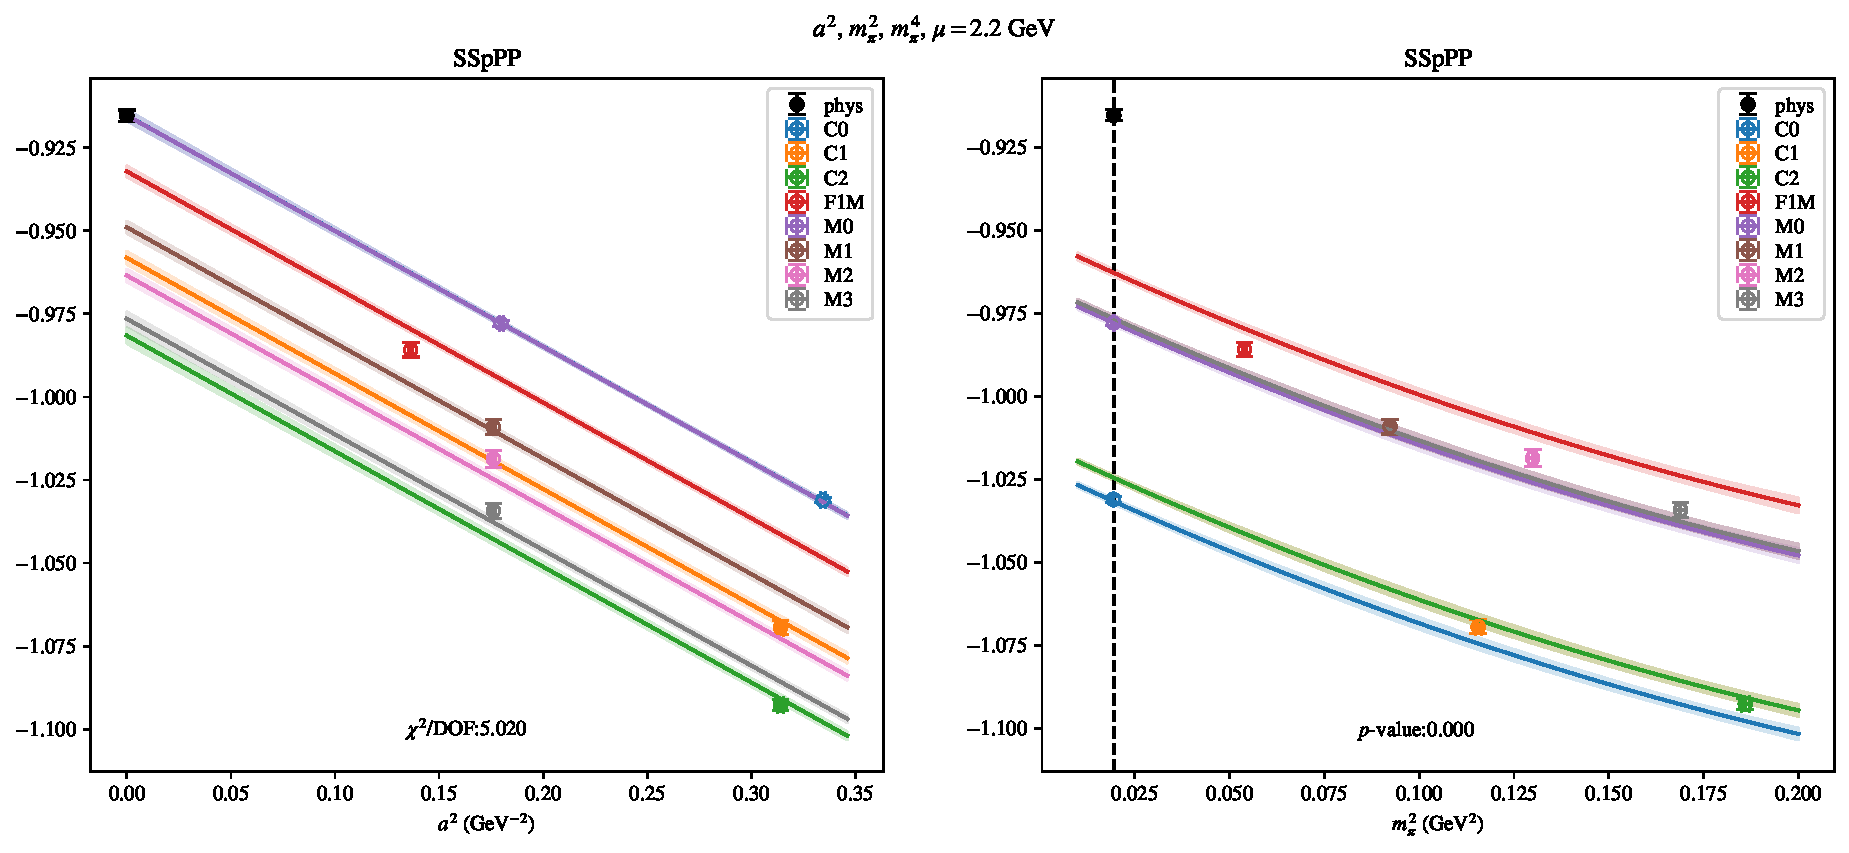
\includepdf[link, pages=-]{VVmAA/SUSY/a2m2m4_22.pdf}
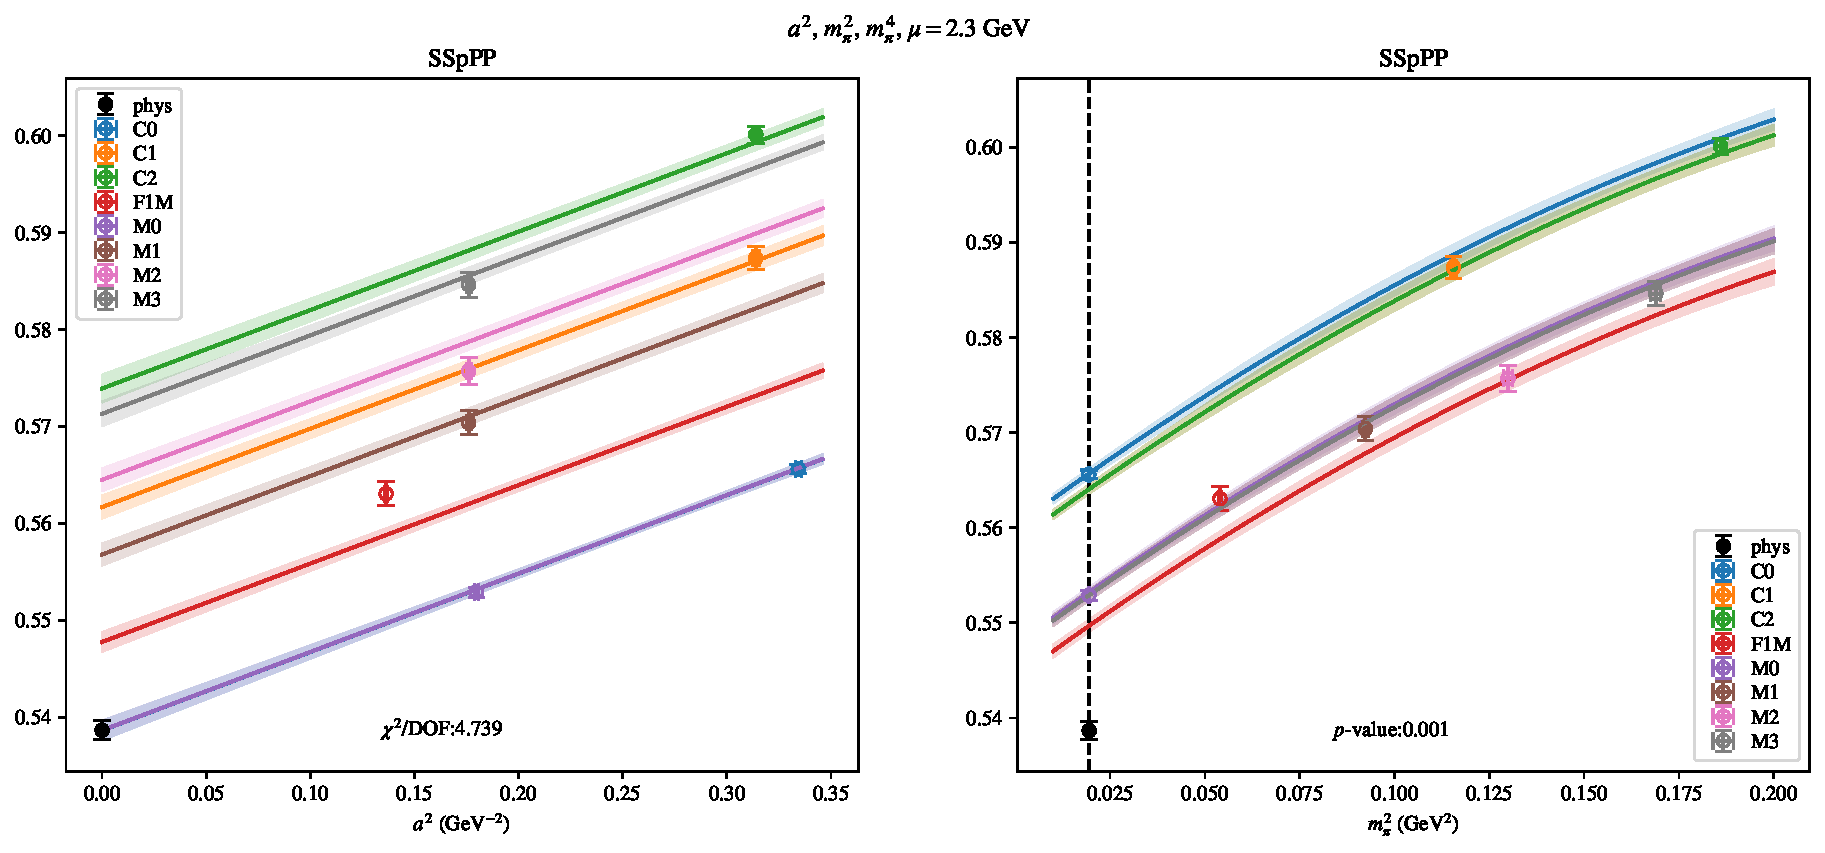
\includepdf[link, pages=-]{VVmAA/SUSY/a2m2m4_23.pdf}
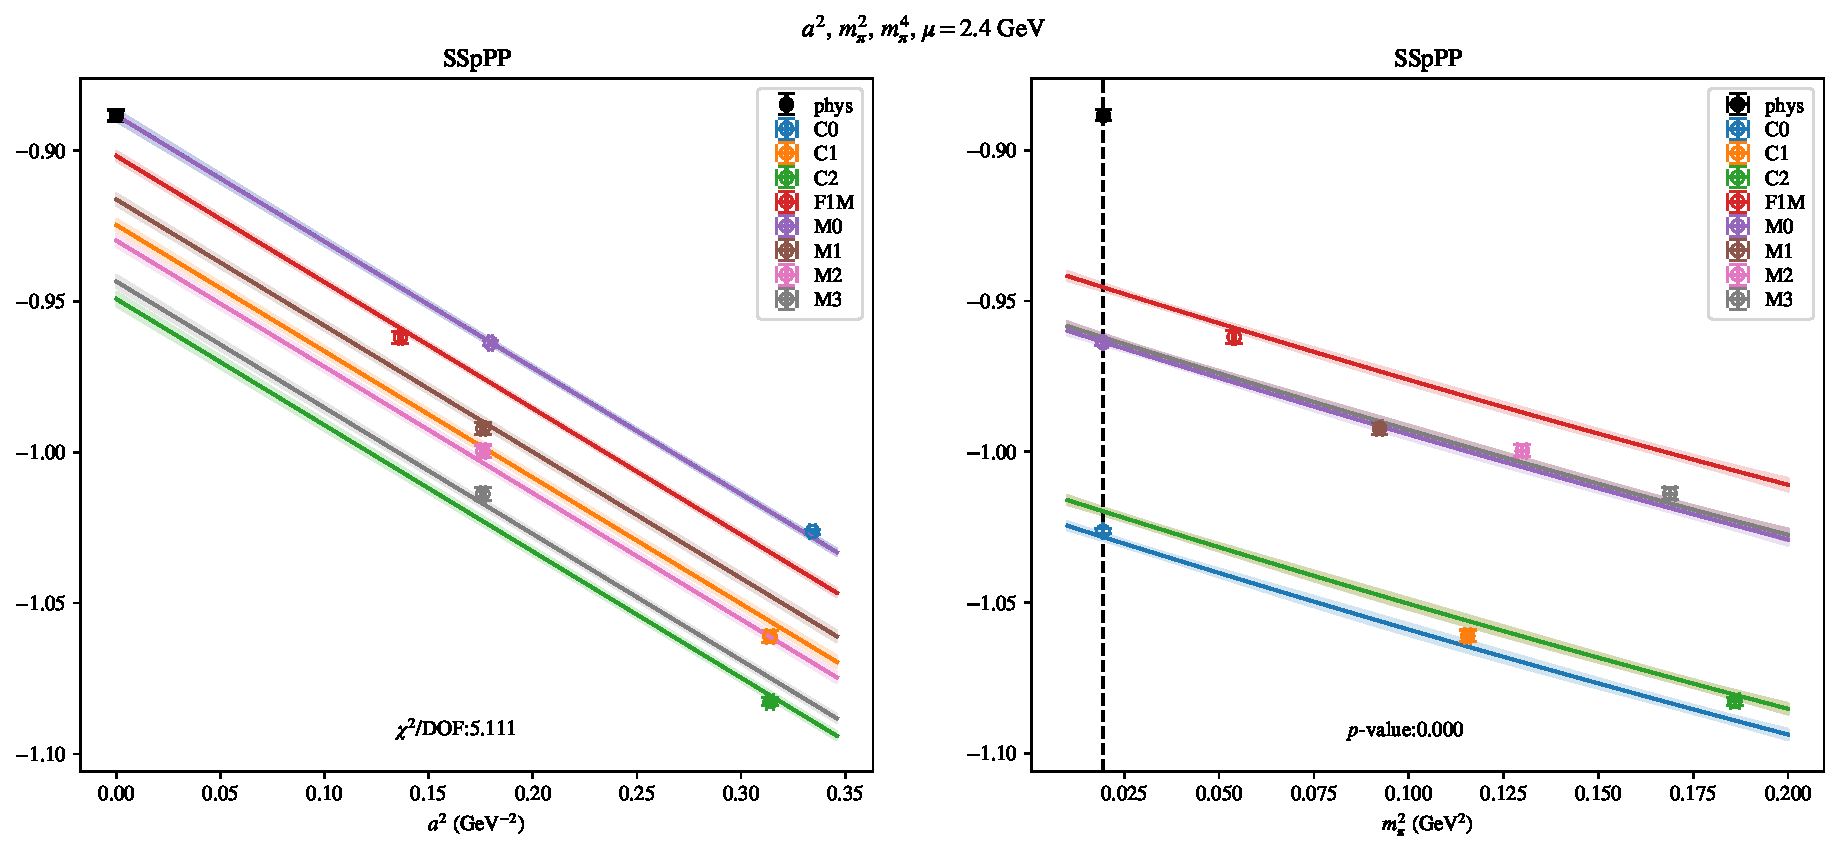
\includepdf[link, pages=-]{VVmAA/SUSY/a2m2m4_24.pdf}
\clearpage
\section{$B_3$}
\begin{table}[h!]
\begin{center}
\begin{tabular}{|c|c|c|c|c|c|}
\hline
$\mu$ (GeV) & $a^2$, $m_\pi^2$& $a^2$, $m_\pi^2$ (no C)& $a^2$, $a^4$, $m_\pi^2$& $a^2$, $m_\pi^2$ (no M3, C2)& $a^2$, $m_\pi^2$, $m_\pi^4$\\
\hline
2.0& \hyperlink{SSmPP/SUSY/a2m2_20.pdf.1}{\textbf{-0.0156(32)}: 12.183 (0.0)} & \hyperlink{SSmPP/SUSY/a2m2noC_20.pdf.1}{\textbf{-0.0215(88)}: 0.289 (0.749)} & \hyperlink{SSmPP/SUSY/a2a4m2_20.pdf.1}{\textbf{-0.029(14)}: 5.373 (0.0)} & \hyperlink{SSmPP/SUSY/a2m2mcut_20.pdf.1}{\textbf{-0.0154(40)}: 16.523 (0.0)} & \hyperlink{SSmPP/SUSY/a2m2m4_20.pdf.1}{\textbf{-0.0158(30)}: 14.807 (0.0)}\\
2.2& \hyperlink{SSmPP/SUSY/a2m2_22.pdf.1}{\textbf{-0.0031(38)}: 9.288 (0.0)} & \hyperlink{SSmPP/SUSY/a2m2noC_22.pdf.1}{\textbf{-0.0094(99)}: 0.063 (0.939)} & \hyperlink{SSmPP/SUSY/a2a4m2_22.pdf.1}{\textbf{-0.018(13)}: 2.802 (0.024)} & \hyperlink{SSmPP/SUSY/a2m2mcut_22.pdf.1}{\textbf{-0.0030(44)}: 13.108 (0.0)} & \hyperlink{SSmPP/SUSY/a2m2m4_22.pdf.1}{\textbf{-0.0033(38)}: 11.173 (0.0)}\\
2.3& \hyperlink{SSmPP/SUSY/a2m2_23.pdf.1}{\textbf{0.00188(38)}: 10.583 (0.0)} & \hyperlink{SSmPP/SUSY/a2m2noC_23.pdf.1}{\textbf{-0.0044(89)}: 0.102 (0.903)} & \hyperlink{SSmPP/SUSY/a2a4m2_23.pdf.1}{\textbf{-0.012(12)}: 3.204 (0.012)} & \hyperlink{SSmPP/SUSY/a2m2mcut_23.pdf.1}{\textbf{0.00211(41)}: 15.164 (0.0)} & \hyperlink{SSmPP/SUSY/a2m2m4_23.pdf.1}{\textbf{0.00182(36)}: 13.193 (0.0)}\\
2.4& \hyperlink{SSmPP/SUSY/a2m2_24.pdf.1}{\textbf{0.00572(36)}: 8.812 (0.0)} & \hyperlink{SSmPP/SUSY/a2m2noC_24.pdf.1}{\textbf{0.00072(83)}: 0.252 (0.777)} & \hyperlink{SSmPP/SUSY/a2a4m2_24.pdf.1}{\textbf{-0.006(12)}: 3.786 (0.004)} & \hyperlink{SSmPP/SUSY/a2m2mcut_24.pdf.1}{\textbf{0.00595(39)}: 11.863 (0.0)} & \hyperlink{SSmPP/SUSY/a2m2m4_24.pdf.1}{\textbf{0.00559(35)}: 10.86 (0.0)}\\
\hline
\end{tabular}
\caption{Physical point value from chiral and continuum extrapolation at renormalisation scale $\mu$. Entries are \textbf{value(error)}: $\chi^2/\text{DOF}$ ($p$-value).}
\end{center}
\end{table}
\begin{table}[h!]
\begin{center}
\begin{tabular}{|c c|c|c|c|c|c|}
\hline
$\mu$ (GeV) &  & $a^2$, $m_\pi^2$& $a^2$, $m_\pi^2$ (no C)& $a^2$, $a^4$, $m_\pi^2$& $a^2$, $m_\pi^2$ (no M3, C2)& $a^2$, $m_\pi^2$, $m_\pi^4$\\
\hline
\multirow{2}{0.5in}{2.0} & $\alpha$ & -12.(26)& -10.(27)& -10.(15)& -12.(31)& -12.(24)\\
 & $\beta$ & -0.0086(72)& 0.0011(11)& -0.0016(52)& -0.012(14)& -0.016(41)\\
\hline
\multirow{2}{0.5in}{2.2} & $\alpha$ & -57(79)& -23(23)& -17.(81)& -59(98)& -54(67)\\
 & $\beta$ & -0.067(97)& -0.008(17)& -0.0075(99)& -0.08(14)& -0.10(21)\\
\hline
\multirow{2}{0.5in}{2.3} & $\alpha$ & 96(22)& -4(13)& -24(18)& 85(20)& 99(23)\\
 & $\beta$ & 0.136(29)& -0.024(81)& -0.014(21)& 0.133(29)& 0.161(50)\\
\hline
\multirow{2}{0.5in}{2.4} & $\alpha$ & 31.(20)& 295.62& -4(12)& 30.(20)& 32.(20)\\
 & $\beta$ & 0.0491(33)& 0.192& -0.03(12)& 0.0522(47)& 0.064(12)\\
\hline
\end{tabular}
\caption{Fit values of coefficients in $B = B_{phys} + \mathbf{\alpha} a^2 + \mathbf{\beta}\left(\frac{m_\pi^2}{f_\pi^2}-\frac{m_{\pi,PDG}^2}{f_\pi^2}\right) + \ldots$.}
\end{center}
\end{table}
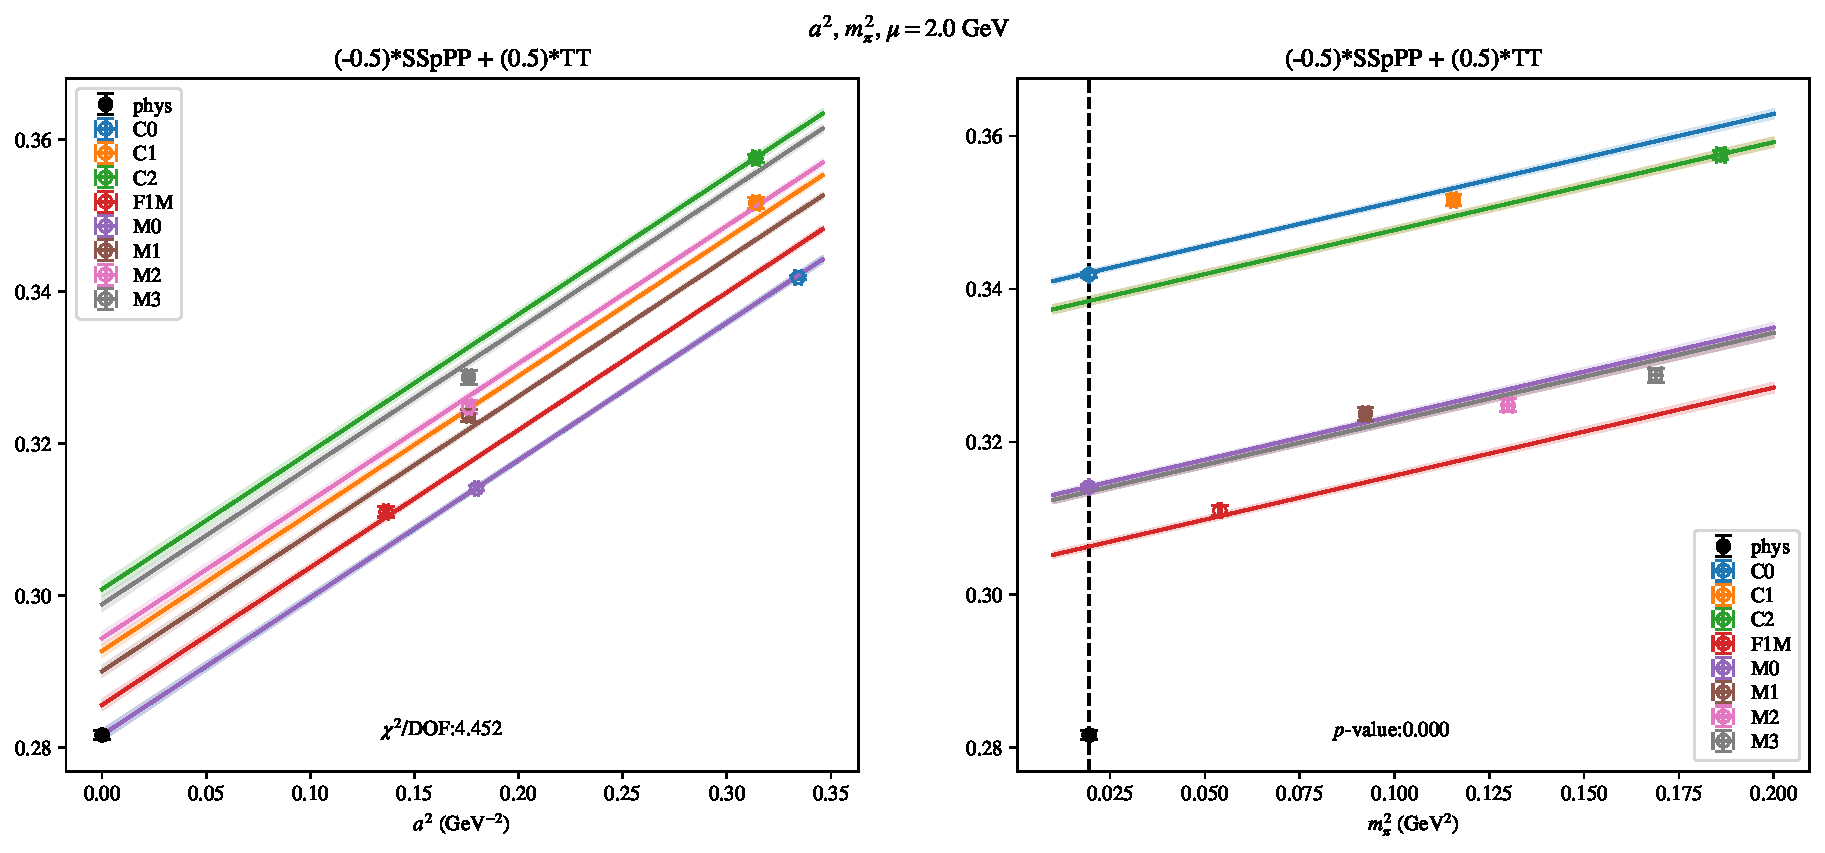
\includepdf[link, pages=-]{SSmPP/SUSY/a2m2_20.pdf}
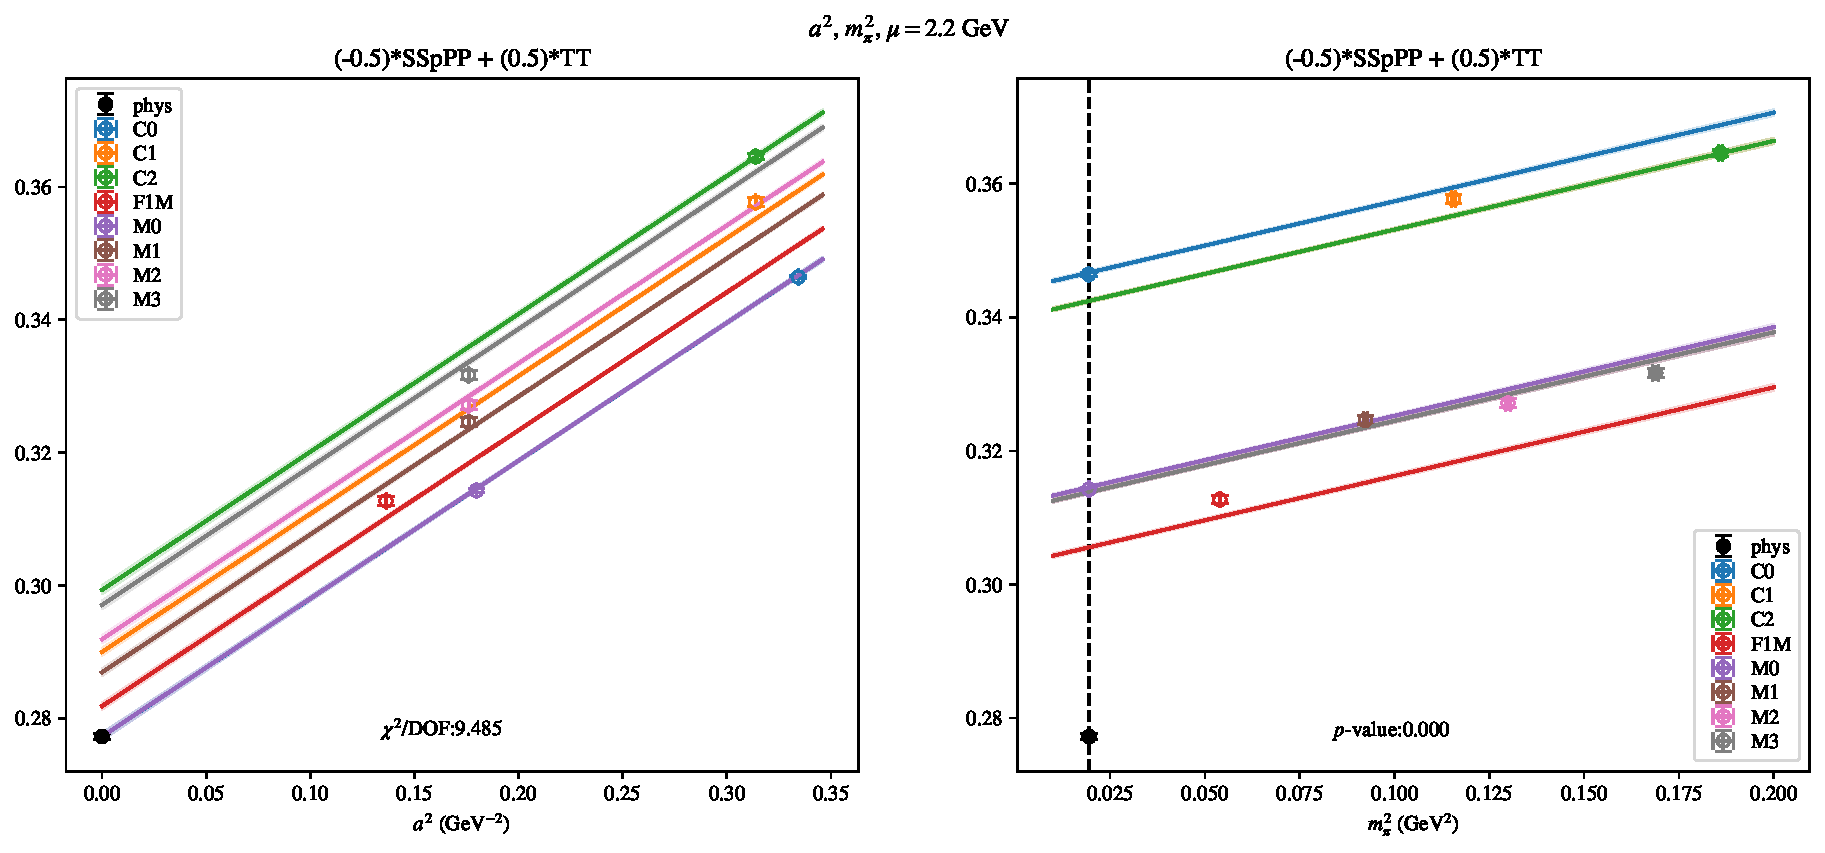
\includepdf[link, pages=-]{SSmPP/SUSY/a2m2_22.pdf}
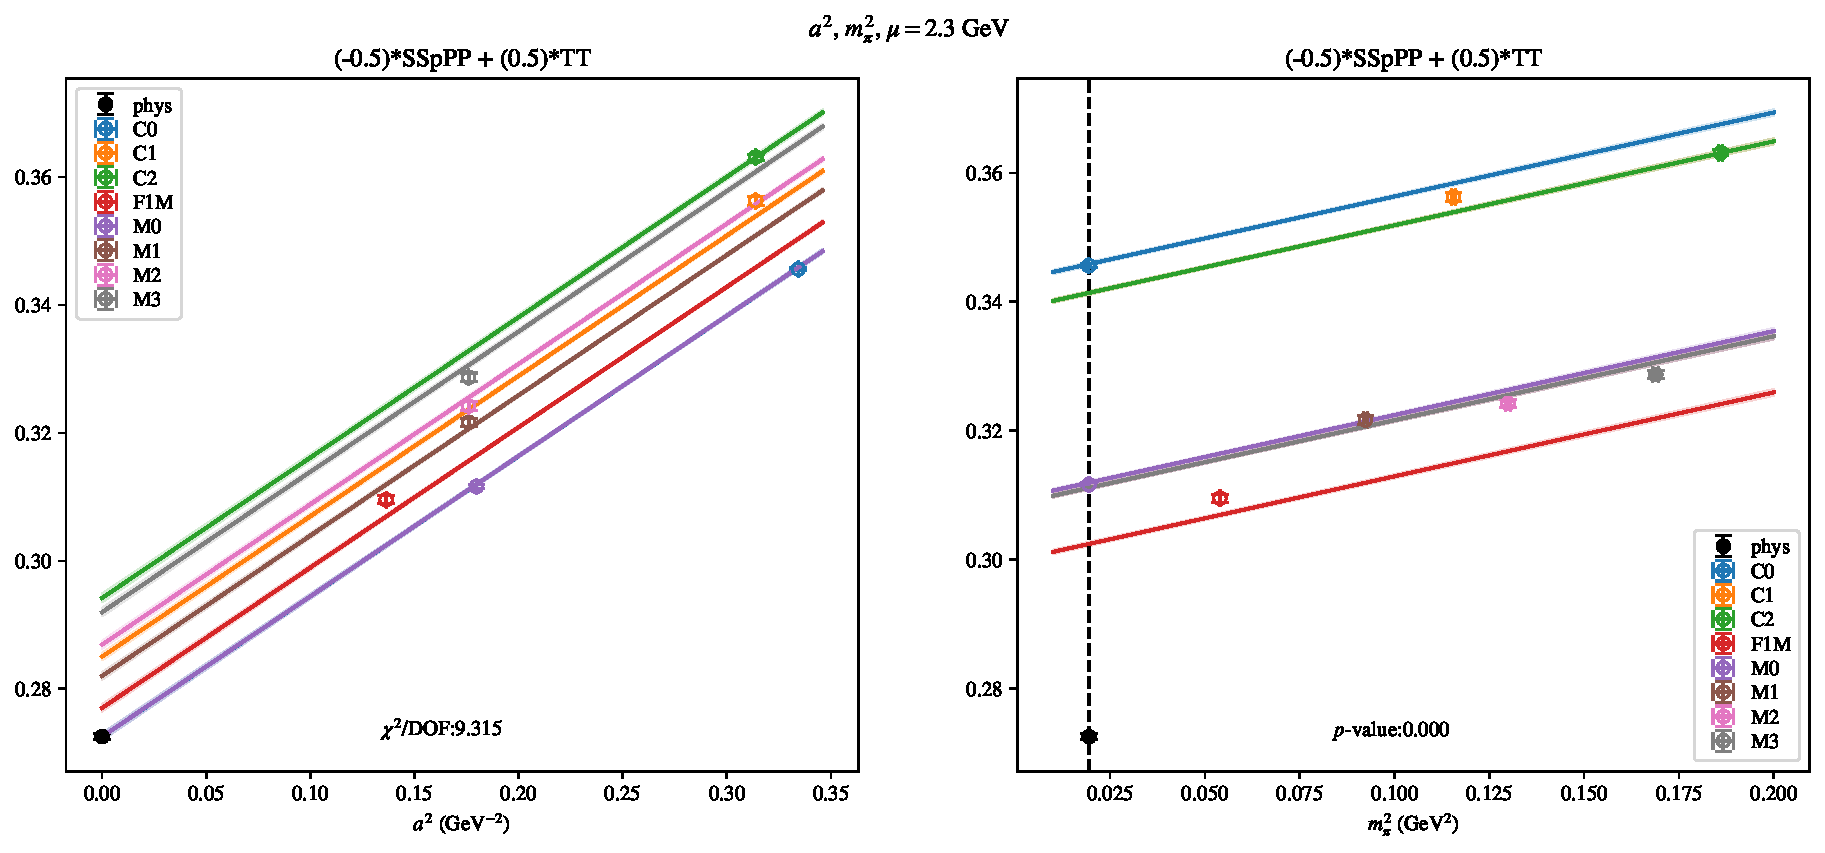
\includepdf[link, pages=-]{SSmPP/SUSY/a2m2_23.pdf}
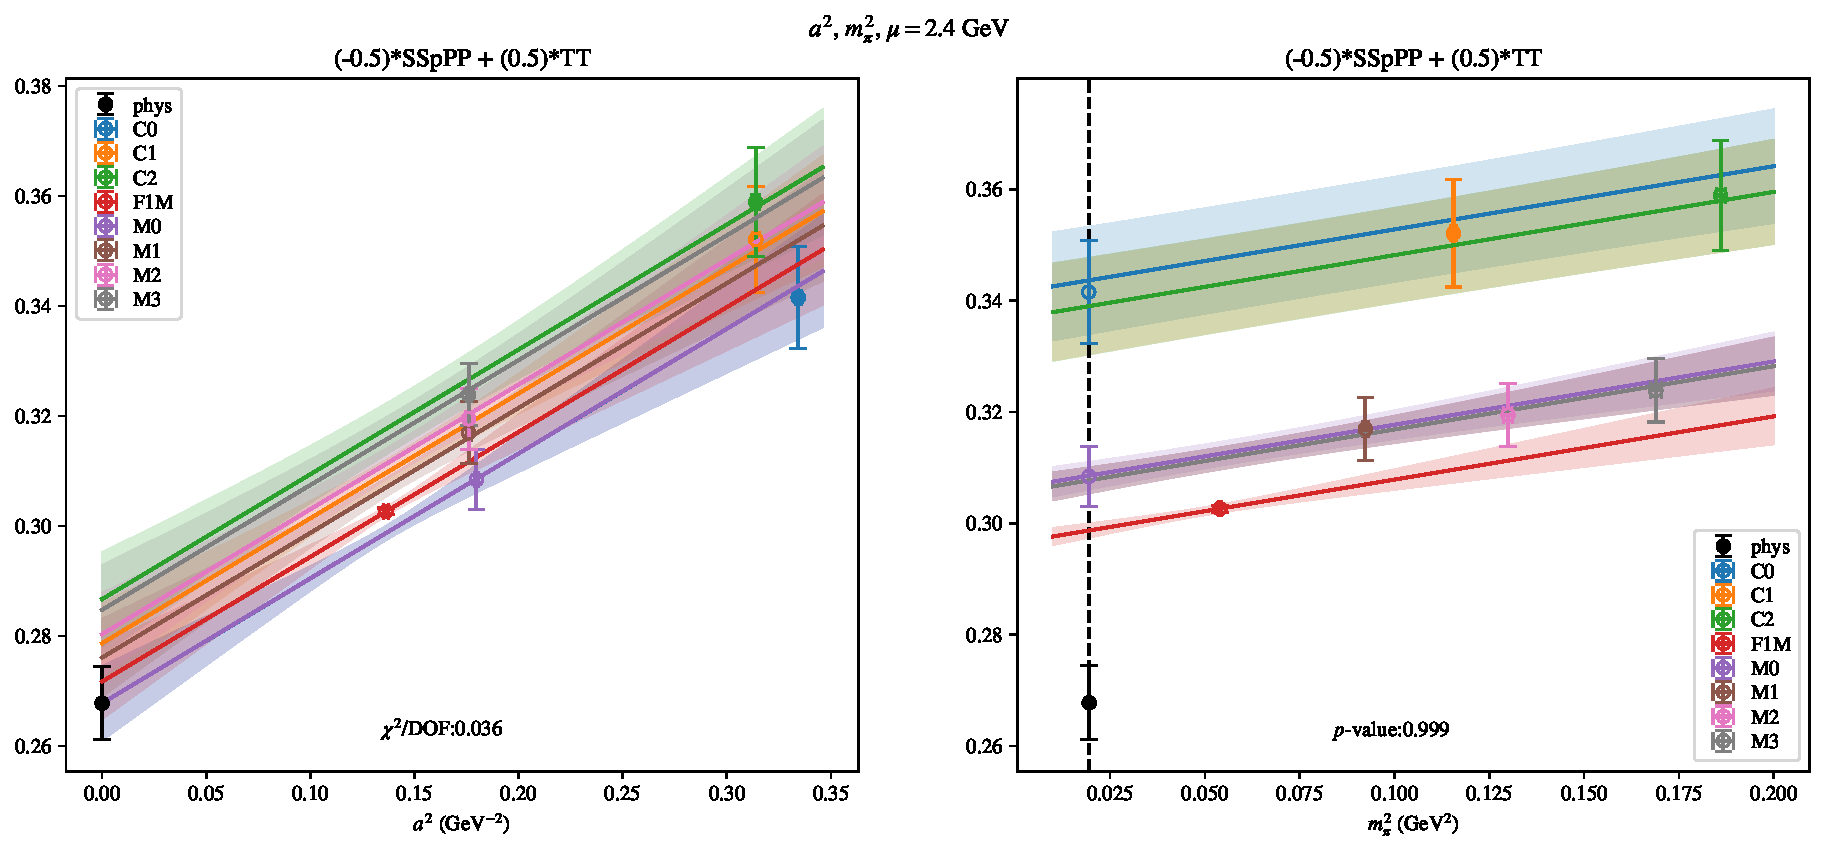
\includepdf[link, pages=-]{SSmPP/SUSY/a2m2_24.pdf}
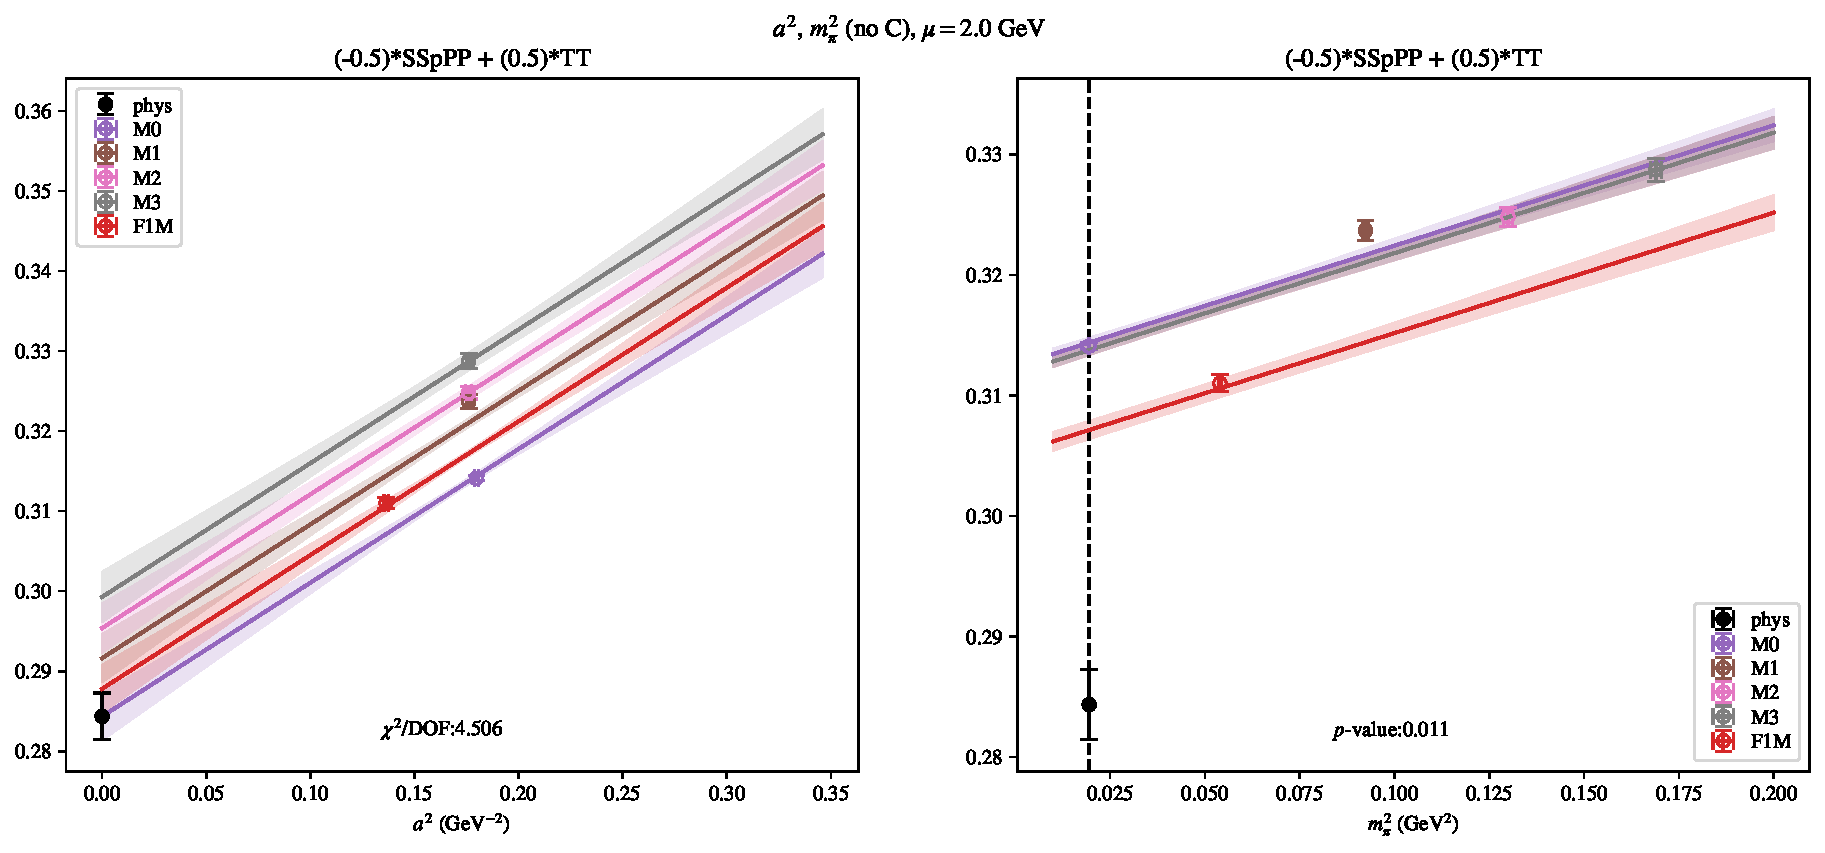
\includepdf[link, pages=-]{SSmPP/SUSY/a2m2noC_20.pdf}
\includepdf[link, pages=-]{SSmPP/SUSY/a2m2noC_22.pdf}
\includepdf[link, pages=-]{SSmPP/SUSY/a2m2noC_23.pdf}
\includepdf[link, pages=-]{SSmPP/SUSY/a2m2noC_24.pdf}
\includepdf[link, pages=-]{SSmPP/SUSY/a2a4m2_20.pdf}
\includepdf[link, pages=-]{SSmPP/SUSY/a2a4m2_22.pdf}
\includepdf[link, pages=-]{SSmPP/SUSY/a2a4m2_23.pdf}
\includepdf[link, pages=-]{SSmPP/SUSY/a2a4m2_24.pdf}
\includepdf[link, pages=-]{SSmPP/SUSY/a2m2mcut_20.pdf}
\includepdf[link, pages=-]{SSmPP/SUSY/a2m2mcut_22.pdf}
\includepdf[link, pages=-]{SSmPP/SUSY/a2m2mcut_23.pdf}
\includepdf[link, pages=-]{SSmPP/SUSY/a2m2mcut_24.pdf}
\includepdf[link, pages=-]{SSmPP/SUSY/a2m2m4_20.pdf}
\includepdf[link, pages=-]{SSmPP/SUSY/a2m2m4_22.pdf}
\includepdf[link, pages=-]{SSmPP/SUSY/a2m2m4_23.pdf}
\includepdf[link, pages=-]{SSmPP/SUSY/a2m2m4_24.pdf}
\clearpage
\section{$B_4$}
\begin{table}[h!]
\begin{center}
\begin{tabular}{|c|c|c|c|c|c|}
\hline
$\mu$ (GeV) & $a^2$, $m_\pi^2$& $a^2$, $m_\pi^2$ (no C)& $a^2$, $a^4$, $m_\pi^2$& $a^2$, $m_\pi^2$ (no M3, C2)& $a^2$, $m_\pi^2$, $m_\pi^4$\\
\hline
2.0& \hyperlink{SSpPP/SUSY/a2m2_20.pdf.1}{\textbf{0.9556(13)}: 5.291 (0.0)} & \hyperlink{SSpPP/SUSY/a2m2noC_20.pdf.1}{\textbf{0.9258(69)}: 2.847 (0.058)} & \hyperlink{SSpPP/SUSY/a2a4m2_20.pdf.1}{\textbf{0.906(10)}: 1.648 (0.159)} & \hyperlink{SSpPP/SUSY/a2m2mcut_20.pdf.1}{\textbf{0.9559(15)}: 7.328 (0.0)} & \hyperlink{SSpPP/SUSY/a2m2m4_20.pdf.1}{\textbf{0.9575(15)}: 4.551 (0.001)}\\
2.2& \hyperlink{SSpPP/SUSY/a2m2_22.pdf.1}{\textbf{0.9484(13)}: 5.761 (0.0)} & \hyperlink{SSpPP/SUSY/a2m2noC_22.pdf.1}{\textbf{0.9161(66)}: 1.667 (0.189)} & \hyperlink{SSpPP/SUSY/a2a4m2_22.pdf.1}{\textbf{0.894(10)}: 1.011 (0.4)} & \hyperlink{SSpPP/SUSY/a2m2mcut_22.pdf.1}{\textbf{0.9487(14)}: 8.642 (0.0)} & \hyperlink{SSpPP/SUSY/a2m2m4_22.pdf.1}{\textbf{0.9502(14)}: 5.436 (0.0)}\\
2.3& \hyperlink{SSpPP/SUSY/a2m2_23.pdf.1}{\textbf{0.9455(13)}: 6.084 (0.0)} & \hyperlink{SSpPP/SUSY/a2m2noC_23.pdf.1}{\textbf{0.9125(66)}: 1.868 (0.154)} & \hyperlink{SSpPP/SUSY/a2a4m2_23.pdf.1}{\textbf{0.890(10)}: 1.19 (0.313)} & \hyperlink{SSpPP/SUSY/a2m2mcut_23.pdf.1}{\textbf{0.9459(14)}: 9.145 (0.0)} & \hyperlink{SSpPP/SUSY/a2m2m4_23.pdf.1}{\textbf{0.9474(14)}: 5.664 (0.0)}\\
2.4& \hyperlink{SSpPP/SUSY/a2m2_24.pdf.1}{\textbf{0.9435(13)}: 6.941 (0.0)} & \hyperlink{SSpPP/SUSY/a2m2noC_24.pdf.1}{\textbf{0.9087(66)}: 2.162 (0.115)} & \hyperlink{SSpPP/SUSY/a2a4m2_24.pdf.1}{\textbf{0.885(10)}: 1.323 (0.258)} & \hyperlink{SSpPP/SUSY/a2m2mcut_24.pdf.1}{\textbf{0.9440(14)}: 10.457 (0.0)} & \hyperlink{SSpPP/SUSY/a2m2m4_24.pdf.1}{\textbf{0.9456(14)}: 6.402 (0.0)}\\
\hline
\end{tabular}
\caption{Physical point value from chiral and continuum extrapolation at renormalisation scale $\mu$. Entries are \textbf{value(error)}: $\chi^2/\text{DOF}$ ($p$-value).}
\end{center}
\end{table}
\begin{table}[h!]
\begin{center}
\begin{tabular}{|c c|c|c|c|c|c|}
\hline
$\mu$ (GeV) &  & $a^2$, $m_\pi^2$& $a^2$, $m_\pi^2$ (no C)& $a^2$, $a^4$, $m_\pi^2$& $a^2$, $m_\pi^2$ (no M3, C2)& $a^2$, $m_\pi^2$, $m_\pi^4$\\
\hline
\multirow{2}{0.5in}{2.0} & $\alpha$ & 0.1383(55)& 0.329(44)& 0.62(11)& 0.1375(61)& 0.1314(60)\\
 & $\beta$ & 0.00024(13)& 0.00023(23)& 0.0& -0.0& -0.0016(64)\\
\hline
\multirow{2}{0.5in}{2.2} & $\alpha$ & 0.1534(56)& 0.364(44)& 0.70(11)& 0.1526(60)& 0.1470(60)\\
 & $\beta$ & -0.0& -0.0& -0.0002(13)& -0.0003(23)& -0.0017(67)\\
\hline
\multirow{2}{0.5in}{2.3} & $\alpha$ & 0.1618(56)& 0.379(44)& 0.72(11)& 0.1607(60)& 0.1549(60)\\
 & $\beta$ & -0.0& -0.0001(21)& -0.0003(13)& -0.0003(22)& -0.0018(65)\\
\hline
\multirow{2}{0.5in}{2.4} & $\alpha$ & 0.1685(56)& 0.399(44)& 0.76(11)& 0.1671(60)& 0.1610(60)\\
 & $\beta$ & -0.0001(11)& -0.0002(20)& -0.0003(12)& -0.0004(21)& -0.0020(63)\\
\hline
\end{tabular}
\caption{Fit values of coefficients in $B = B_{phys} + \mathbf{\alpha} a^2 + \mathbf{\beta}\left(\frac{m_\pi^2}{f_\pi^2}-\frac{m_{\pi,PDG}^2}{f_\pi^2}\right) + \ldots$.}
\end{center}
\end{table}
\includepdf[link, pages=-]{SSpPP/SUSY/a2m2_20.pdf}
\includepdf[link, pages=-]{SSpPP/SUSY/a2m2_22.pdf}
\includepdf[link, pages=-]{SSpPP/SUSY/a2m2_23.pdf}
\includepdf[link, pages=-]{SSpPP/SUSY/a2m2_24.pdf}
\includepdf[link, pages=-]{SSpPP/SUSY/a2m2noC_20.pdf}
\includepdf[link, pages=-]{SSpPP/SUSY/a2m2noC_22.pdf}
\includepdf[link, pages=-]{SSpPP/SUSY/a2m2noC_23.pdf}
\includepdf[link, pages=-]{SSpPP/SUSY/a2m2noC_24.pdf}
\includepdf[link, pages=-]{SSpPP/SUSY/a2a4m2_20.pdf}
\includepdf[link, pages=-]{SSpPP/SUSY/a2a4m2_22.pdf}
\includepdf[link, pages=-]{SSpPP/SUSY/a2a4m2_23.pdf}
\includepdf[link, pages=-]{SSpPP/SUSY/a2a4m2_24.pdf}
\includepdf[link, pages=-]{SSpPP/SUSY/a2m2mcut_20.pdf}
\includepdf[link, pages=-]{SSpPP/SUSY/a2m2mcut_22.pdf}
\includepdf[link, pages=-]{SSpPP/SUSY/a2m2mcut_23.pdf}
\includepdf[link, pages=-]{SSpPP/SUSY/a2m2mcut_24.pdf}
\includepdf[link, pages=-]{SSpPP/SUSY/a2m2m4_20.pdf}
\includepdf[link, pages=-]{SSpPP/SUSY/a2m2m4_22.pdf}
\includepdf[link, pages=-]{SSpPP/SUSY/a2m2m4_23.pdf}
\includepdf[link, pages=-]{SSpPP/SUSY/a2m2m4_24.pdf}
\clearpage
\section{$B_5$}
\begin{table}[h!]
\begin{center}
\begin{tabular}{|c|c|c|c|c|c|}
\hline
$\mu$ (GeV) & $a^2$, $m_\pi^2$& $a^2$, $m_\pi^2$ (no C)& $a^2$, $a^4$, $m_\pi^2$& $a^2$, $m_\pi^2$ (no M3, C2)& $a^2$, $m_\pi^2$, $m_\pi^4$\\
\hline
2.0& \hyperlink{TT/SUSY/a2m2_20.pdf.1}{\textbf{-1.191(45)}: 2.148 (0.057)} & \hyperlink{TT/SUSY/a2m2noC_20.pdf.1}{\textbf{-1.234(87)}: 0.127 (0.881)} & \hyperlink{TT/SUSY/a2a4m2_20.pdf.1}{\textbf{-1.27(13)}: 0.162 (0.958)} & \hyperlink{TT/SUSY/a2m2mcut_20.pdf.1}{\textbf{-1.190(42)}: 3.396 (0.017)} & \hyperlink{TT/SUSY/a2m2m4_20.pdf.1}{\textbf{-1.190(42)}: 2.598 (0.034)}\\
2.2& \hyperlink{TT/SUSY/a2m2_22.pdf.1}{\textbf{-1.080(44)}: 2.039 (0.07)} & \hyperlink{TT/SUSY/a2m2noC_22.pdf.1}{\textbf{-1.127(90)}: 0.026 (0.975)} & \hyperlink{TT/SUSY/a2a4m2_22.pdf.1}{\textbf{-1.15(13)}: 0.163 (0.957)} & \hyperlink{TT/SUSY/a2m2mcut_22.pdf.1}{\textbf{-1.079(41)}: 3.389 (0.017)} & \hyperlink{TT/SUSY/a2m2m4_22.pdf.1}{\textbf{-1.078(41)}: 2.437 (0.045)}\\
2.3& \hyperlink{TT/SUSY/a2m2_23.pdf.1}{\textbf{-1.032(39)}: 2.88 (0.013)} & \hyperlink{TT/SUSY/a2m2noC_23.pdf.1}{\textbf{-1.082(83)}: 0.049 (0.952)} & \hyperlink{TT/SUSY/a2a4m2_23.pdf.1}{\textbf{-1.11(12)}: 0.147 (0.964)} & \hyperlink{TT/SUSY/a2m2mcut_23.pdf.1}{\textbf{-1.032(36)}: 4.762 (0.003)} & \hyperlink{TT/SUSY/a2m2m4_23.pdf.1}{\textbf{-1.031(36)}: 3.416 (0.008)}\\
2.4& \hyperlink{TT/SUSY/a2m2_24.pdf.1}{\textbf{-0.994(37)}: 2.333 (0.04)} & \hyperlink{TT/SUSY/a2m2noC_24.pdf.1}{\textbf{-1.035(77)}: 0.235 (0.79)} & \hyperlink{TT/SUSY/a2a4m2_24.pdf.1}{\textbf{-1.06(11)}: 0.359 (0.838)} & \hyperlink{TT/SUSY/a2m2mcut_24.pdf.1}{\textbf{-0.994(35)}: 3.883 (0.009)} & \hyperlink{TT/SUSY/a2m2m4_24.pdf.1}{\textbf{-0.993(35)}: 2.86 (0.022)}\\
\hline
\end{tabular}
\caption{Physical point value from chiral and continuum extrapolation at renormalisation scale $\mu$. Entries are \textbf{value(error)}: $\chi^2/\text{DOF}$ ($p$-value).}
\end{center}
\end{table}
\begin{table}[h!]
\begin{center}
\begin{tabular}{|c c|c|c|c|c|c|}
\hline
$\mu$ (GeV) &  & $a^2$, $m_\pi^2$& $a^2$, $m_\pi^2$ (no C)& $a^2$, $a^4$, $m_\pi^2$& $a^2$, $m_\pi^2$ (no M3, C2)& $a^2$, $m_\pi^2$, $m_\pi^4$\\
\hline
\multirow{2}{0.5in}{2.0} & $\alpha$ & -0.692(41)& -0.88(31)& -1.25(79)& -0.690(42)& -0.690(43)\\
 & $\beta$ & 0.00103(14)& 0.00152(24)& 0.00131(13)& 0.00102(25)& 0.00168(64)\\
\hline
\multirow{2}{0.5in}{2.2} & $\alpha$ & -0.639(49)& -0.86(32)& -1.21(81)& -0.638(48)& -0.637(48)\\
 & $\beta$ & 0.00083(12)& 0.00102(22)& 0.00111(12)& 0.00087(24)& 0.00152(67)\\
\hline
\multirow{2}{0.5in}{2.3} & $\alpha$ & -0.607(50)& -0.85(32)& -1.25(79)& -0.606(47)& -0.605(48)\\
 & $\beta$ & 0.00073(14)& 0.00099(24)& 0.00105(13)& 0.00079(27)& 0.00160(70)\\
\hline
\multirow{2}{0.5in}{2.4} & $\alpha$ & -0.584(52)& -0.80(32)& -1.13(81)& -0.584(51)& -0.582(52)\\
 & $\beta$ & 0.00079(11)& 0.00094(19)& 0.00108(11)& 0.00078(22)& 0.00124(64)\\
\hline
\end{tabular}
\caption{Fit values of coefficients in $B = B_{phys} + \mathbf{\alpha} a^2 + \mathbf{\beta}\left(\frac{m_\pi^2}{f_\pi^2}-\frac{m_{\pi,PDG}^2}{f_\pi^2}\right) + \ldots$.}
\end{center}
\end{table}
\includepdf[link, pages=-]{TT/SUSY/a2m2_20.pdf}
\includepdf[link, pages=-]{TT/SUSY/a2m2_22.pdf}
\includepdf[link, pages=-]{TT/SUSY/a2m2_23.pdf}
\includepdf[link, pages=-]{TT/SUSY/a2m2_24.pdf}
\includepdf[link, pages=-]{TT/SUSY/a2m2noC_20.pdf}
\includepdf[link, pages=-]{TT/SUSY/a2m2noC_22.pdf}
\includepdf[link, pages=-]{TT/SUSY/a2m2noC_23.pdf}
\includepdf[link, pages=-]{TT/SUSY/a2m2noC_24.pdf}
\includepdf[link, pages=-]{TT/SUSY/a2a4m2_20.pdf}
\includepdf[link, pages=-]{TT/SUSY/a2a4m2_22.pdf}
\includepdf[link, pages=-]{TT/SUSY/a2a4m2_23.pdf}
\includepdf[link, pages=-]{TT/SUSY/a2a4m2_24.pdf}
\includepdf[link, pages=-]{TT/SUSY/a2m2mcut_20.pdf}
\includepdf[link, pages=-]{TT/SUSY/a2m2mcut_22.pdf}
\includepdf[link, pages=-]{TT/SUSY/a2m2mcut_23.pdf}
\includepdf[link, pages=-]{TT/SUSY/a2m2mcut_24.pdf}
\includepdf[link, pages=-]{TT/SUSY/a2m2m4_20.pdf}
\includepdf[link, pages=-]{TT/SUSY/a2m2m4_22.pdf}
\includepdf[link, pages=-]{TT/SUSY/a2m2m4_23.pdf}
\includepdf[link, pages=-]{TT/SUSY/a2m2m4_24.pdf}
\clearpage
\end{document}